%%%%%%%%%%%%%%%%%%%%%%%%%%%%%%%%%%%%%%%%%%%%%%%%%%%%%%%%%%%%%%%%%%%%%%%%%%%%%%%%
% Thesis / Project Report
% LaTeX Template
% Version 2.0 (08/04/16)
%
% Author:
% Siddhant Shrivastava
% https://github.com/sidcode/bits-pilani-thesis-template-latex
%
% This template is heavily based on the work of Darshit Shah, Steven Gunn and Sunil Patel
% Darshit Shah
% https://github.com/darnir/BPHC-LaTeX-Report-Class
% Steven Gunn
% http://users.ecs.soton.ac.uk/srg/softwaretools/document/templates/
% and
% Sunil Patel
% http://www.sunilpatel.co.uk/thesis-template/
%
% License:
% CC BY-NC-SA 4.0 (http://creativecommons.org/licenses/by-nc-sa/4.0/)
%
% Note:
% Make sure to edit document variables in the Thesis.cls file
%
%%%%%%%%%%%%%%%%%%%%%%%%%%%%%%%%%%%%%%%%%%%%%%%%%%%%%%%%%%%%%%%%%%%%%%%%%%%%%%%%

%-------------------------------------------------------------------------------
%	PACKAGES AND OTHER DOCUMENT CONFIGURATIONS
%-------------------------------------------------------------------------------

\documentclass[11pt, a4paper, oneside]{Thesis} % Paper size, default font size
                                               % and one-sided paper

\graphicspath{{Pictures/}} % Specifies the directory where pictures are stored

\usepackage[backend=bibtex]{biblatex}
\bibliography{Bibliography.bib}

\title{\ttitle} % Defines the thesis title - don't touch this

\begin{document}

\frontmatter % Use roman numbering style (i, ii...) for the pre-content pages

\setstretch{1.3} % Line spacing of 1.3

% Define page headers using FancyHdr package and set up for one-sided printing
\fancyhead{} % Clears all page headers and footers
\rhead{\thepage} % Sets the right side header to show the page number
\lhead{} % Clears the left side page header

\pagestyle{fancy} % Finally, use the "fancy" page style to implement the
                  %FancyHdr headers

% Input all the variables used in the document. Please fill out the
% variables.tex file with all your details.
%-------------------------------------------------------------------------------
%	DOCUMENT VARIABLES
%
%	Fill in the lines below to set the various variables for the document
%-------------------------------------------------------------------------------

%-------------------------------------------------------------------------------
% Your thesis title - this is used in the title and abstract
% Command: \ttitle
\thesistitle{Diagnosis of Faults in Data Centre Networks using Network Visualization}
%-------------------------------------------------------------------------------
% The document type: Thesis / report, etc.
% Command: \doctype
\documenttype{Thesis}
%-------------------------------------------------------------------------------
% Your supervisor's name - this is used in the title page
% Command: \supname
\supervisor{Dr. Mun Choon \textsc{Chan}}
%-------------------------------------------------------------------------------
% The supervisor's position - Used on Certificate
% Command: \suppos
\supervisorposition{Associate Professor}
%-------------------------------------------------------------------------------
% Supervisor's institute
% Command: \supinst
\supervisorinstitute{School of Computing, 
National University of Singapore}
%-------------------------------------------------------------------------------
% Your Co-Supervisor's name
% Command: \cosupname
\cosupervisor{Dr. Virendra S \textsc{Shekhawat}}
%-------------------------------------------------------------------------------
% Co-Supervisor's Position - Used on Certificate
% Command: \cosuppos
\cosupervisorposition{Assistant Professor}
%-------------------------------------------------------------------------------
% Co-Supervisor's Institute
% Command: \cosupinst
\cosupervisorinstitute{BITS Pilani, Pilani Campus}
%-------------------------------------------------------------------------------
% Your Examiner's name. Not currently used anywhere.
% Command: \examname
\examiner{}
%-------------------------------------------------------------------------------
% Name of your degree
% Command: \degreename
\degree{Bachelor of Engineering (Hons.) Computer Science}
%-------------------------------------------------------------------------------
% The BITS Course Code for which this report is written
% COmmand: \ccode
\coursecode{BITS F421T}
%-------------------------------------------------------------------------------
% The name of the Course
% Command: \cname
\coursename{Thesis}
%-------------------------------------------------------------------------------
% Your name. Extend manually in case of multiple authors
% Command: \authornames
\authors{Sankalp Sanjay Sangle}
%-------------------------------------------------------------------------------
% Your ID Number - used on the Title page and abstract
% Command: \idnum
\IDNumber{2016A7TS0110P}
%-------------------------------------------------------------------------------
% Your address
% Command: \addressnames
\addresses{}
%-------------------------------------------------------------------------------
% Your subject area
% Command: \subjectname
\subject{}
%-------------------------------------------------------------------------------
% Keywords for this report.
% Command: \keywordnames
\keywords{}
%-------------------------------------------------------------------------------
% University details
% Command: \univname
\university{\texorpdfstring{\href{http://www.bits-pilani.ac.in/} % URL
                {Birla Institute of Technology and Science Pilani}} % University name
                {Birla Institute of Technology and Science Pilani}}
%-------------------------------------------------------------------------------
% University details, in Capitals
% Command: \UNIVNAME
\UNIVERSITY{\texorpdfstring{\href{http://www.bits-pilani.ac.in/} % URL
                {BIRLA INSTITUTE OF TECHNOLOGY AND SCIENCE PILANI}} % name in capitals
                {BIRLA INSTITUTE OF TECHNOLOGY AND SCIENCE PILANI}}

%-------------------------------------------------------------------------------
% Campus Name
% Command: \campusname
\campus{Pilani Campus}

%-------------------------------------------------------------------------------
% Campus Name, in capitals
% Command: \CAMPUSNAME
\CAMPUS{PILANI CAMPUS}


%-------------------------------------------------------------------------------
% Department Details
% Command: \deptname
\department{\texorpdfstring{\href{http://www.bits-pilani.ac.in/pilani/computerscience/ComputerScience} % Your department's URL
                {Computer Science \& Information Systems}} % Your department's name
                {Computer Science}}
%-------------------------------------------------------------------------------
% Department details, in Capitals
% Command: \DEPTNAME
\DEPARTMENT{\texorpdfstring{\href{http://www.bits-pilani.ac.in/pilani/computerscience/ComputerScience} % Your department's URL
                {COMPUTER SCIENCE \& INFORMATION SYSTEMS}} % Your department's name in capitals
                {COMPUTER SCIENCE \& INFORMATION SYSTEMS}}
%-------------------------------------------------------------------------------
% Research Group Details
% Command: \groupname
\group{\texorpdfstring{\href{Research Group Web Site URL Here (include http://)}
                {Research Group Name}} % Your research group's name
                {Research Group Name}}
%-------------------------------------------------------------------------------
% Research Group Details, in Capitals
% Command: \GROUPNAME
\GROUP{\texorpdfstring{\href{Research Group Web Site URL Here (include http://)}
                {RESEARCH GROUP NAME (IN BLOCK CAPITALS)}}
                {RESEARCH GROUP NAME (IN BLOCK CAPITALS)}}
%-------------------------------------------------------------------------------
% Faculty details
% Command: \facname
\faculty{\texorpdfstring{\href{Faculty Web Site URL Here (include http://)}
                {Faculty Name}}
                {Faculty Name}}
%-------------------------------------------------------------------------------
% Faculty details, in Capitals
% Command: \FACNAME
\FACULTY{\texorpdfstring{\href{Faculty Web Site URL Here (include http://)}
                {FACULTY NAME (IN BLOCK CAPITALS)}}
                {FACULTY NAME (IN BLOCK CAPITALS)}}
%-------------------------------------------------------------------------------


%-------------------------------------------------------------------------------
%   NON-CONTENT PAGES
%-------------------------------------------------------------------------------
\maketitle
% Use for final report \Declaration
% Use for final report \Certificate
% Use for final report \Quotation{Insert Random Quote here. Publish like a boss.}{Your Name}

% \begin{abstract}
% The Thesis Abstract is written here (and usually kept to just this page).
% The page is kept centered vertically so can expand into the blank space above
% the title too\ldots
% \end{abstract}

\begin{acknowledgements}
Mun Choon, Shekhawat, Family, Pravein, Nishant, Miloni\ldots
\end{acknowledgements}

%-------------------------------------------------------------------------------
%	LIST OF CONTENTS/FIGURES/TABLES PAGES
%-------------------------------------------------------------------------------

% The page style headers have been "empty" all this time, now use the "fancy"
% headers as defined before to bring them back
\pagestyle{fancy}

\lhead{\emph{Contents}} % Set the left side page header to "Contents"
\tableofcontents % Write out the Table of Contents

% Set the left side page header to "List of Figures"
\lhead{\emph{List of Figures}}
\listoffigures % Write out the List of Figures

 % Set the left side page header to "List of Tables"
\lhead{\emph{List of Tables}}
\listoftables % Write out the List of Tables

%-------------------------------------------------------------------------------
%	ABBREVIATIONS
%-------------------------------------------------------------------------------

\clearpage % Start a new page

 % Set the line spacing to 1.5, this makes the following tables easier to read
\setstretch{1.5}

\lhead{\emph{Abbreviations}} % Set the left side page header to "Abbreviations"
\listofsymbols{ll} % Include a list of Abbreviations (a table of two columns)
{
\textbf{LAH} & \textbf{L}ist \textbf{A}bbreviations \textbf{H}ere \\
%\textbf{Acronym} & \textbf{W}hat (it) \textbf{S}tands \textbf{F}or \\
}

%-------------------------------------------------------------------------------
%	PHYSICAL CONSTANTS/OTHER DEFINITIONS
%-------------------------------------------------------------------------------

% \clearpage % Start a new page

% % Set the left side page header to "Physical Constants"
% \lhead{\emph{Physical Constants}}

%  % Include a list of Physical Constants (a four column table)
% \listofconstants{lrcl}
% {
% Speed of Light & $c$ & $=$ & $2.997\ 924\ 58\times10^{8}\ \mbox{ms}^{-\mbox{s}}$ (exact)\\
% % Constant Name & Symbol & = & Constant Value (with units) \\
% }

% %-------------------------------------------------------------------------------
% %	SYMBOLS
% %-------------------------------------------------------------------------------

% \clearpage % Start a new page

% \lhead{\emph{Glossary}} % Set the left side page header to "Symbols"

% \listofnomenclature % List the nomenclature. (We use the glossaries package)

%-------------------------------------------------------------------------------
%	DEDICATION
%-------------------------------------------------------------------------------

% \setstretch{1.3} % Return the line spacing back to 1.3

% \pagestyle{empty} % Page style needs to be empty for this page

% % Dedication text
% \Dedicatory{Dedicate this to someone, anyone.}

% \addtocontents{toc}{\vspace{2em}} % Add a gap in the Contents, for aesthetics

%-------------------------------------------------------------------------------
%	THESIS CONTENT - CHAPTERS
%-------------------------------------------------------------------------------

\mainmatter % Begin numeric (1,2,3...) page numbering

\pagestyle{fancy} % Return the page headers back to the "fancy" style

% Include the chapters of the thesis as separate files from the Chapters folder
% Uncomment the lines as you write the chapters

% Chapter Template

\chapter{Introduction to Thesis Topic} % Main chapter title

\label{Chapter1} % Change X to a consecutive number; for referencing this chapter elsewhere, use \ref{ChapterX}

\lhead{Chapter 1. \emph{Introduction to Thesis Topic}} % Change X to a consecutive number; this is for the header on each page - perhaps a shortened title

%----------------------------------------------------------------------------------------
%	SECTION 1
%----------------------------------------------------------------------------------------

Data Centers have emerged as the basic unit for providing web services to customers by major technology companies.
They house servers in the thousands and tens of thousands, with servers often serving as backups to ensure reliability.
Traffic in data centers is often organized in a tree like structure, with top of rack switches, aggregate switches and core
switches. The tree like structure is easy to maintain and scale to meet the growing number of clients.
\newline
The reliability of data center network infrastructure is critically important for ensuring seamless user experience.
Companies like Facebook\cite{datacenter} and Google\cite{googleOpenflow} have spent considerable investments into developing frameworks for
automating fault detection and repair of networks. Even so, the nature and distribution of faults in data center networks
isn't completely understood, and many faults like microbursts due to fan-in traffic go undetected. A closer look is needed at the type of faults
that occur in data center networks and on how they can be diagnosed.
\newline
Modern data centres operate at throughputs of close to a few hundreds of Gbps, implying packets coming in at a few hundreds of nanoseconds
apart. Most monitoring solutions offer resolution of the order of milliseconds, and hence are inadequate
for recording and detection of events that last for sub millisecond intervals. This motivates the need for
having a diagnosis system to distinguish events at nanosecond level by leveraging advances in data plane programming\cite{dptp}.
\newline
This thesis aims to discuss techniques for diagnosing faults in data centers, develop a monitoring system to view them, 
at nanosecond resolution. It is also demonstrated that appropriate calculations can be performed on the SQL queries
to extract quantities like ingress throughputs, egress throughputs, relative ratios of packets in a network, (all at nanosecond
resolution) thereby demonstrating that collecting relational data about switches is a simple and yet powerful way to extract meaningful 
data and create relevant visualizations\cite{grafana} which can help a network administrator determine the root cause of faults in the network 
and address them.

A high level architecture diagram of the proposition is shown in Figure \ref{fig:Architecture Diagram}

\begin{figure}[htbp]
	\centering
		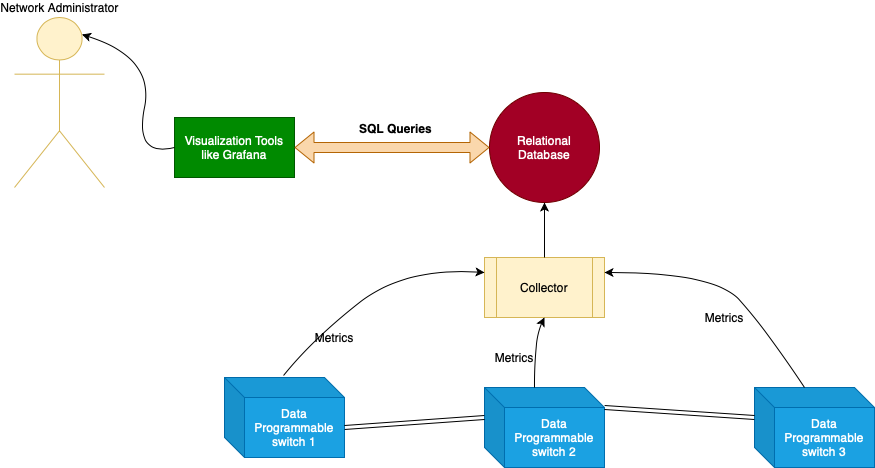
\includegraphics[width=1.0\columnwidth]{Figures/ArchitectureDiagram.png}
		\rule{35em}{0.5pt}
	\caption[Architecture Diagram]{Architecture Diagram of proposed system}
	\label{fig:Architecture Diagram}
\end{figure}
% Chapter 1

\chapter{Background Literature} % Main chapter title

\label{Chapter2} % For referencing the chapter elsewhere, use \ref{Chapter1} 

\lhead{Chapter 2. \emph{Background Knowledge}} % This is for the header on each page - perhaps a shortened title

%----------------------------------------------------------------------------------------

Historically, computer networks have always been relatively blackboxed entities that provide no substantial
facilities for configuration. The devices that are present in them, from traditional switches and routers, to other
middleware like firewalls and network address translators, often execute software that is proprietary, and hence
rigid by nature.
\newline
These devices are configured by network aaadministrators using highly specialised interfaces that vary from vendor to 
vendor. The software for communicating with these interfaces is not centralized, and network devices need to be
individually configured to achieve the desired functionality. This frozen structure has hindered flexibility and
increased costs of managing the network effectively.
\newline
It is interesting to note that this structure was not by accident. The nascent stage Internet needed to be absolutely
reliable and fault tolerant if widespread adoption was to take place. One way to minimize failures in the network was
to make the network devices rigid and inflexible. However, the widespread adoption of the
Internet has made the question of programmable networks much more pragmatic to discuss.

\section{Why do we need programmable networks?}
The ability to remotely configure behavior of switches/routers is invaluable for a number of applications,
some of them being:
\begin{itemize}
  \item Dynamic Routing of heavy hitters
  \item Testing of new protocols/routing policies
  \item In-Network Computing
  \item Layer 4 Load Balancing
  \item Network Monitoring and Debugging (The focus of this thesis)
\end{itemize}
A programmable network is much easier to monitor and control, and network devices whose forwarding policies can be
customized can be made to behave like a router, a switch, a firewall, a NAT, or any other device we can conceptualize
within the constraints of switch programmability. This saves money and physical labour that would've been
spent in the purchase and set up of highly specific network devices. A programmable network is, by nature, facilitative
to network innovation and reduces the barrier to introduction of new protocols/policies.

\section{The idea of separation of Control Plane and Data Plane}
Software Defined Networking is an umbrella term used to address efforts made to make networks programmable. Behaviour of
traditional switches is defined in hardware, whereas 'software-defined' switches would have the programmability addressed
earlier. One important concept of SDN is \textit{the decoupling of Control and Data-plans}
Control plane usually refers to protocols like OSPF, BGP, Multicast which govern traffic handling on a higher scale. The 
data plane performs packet switching based on the policies that the control plane dictates. In a general sense, the control
plane is the intelligence layer, and the data plane is the manifestation of it in a standalone switch.
\newline
A traditional switch has the forwarding logic baked into the circuit, and has tight integration of data and control planes.
The idea behind SDN is to decouple the planes, and have a programmable control plane that can communicate with the data plane
via a standardized API (like OpenFlow) so as to offer freedom in specifying how a switch handles packets.

\section{A Brief History of Programmability in Computer Networks}
\subsection{Early approaches towards programmability (1990s - late 2000s)}
The early days of SDN are majorly about the concept of Active Networks. In this, two approaches were used:
\begin{itemize}
  \item \textit{Capsule model}, where code to be run at the nodes is carried within packets
  \item \textit{Programmable router/switch model} where the code is pushed to the nodes by out-of-band means 
\end{itemize}

While capsule models were feasible, there were concerns about attackers injecting malicious code into a router and compromising
the network. The programmable model was much more aligned to what SDN is today. Most of the criticism towards these approaches 
was due to a mixture of concerns over reliability and performance, and also because it was important to ensure proliferation
of the Internet by keeping the network core as simple as possible.
\subsection{OpenFlow (and its limitations)}
OpenFlow started off as a research project implemented at Stanford University by researchers in a controlled environment. As 
mentioned before, it defines the API for communication between a decoupled data plane and control plane. OpenFlow quickly became
popular due to it being easy to adopt (most commodity switches required a firmware upgrade). The OpenFlow specification provides 
means to specify entries in match-action tables(called rules) where a match is made against the headers of the packet, and an
action is taken(forwarding, dropping, broadcasting). Widespread adoption by companies like Google gave a boost to its popularity
and many new vendors came into the established markets by early support of OpenFlow.
\newline
There is a false belief that OpenFlow is the same as SDN; SDN is a general term used for making networks programmable, whereas
OpenFlow is one concrete way to do it.
\newline
OpenFlow however, does not offer any data plane programmability support. There is no means to specify new protocols and fields to 
match against, or on how to perform reassembly of packets; consider a scenario where one needs to test a new protocol. OpenFlow
enabled switches will not be able to perform match-actions on fields specified in the protocol and will have to wait until that
protocol gets added into the specification (which can take of the order of months/years). This use case motivates the desire to make the
data plane itself programmable.
\section{Towards Data Plane Programmability}
Data plane programming offers the flexibility of describing how the packet headers can be parsed and matched onto non-standard
fields and modified (for example, those of a new protocol), as well as the order in which the headers are reassembled before being
transmitted by the switch. Programmable switches have been made possible by recent networking architectures and expose such functionality
in the data plane:
\begin{itemize}
  \item Flexible parsing
  \item Ingress/Egress processing using match-action tables
  \item Stateful maintenance of network states using SRAMs
\end{itemize}
These switches offer throughputs of close to 1 Tbps (the rate demanded by modern data centres) even with the ability to process and modify the packet. Such speeds would be impossible if packet processing was to happen in CPU due to various overheads, which is what makes data plane programmability so attractive.
\newline
\rule{\textwidth}{0.4pt}
\begin{figure}[htbp]
	\centering
		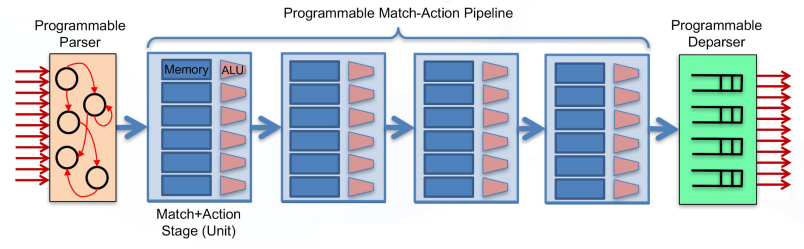
\includegraphics[width=1.0\columnwidth]{Figures/MatchAction.png}
		\rule{35em}{0.5pt}
	\caption[Match Action Pipeline]{Generic Data Programmable Switch Architecture}
	\label{fig:Match Action}
\end{figure}

\subsection{Constraints in data plane programmable switches}
In order to maintain processing at line-rate with no slow down, certain constraints need to be followed which impose a limit on the packet processing flexibility. Some of these are:
\begin{itemize}
  \item No looping constructs in P4 (language used to program switches)
  \item no floating point computations
  \item no exact multiply/divides (only approximated by bit-shifts)
  \item only one read-modify-write per stage to maintain processing at line rate
\end{itemize}
Even so, data plane programmability has found a number of applications in recent years including Network Monitoring and Debugging (the subject matter of this thesis), time synchronization, detection of elephant or heavy hitter flows, and In-network Computing.
\subsection{The P4 Programming Language}

P4 (\textit{Programming Protocol Independent Packet Processors}) is a programming language developed specifically for programming data plane switches. The language is maintained by the P4 Language Consortium and is widely used for data plane programmability today. It provides constructs for specifying deterministic parsers for header parsing, action constructs for specifying steps to be taken in case of a match, and also steps to be taken in packet reassembly.
%----------------------------------------------------------------------------------------

% \section{Getting Started with this Template}

% If you are familiar with \LaTeX{}, then you can familiarise yourself with the contents of the Zip file and the directory structure and then place your own information into the `\texttt{Thesis.cls}' file. Section \ref{FillingFile} on page \pageref{FillingFile} tells you how to do this. Make sure you read section \ref{ThesisConventions} about thesis conventions to get the most out of this template and then get started with the `\texttt{Thesis.tex}' file straightaway.

% If you are new to \LaTeX{} it is recommended that you carry on reading through the rest of the information in this document.

% \subsection{About this Template}

% This \LaTeX{} Thesis Template is originally based and created around a \LaTeX{} style file created by Steve R.\ Gunn from the University of Southampton (UK), department of Electronics and Computer Science. You can find his original thesis style file at his site, here:\\
% \href{http://www.ecs.soton.ac.uk/~srg/softwaretools/document/templates/}{\texttt{http://www.ecs.soton.ac.uk/$\sim$srg/softwaretools/document/templates/}}

% My thesis originally used the `\texttt{ecsthesis.cls}' from his list of styles. However, I knew \LaTeX{} could still format better. To get the look I wanted, I modified his style and also created a skeleton framework and folder structure to place the thesis files in.

% This Thesis Template consists of that modified style, the framework and the folder structure. All the work that has gone into the preparation and groundwork means that all you have to bother about is the writing.

% Before you begin using this template you should ensure that its style complies with the thesis style guidelines imposed by your institution. In most cases this template style and layout will be suitable. If it is not, it may only require a small change to bring the template in line with your institution's recommendations.

% %----------------------------------------------------------------------------------------

% \section{What this Template Includes}

% \subsection{Folders}

% This template comes as a single Zip file that expands out to many files and folders. The folder names are mostly self-explanatory:

% \textbf{Appendices} -- this is the folder where you put the appendices. Each appendix should go into its own separate `\texttt{.tex}' file. A template is included in the directory.

% \textbf{Chapters} -- this is the folder where you put the thesis chapters. A thesis usually has about seven chapters, though there is no hard rule on this. Each chapter should go in its own separate `\texttt{.tex}' file and they usually are split as:
% \begin{itemize}
% \item Chapter 1: Introduction to the thesis topic
% \item Chapter 2: Background information and theory
% \item Chapter 3: (Laboratory) experimental setup
% \item Chapter 4: Details of experiment 1
% \item Chapter 5: Details of experiment 2
% \item Chapter 6: Discussion of the experimental results
% \item Chapter 7: Conclusion and future directions
% \end{itemize}
% This chapter layout is specialised for the experimental sciences.

% \textbf{Figures} -- this folder contains all figures for the thesis. These are the final images that will go into the thesis document.

% \textbf{Primitives} -- this is the folder that contains scraps, particularly because one final image in the `Figures' folder may be made from many separate images and photos, these source images go here. This keeps the intermediate files separate from the final thesis figures.

% \subsection{Files}

% Included are also several files, most of them are plain text and you can see their contents in a text editor. Luckily, many of them are auxiliary files created by \LaTeX{} or BibTeX and which you don't need to bother about:

% \textbf{Bibliography.bib} -- this is an important file that contains all the bibliographic information and references that you will be citing in the thesis for use with BibTeX. You can write it manually, but there are reference manager programs available that will create and manage it for you. Bibliographies in \LaTeX{} are a large subject and you may need to read about BibTeX before starting with this.

% \textbf{Thesis.cls} -- this is an important file. It is the style file that tells \LaTeX{} how to format the thesis. You will also need to open this file in a text editor and fill in your own information (such as name, department, institution). Luckily, this is not too difficult and is explained in section \ref{FillingFile} on page \pageref{FillingFile}.

% \textbf{Thesis.pdf} -- this is your beautifully typeset thesis (in the PDF file format) created by \LaTeX{}.

% \textbf{Thesis.tex} -- this is an important file. This is the file that you tell \LaTeX{} to compile to produce your thesis as a PDF file. It contains the framework and constructs that tell \LaTeX{} how to layout the thesis. It is heavily commented so you can read exactly what each line of code does and why it is there. After you put your own information into the `\texttt{Thesis.cls}' file, go to this file and begin filling it in -- you have now started your thesis!

% \textbf{vector.sty} -- this is a \LaTeX{} package, it tells \LaTeX{} how to typeset mathematical vectors. Using this package is very easy and you can read the documentation on the site (you just need to look at the `\texttt{vector.pdf}' file):\\
% \href{http://www.ctan.org/tex-archive/macros/latex/contrib/vector/}{\texttt{http://www.ctan.org/tex-archive/macros/latex/contrib/vector/}}

% \textbf{lstpatch.sty} -- this is a \LaTeX{} package required by this LaTeX template and is included as not all \TeX{} distributions have it installed by default. You do not need to modify this file.

% Files that are \emph{not} included, but are created by \LaTeX{} as auxiliary files include:

% \textbf{Thesis.aux} -- this is an auxiliary file generated by \LaTeX{}, if it is deleted \LaTeX{} simply regenerates it when you run the main `\texttt{.tex}' file.

% \textbf{Thesis.bbl} -- this is an auxiliary file generated by BibTeX, if it is deleted, BibTeX simply regenerates it when you run the main tex file. Whereas the `\texttt{.bib}' file contains all the references you have, this `\texttt{.bbl}' file contains the references you have actually cited in the thesis and is used to build the bibliography section of the thesis.

% \textbf{Thesis.blg} -- this is an auxiliary file generated by BibTeX, if it is deleted BibTeX simply regenerates it when you run the main `\texttt{.tex}' file.

% \textbf{Thesis.lof} -- this is an auxiliary file generated by \LaTeX{}, if it is deleted \LaTeX{} simply regenerates it when you run the main `\texttt{.tex}' file. It tells \LaTeX{} how to build the `List of Figures' section.

% \textbf{Thesis.log} -- this is an auxiliary file generated by \LaTeX{}, if it is deleted \LaTeX{} simply regenerates it when you run the main `\texttt{.tex}' file. It contains messages from \LaTeX{}, if you receive errors and warnings from \LaTeX{}, they will be in this `\texttt{.log}' file.

% \textbf{Thesis.lot} -- this is an auxiliary file generated by \LaTeX{}, if it is deleted \LaTeX{} simply regenerates it when you run the main `\texttt{.tex}' file. It tells \LaTeX{} how to build the `List of Tables' section.

% \textbf{Thesis.out} -- this is an auxiliary file generated by \LaTeX{}, if it is deleted \LaTeX{} simply regenerates it when you run the main `\texttt{.tex}' file.


% So from this long list, only the files with the `\texttt{.sty}', `\texttt{.bib}', `\texttt{.cls}' and `\texttt{.tex}' extensions are the most important ones. The other auxiliary files can be ignored or deleted as \LaTeX{} and BibTeX will regenerate them.

% %----------------------------------------------------------------------------------------

% \section{Filling in the `\texttt{Thesis.cls}' File}\label{FillingFile}

% You will need to personalise the thesis template and make it your own by filling in your own information. This is done by editing the `\texttt{Thesis.cls}' file in a text editor.

% Open the file and scroll down, past all the `$\backslash$\texttt{newcommand}\ldots' items until you see the entries for `\texttt{University Name}', `\texttt{Department Name}', etc\ldots.

% Fill out the information about your group and institution and ensure you keep to block capitals where it asks you to. You can also insert web links, if you do, make sure you use the full URL, including the `\texttt{http://}' for this.

% The last item you should need to fill in is the Faculty Name (in block capitals). When you have done this, save the file and recompile `\texttt{Thesis.tex}'. All the information you filled in should now be in the PDF, complete with web links. You can now begin your thesis proper!

% %----------------------------------------------------------------------------------------

% \section{The `\texttt{Thesis.tex}' File Explained}

% The \texttt{Thesis.tex} file contains the structure of the thesis. There are plenty of written comments that explain what pages, sections and formatting the \LaTeX{} code is creating. Initially there seems to be a lot of \LaTeX{} code, but this is all formatting, and it has all been taken care of so you don't have to do it.

% Begin by checking that your information on the title page is correct. For the thesis declaration, your institution may insist on something different than the text given. If this is the case, just replace what you see with what is required.

% Then comes a page which contains a funny quote. You can put your own, or quote your favourite scientist, author, person, etc\ldots Make sure to put the name of the person who you took the quote from.

% Next comes the acknowledgements. On this page, write about all the people who you wish to thank (not forgetting parents, partners and your advisor/supervisor).

% The contents pages, list of figures and tables are all taken care of for you and do not need to be manually created or edited. The next set of pages are optional and can be deleted since they are for a more technical thesis: insert a list of abbreviations you have used in the thesis, then a list of the physical constants and numbers you refer to and finally, a list of mathematical symbols used in any formulae. Making the effort to fill these tables means the reader has a one-stop place to refer to instead of searching the internet and references to try and find out what you meant by certain abbreviations or symbols.

% The list of symbols is split into the Roman and Greek alphabets. Whereas the abbreviations and symbols ought to be listed in alphabetical order (and this is \emph{not} done automatically for you) the list of physical constants should be grouped into similar themes.

% The next page contains a one line dedication. Who will you dedicate your thesis to?

% Finally, there is the section where the chapters are included. Uncomment the lines (delete the `\texttt{\%}' character) as you write the chapters. Each chapter should be written in its own file and put into the `Chapters' folder and named `\texttt{Chapter1}', `\texttt{Chapter2}, etc\ldots Similarly for the appendices, uncomment the lines as you need them. Each appendix should go into its own file and placed in the `Appendices' folder.

% After the preamble, chapters and appendices finally comes the bibliography. The bibliography style (called `\texttt{unsrtnat}') is used for the bibliography and is a fully featured style that will even include links to where the referenced paper can be found online. Do not under estimate how grateful you reader will be to find that a reference to a paper is just a click away. Of course, this relies on you putting the URL information into the BibTeX file in the first place.

% %----------------------------------------------------------------------------------------

% \section{Thesis Features and Conventions}\label{ThesisConventions}

% To get the best out of this template, there are a few conventions that you may want to follow.

% One of the most important (and most difficult) things to keep track of in such a long document as a thesis is consistency. Using certain conventions and ways of doing things (such as using a Todo list) makes the job easier. Of course, all of these are optional and you can adopt your own method.

% \subsection{Printing Format}

% This thesis template is designed for single sided printing as most theses are printed and bound this way. This means that the left margin is always wider than the right (for binding). Four out of five people will now judge the margins by eye and think, ``I never 
% noticed that before.''.

% The headers for the pages contain the page number on the right side (so it is easy to flick through to the page you want) and the chapter name on the left side.

% The text is set to 11 point and a line spacing of 1.3. Generally, it is much more readable to have a smaller text size and wider gap between the lines than it is to have a larger text size and smaller gap. Again, you can tune the text size and spacing should you want or need to. The text size can be set in the options for the `$\backslash$\texttt{documentclass}' command at the top of the `\texttt{Thesis.tex}' file and the spacing can be changed by setting a different value in the `$\backslash$\texttt{setstretch}' commands (scattered throughout the `\texttt{Thesis.tex}' file).

% \subsection{Using US Letter Paper}

% The paper size used in the template is A4, which is a common -- if not standard -- size in Europe. If you are using this thesis template elsewhere and particularly in the United States, then you may have to change the A4 paper size to the US Letter size. Unfortunately, this is not as simple as replacing instances of `\texttt{a4paper}' with `\texttt{letterpaper}'.

% This is because the final PDF file is created directly from the \LaTeX{} source using a program called `\texttt{pdfTeX}' and in certain conditions, paper size commands are ignored and all documents are created with the paper size set to the size stated in the configuration file for pdfTeX (called `\texttt{pdftex.cfg}').

% What needs to be done is to change the paper size in the configuration file for \texttt{pdfTeX} to reflect the letter size. There is an excellent tutorial on how to do this here: \\
% \href{http://www.physics.wm.edu/~norman/latexhints/pdf_papersize.html}{\texttt{http://www.physics.wm.edu/$\sim$norman/latexhints/pdf\_papersize.html}}

% It may be sufficient just to replace the dimensions of the A4 paper size with the US Letter size in the \texttt{pdftex.cfg} file. Due to the differences in the paper size, the resulting margins may be different to what you like or require (as it is common for Institutions to dictate certain margin sizes). If this is the case, then the margin sizes can be tweaked by opening up the \texttt{Thesis.cls} file and searching for the line beginning with, `$\backslash$\texttt{setmarginsrb}' (not very far down from the top), there you will see the margins specified. Simply change those values to what you need (or what looks good) and save. Now your document should be set up for US Letter paper size with suitable margins.

% \subsection{References}

% The `\texttt{natbib}' package is used to format the bibliography and inserts references such as this one \cite{cmu-malware}. The options used in the `\texttt{Thesis.tex}' file mean that the references are listed in numerical order as they appear in the text. Multiple references are rearranged in numerical order (e.g. \cite{kendall2007practical}). This is done automatically for you. To see how you use references, have a look at the `\texttt{Chapter1.tex}' source file. Many reference managers allow you to simply drag the reference into the document as you type.

% Scientific references should come \emph{before} the punctuation mark if there is one (such as a comma or period). The same goes for footnotes\footnote{Such as this footnote, here down at the bottom of the page.}. You can change this but the most important thing is to keep the convention consistent throughout the thesis. Footnotes themselves should be full, descriptive sentences (beginning with a capital letter and ending with a full stop).

% To see how \LaTeX{} typesets the bibliography, have a look at the very end of this document (or just click on the reference number links).

%----------------------------------------------------------------------------------------

%% Chapter Template

\chapter{Data Centres and Data Centre Traffic} % Main chapter title

\label{Chapter3} % Change X to a consecutive number; for referencing this chapter elsewhere, use \ref{ChapterX}

\lhead{Chapter 3. \emph{Data Centres and Data Centre Traffic}} % Change X to a consecutive number; this is for the header on each page - perhaps a shortened title

%----------------------------------------------------------------------------------------
%	SECTION 1
%----------------------------------------------------------------------------------------

\section{Main Section 1}


%-----------------------------------
%	SUBSECTION 1
%-----------------------------------
\subsection{Subsection 1}


%-----------------------------------
%	SUBSECTION 2
%-----------------------------------

\subsection{Subsection 2}

%----------------------------------------------------------------------------------------
%	SECTION 2
%----------------------------------------------------------------------------------------

\section{Main Section 2}


%% Chapter Template

\chapter{Extracting insights from Relational Data} % Main chapter title

\label{Chapter4} % Change X to a consecutive number; for referencing this chapter elsewhere, use \ref{ChapterX}

\lhead{Chapter 4. \emph{Extracting insights from Relational Data}} % Change X to a consecutive number; this is for the header on each page - perhaps a shortened title

%----------------------------------------------------------------------------------------
%	SECTION 1
%----------------------------------------------------------------------------------------

\section{Description of Methodology}

The relational schema available for each collection trace and the meaning of each of the fields collected has been described in \ref{Chapter3}.
In this section, the various preprocessing done on each scenario so as to derive useful quantities for visualizing the network and understanding
what exactly is happening in the network is described. All preprocessing code \url{https://github.com/sankalp-sangle/FlaskDebugger/blob/master/preprocess.py} is written in Python3
and the mysql.connector library is used for communication with the MySQL database.
\newline
We describe how to derive three quantities from the existing schema described earlier. The usefulness of these quantities will be shown in Chapter 5.

\begin{itemize}
    \item Time Series of relative ratio of packets in queue for each flow (as defined by source IP) in each switch in the network.
    \item Ingress throughput for each flow in each switch in the network.
    \item Egress throughput for every link as seen in the network.
\end{itemize}

\section{Time Series of relative ratio of packets in queue for each flow}

\subsection{Motivation}
This quantity helps to understand the composition of the queue in a switch at any point in time. By composition, we mean that if, at a point \emph{t} in time,
the size of the queue in a switch is \emph{S} packets, and the number of packets of a flow \emph{i} is \emph{n}, then our plan is to compute \emph{n} / \emph{S} for all flows
at evenly spaced points of time. We do this for all switches. Having a plot of this quantity will help us understand how the distribution of a queue changes as packets arrive
and leave the queue.

\subsection{Computation}
We use the following process for computing the quantity described above.

\begin{enumerate}
    \item Select an interval I which will serve as the gap between successful computations of the relative ratios.
    \item For a point in time \emph{Tcurrent}, perform the following query on the Packetrecords table.
    \begin{verbatim}
    SELECT source_ip, COUNT(hash) 
    FROM packetrecords
    WHERE time_in < Tcurrent AND time_out > Tcurrent
    GROUP BY source_ip;
    \end{verbatim}
    \item This query returns to us the list of flows inside the queue of a switch at a particular time Tcurrent (as ensured by the WHERE clause) as well as the number of packets of
    each flow. The ratios can then be obtained by taking the sum of the packets and dividing each flows number of packets by the total number just computed.
    \item This query is then repeated at every I spaced interval (by incrementing Tcurrent by I each time) in the duration of the records of the switch.
\end{enumerate}

\subsection{Visual Result}
To show how a quantity like this will be helpful, refer to Fig. \ref{fig:QDSimple} where the queue depth has been plotted. The queue depth on it's own does not give us much information on what happened
in the switch, but the composition of the queue (Fig. \ref{fig:QDRatio} (using the relative ratio quantity computed above) gives us a much more revealing insight into how the queue built up over time.
We can clearly understand that the flow coloured in blue is the dominant flow in the queue and is probably a heavy hitter flow. Also refer to Fig. \ref{fig:QDAbsolute} where the absolute relative ratio
of flows has been plotted against time.

\begin{figure}[htbp]
	\centering
		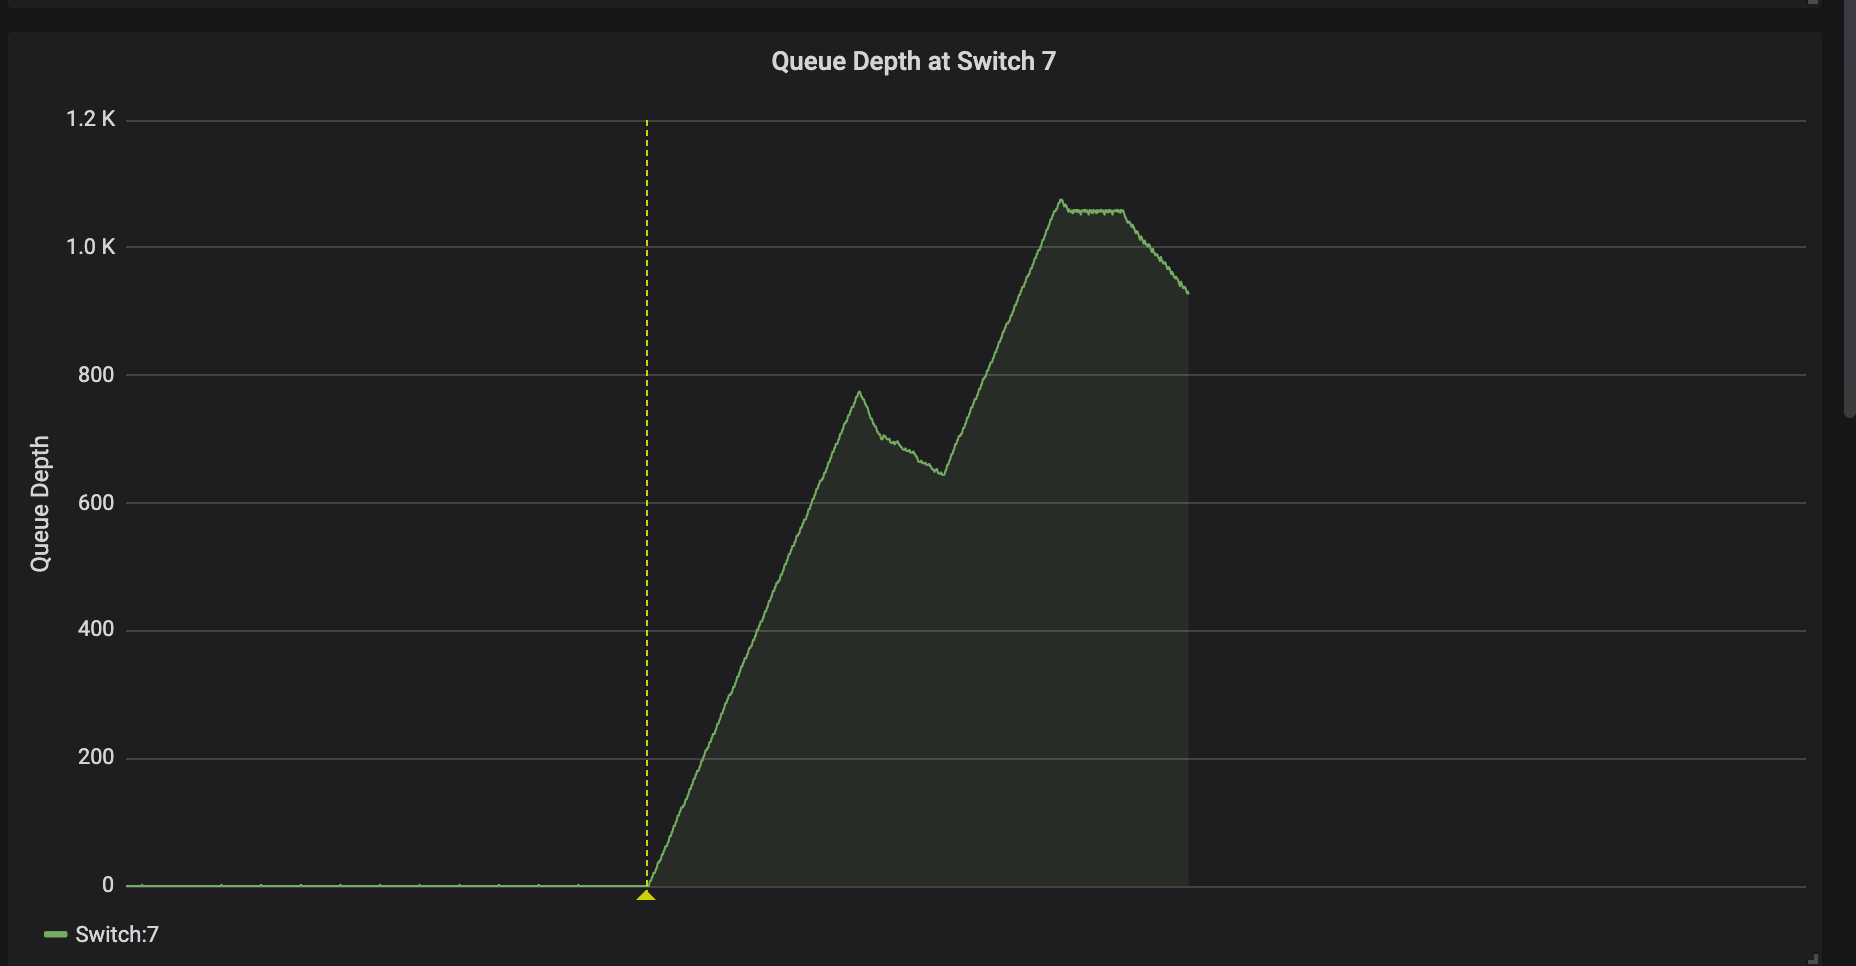
\includegraphics[width=1.0\columnwidth]{Figures/queue_depth_simple.png}
		\rule{35em}{0.5pt}
	\caption[Queue Depth Simple]{Queue Depth at a switch}
	\label{fig:QDSimple}
\end{figure}

\begin{figure}[htbp]
	\centering
		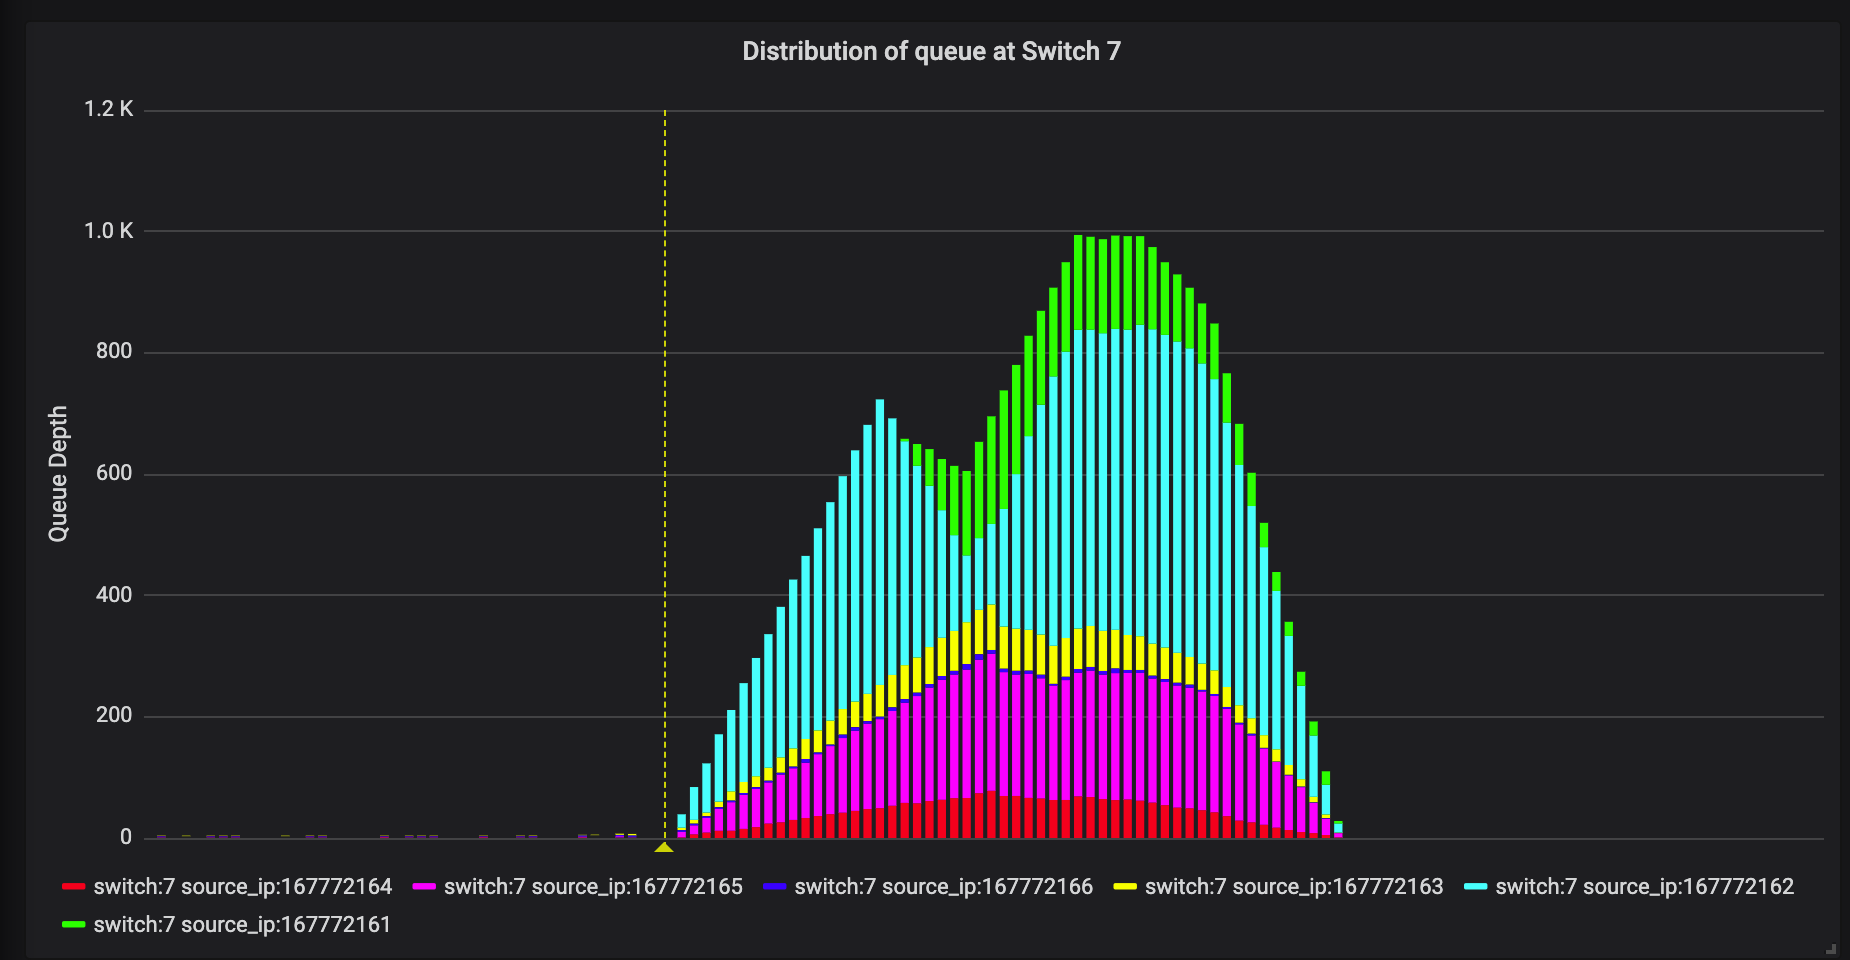
\includegraphics[width=1.0\columnwidth]{Figures/queue_depth_composition.png}
		\rule{35em}{0.5pt}
	\caption[Queue Depth composition]{Queue Depth composition at a switch. Each colour represents packets from one particular flow / source IP}
	\label{fig:QDRatio}
\end{figure}

\begin{figure}[htbp]
	\centering
		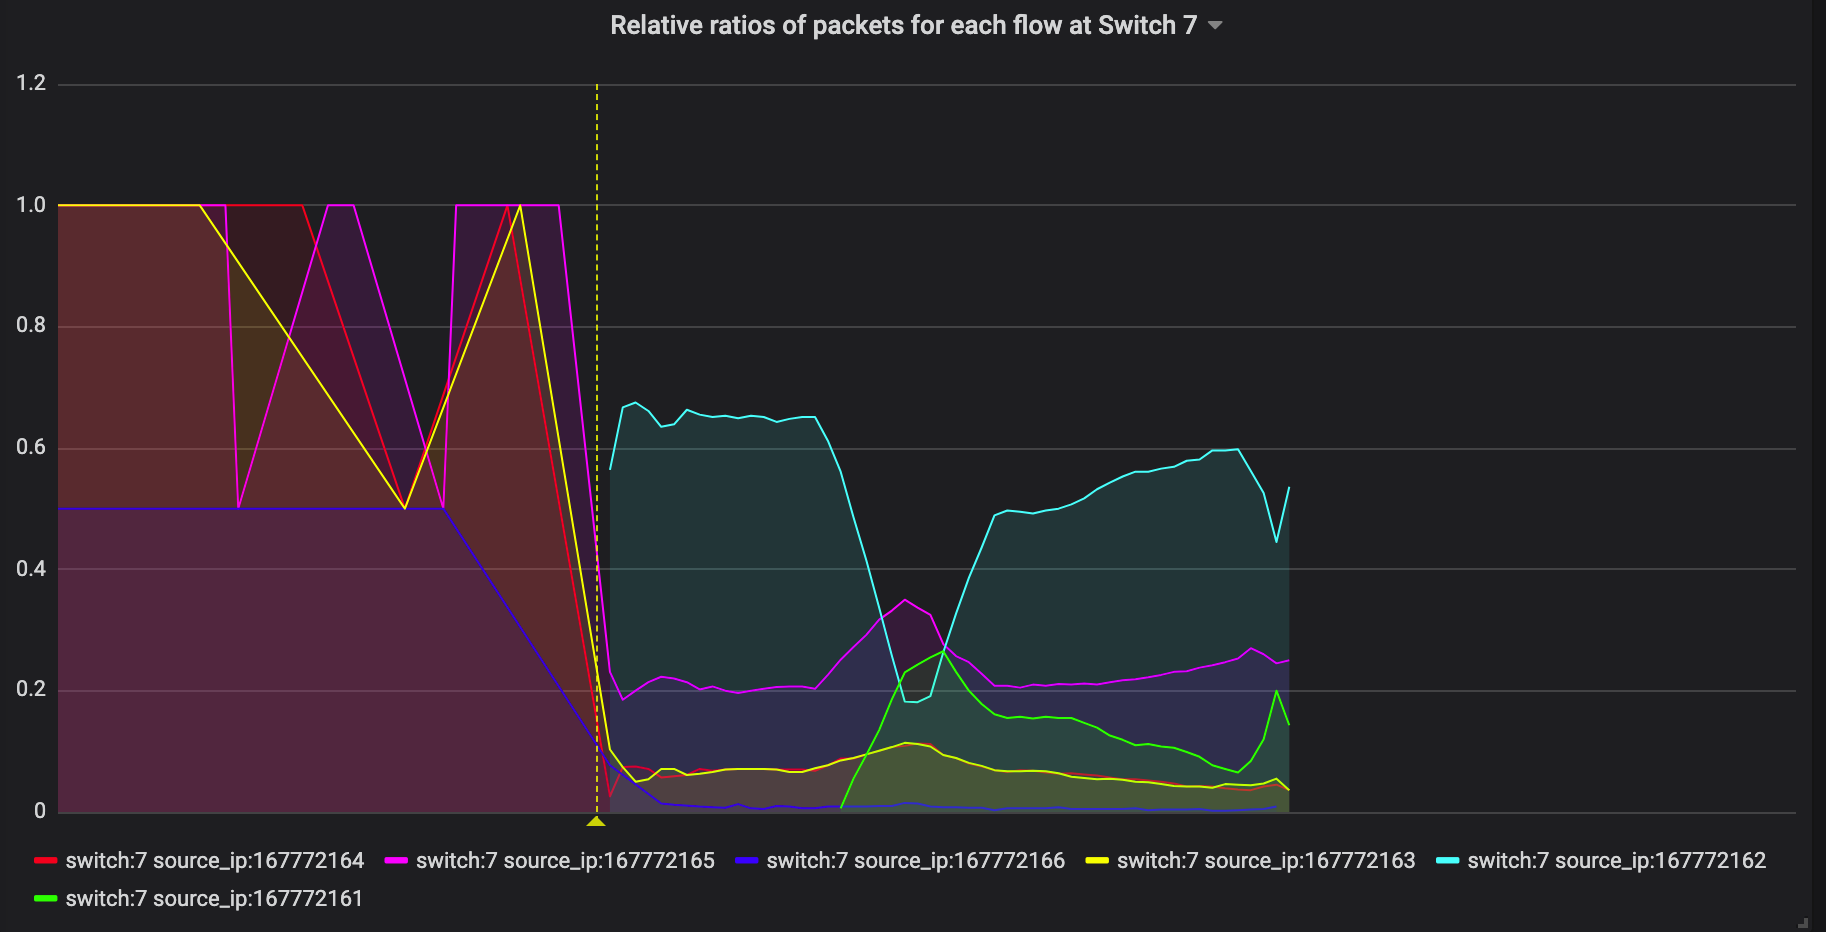
\includegraphics[width=1.0\columnwidth]{Figures/ratio_absolute.png}
		\rule{35em}{0.5pt}
	\caption[Relative Ratios]{Relative ratios for flows at a switch}
	\label{fig:QDAbsolute}
\end{figure}

\section{Ingress Throughputs for each flow in switch}

\subsection{Motivation}
This quantity captures the bandwidth of incoming flows in a switch at any point in time. This is the classical definition of bandwidth such that if, in an interval of time \emph{T},
\emph{p} number of packets of a flow enter the switch, then our plan is to compute \emph{packet size} * \emph{n} / \emph{T} for all flows
across all such intervals for a switch. We do this for all switches. Having a plot of this quantity will help us understand the distribution of incoming flows into a switch.

\subsection{Computation}
We use the following process for computing the quantity described above.

\begin{enumerate}
    \item Select an interval I which will serve as the window size for computing the throughput for a flow.
    \item For an interval \emph{ [Tleft - Tright]} in time, perform the following query on the Packetrecords table.
    \begin{verbatim}
    SELECT source_ip, COUNT(hash) 
    FROM packetrecords
    WHERE time_in > Tleft AND time_out > Tright
    GROUP BY source_ip;
    \end{verbatim}
    \item This query returns to us the list of flows that entered a switch in a particular time interval (as ensured by the WHERE clause) as well as the number of packets of
    each flow. The throughput for each flow can then be obtained by dividing the incoming number of bits (number of packets * packetsize) by the interval I (which is equal to the difference
    between Tleft and Tright).
    \item This query is then repeated at all I length intervals (by incrementing Tleft and Tright both by I each time) in the duration of the records of the switch.
\end{enumerate}

\subsection{Visual Result}
To show how a quantity like this will be helpful, refer to Fig. \ref{fig:Ing_Ind} and \ref{fig:Ing_Stacked} which represent the individual ingress throughputs as well as the stacked (sum of all) ingress throughput
for the switch. It can be seen that the ingress throughput is much more than 10 Gbps which is the capacity of the outgoing link, which is why the queue starts building up due to more packets
coming in than those being sent out for a particular interval.

\begin{figure}[htbp]
	\centering
		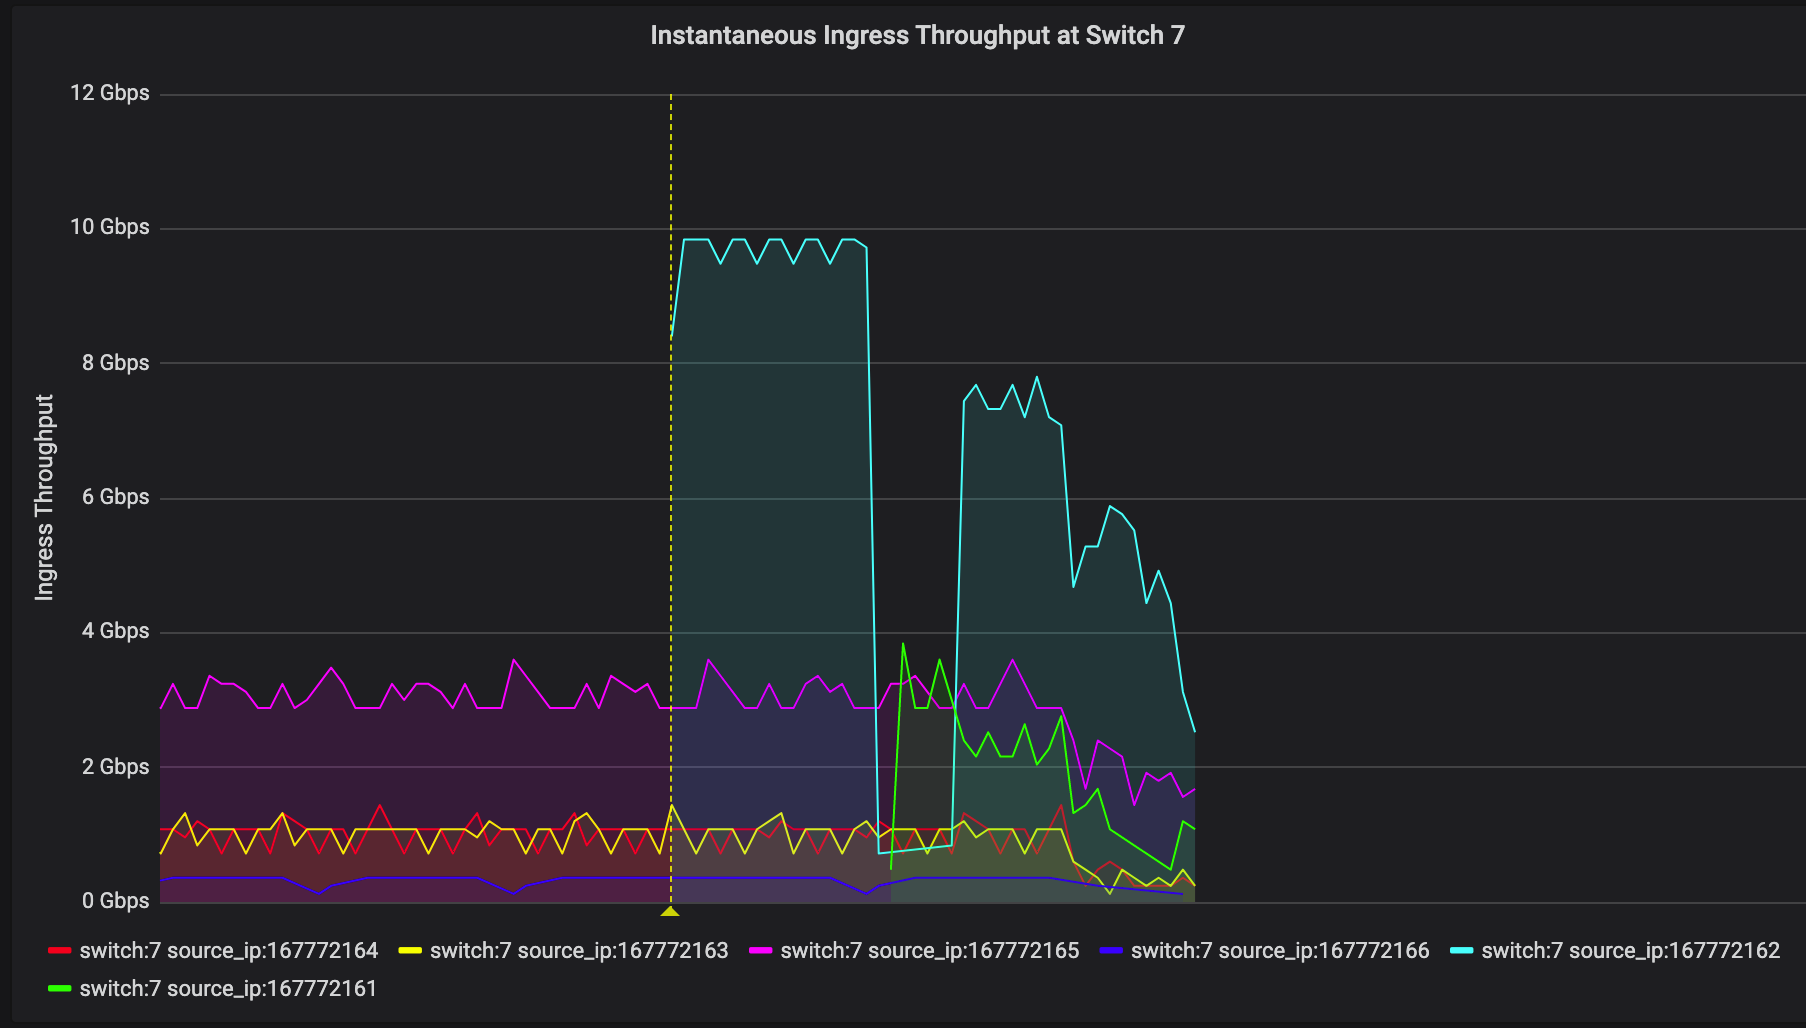
\includegraphics[width=1.0\columnwidth]{Figures/ingress_individual.png}
		\rule{35em}{0.5pt}
	\caption[Individual Ingress Throughputs]{Individual Ingress throughputs at switch}
	\label{fig:Ing_Ind}
\end{figure}

\begin{figure}[htbp]
	\centering
		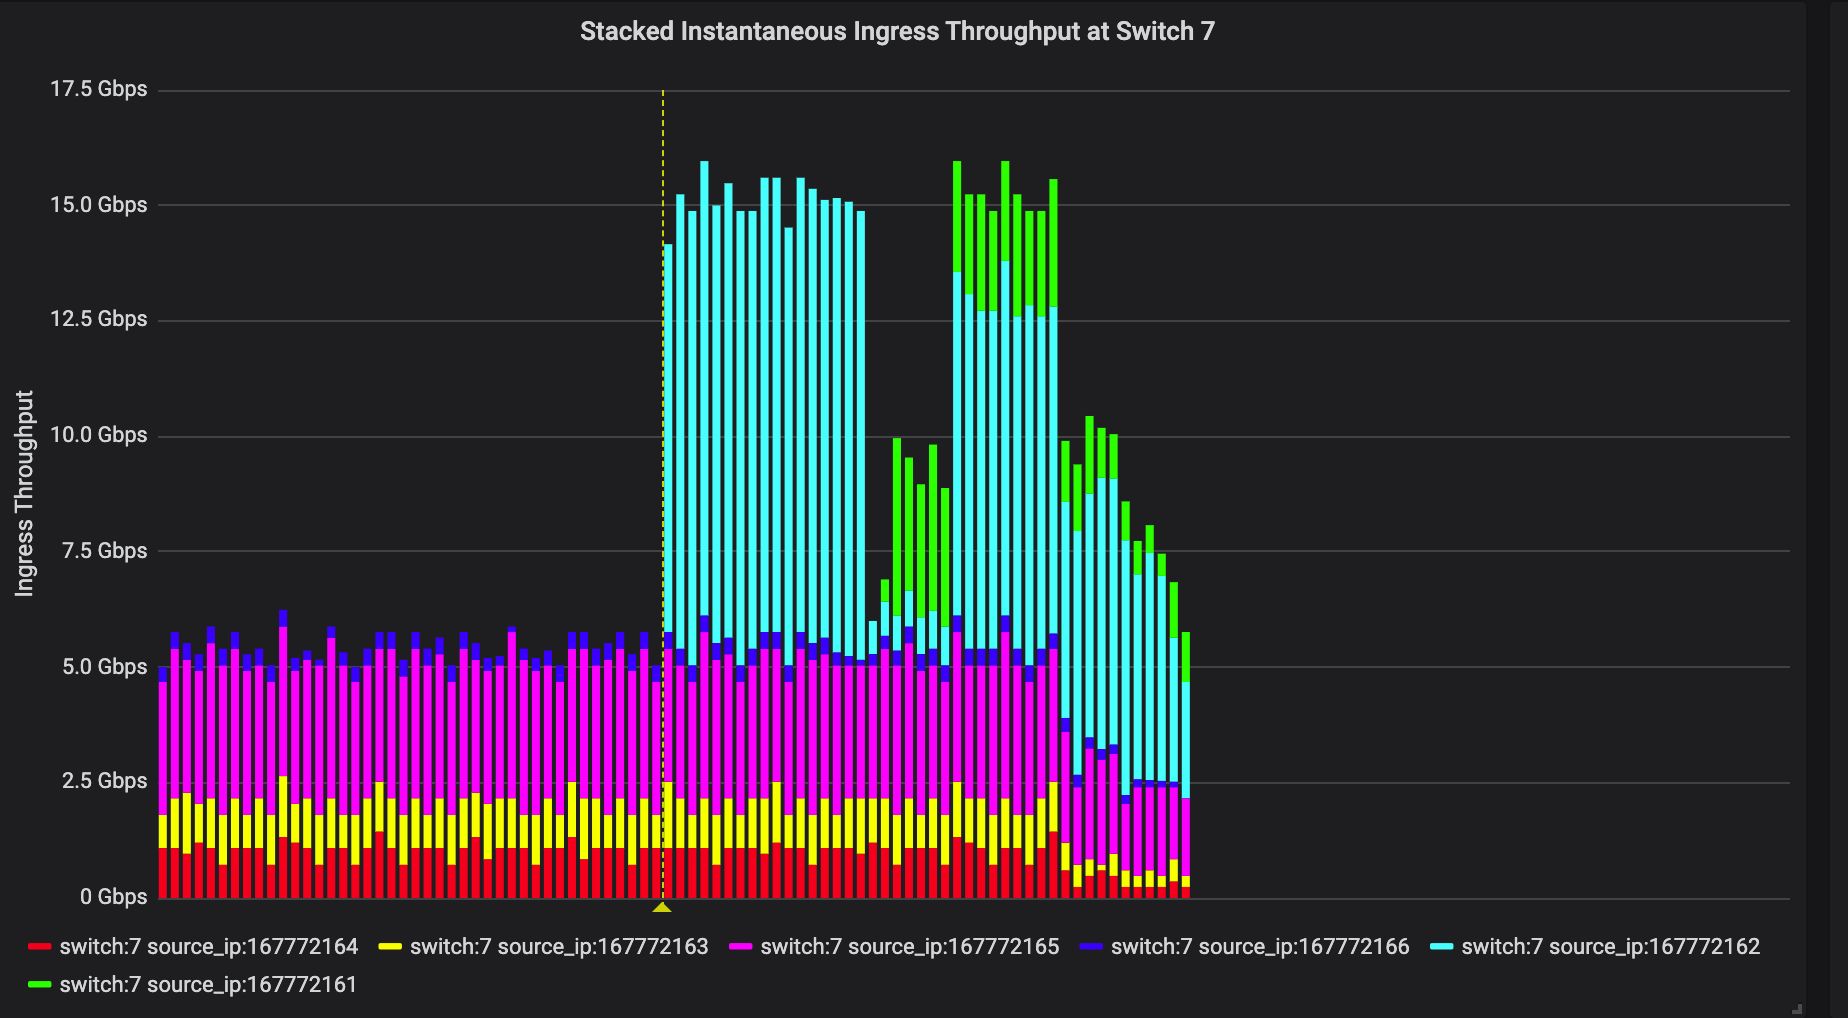
\includegraphics[width=1.0\columnwidth]{Figures/ingress_stacked.png}
		\rule{35em}{0.5pt}
	\caption[Stacked Ingress Throughputs]{Stacked Ingress throughputs at switch}
	\label{fig:Ing_Stacked}
\end{figure}

\section{Egress Throughputs for each link in network}

\subsection{Motivation}
This quantity captures the bandwidth at an interval of time for a link in the network. This is the most important quantity for creating a visualization that indicates
the bandwidth of all links at a particular point in time (Refer to Fig. \ref{})

\subsection{Computation}
The computation of bandwidth for all links in the network from the schema provided to us is a 2 step process. We firstly compute a table \emph{linkmaps} as described
below.

\begin{enumerate}
    \item Run the following query on MySQL via Python3
    \begin{verbatim}
    SELECT time_in, time_out, switch, hash
    FROM packetrecords
    ORDER BY hash, time_in;
    \end{verbatim}
    \item This query returns for us the records of a packet as it travels the network in a chronological manner. Thus if a packet visites switches S2, S3, S5, then we will
    obtain the records for that packet as captured by the switches in the order of the switch visited.
    \item From this data, we construct the table linkmaps containing the fields time enter (the timeout value of record at index i), time exit (the time in value of record at index i+1), from switch
    (the switch value of record at index i), to switch (the switch value of record at index i+1) and hash of the packet in question.
    \item Once we have constructed this linkmaps table, the process of calculating throughputs is relatively straightforward. We decide an interval I that will be the width for
    one calculation of throughput.
    \item We run the following query for a particular interval \emph{[Tleft - Tright]} for a particular switch S which we are considering as the source for links whose throughput we are calculating:
    \begin{verbatim}
    SELECT to_switch, time_exit 
    FROM linkmaps
    WHERE time_exit > Tleft AND time_exit < Tright AND from_switch = S
    GROUP BY to_switch;
    \end{verbatim}
    \item Now we collect all records going to a particular to switch, and calculate the throughput for that interval by dividing number of records times the packet size by the interval duration.
    This will be the throughput at a time (time exit) for the link represented by source as from switch and destination as to switch.
    \item This query is then repeated at all I length intervals (by incrementing Tleft and Tright both by I each time) in the duration of the records of linkmaps table.
\end{enumerate}

\subsection{Visual Result}
To show how a quantity like this will be helpful, refer to Fig. \ref{fig:Eg_Ind} the individual egress throughput on link connecting switch 9 and switch 7. It can be seen that the individual
egress throughput is constant at 10 Gbps which is the capacity of the outgoing link, showing that the link is being completely utilized.

This quantity is also extremely useful for creating visualizations like that in Fig. \ref{fig:Eg_example} which give a birds eye view of what exactly is happening in the network. This view
which can be changed over time, is invaluable for understanding what exactly happened in the network.

\begin{figure}[htbp]
	\centering
		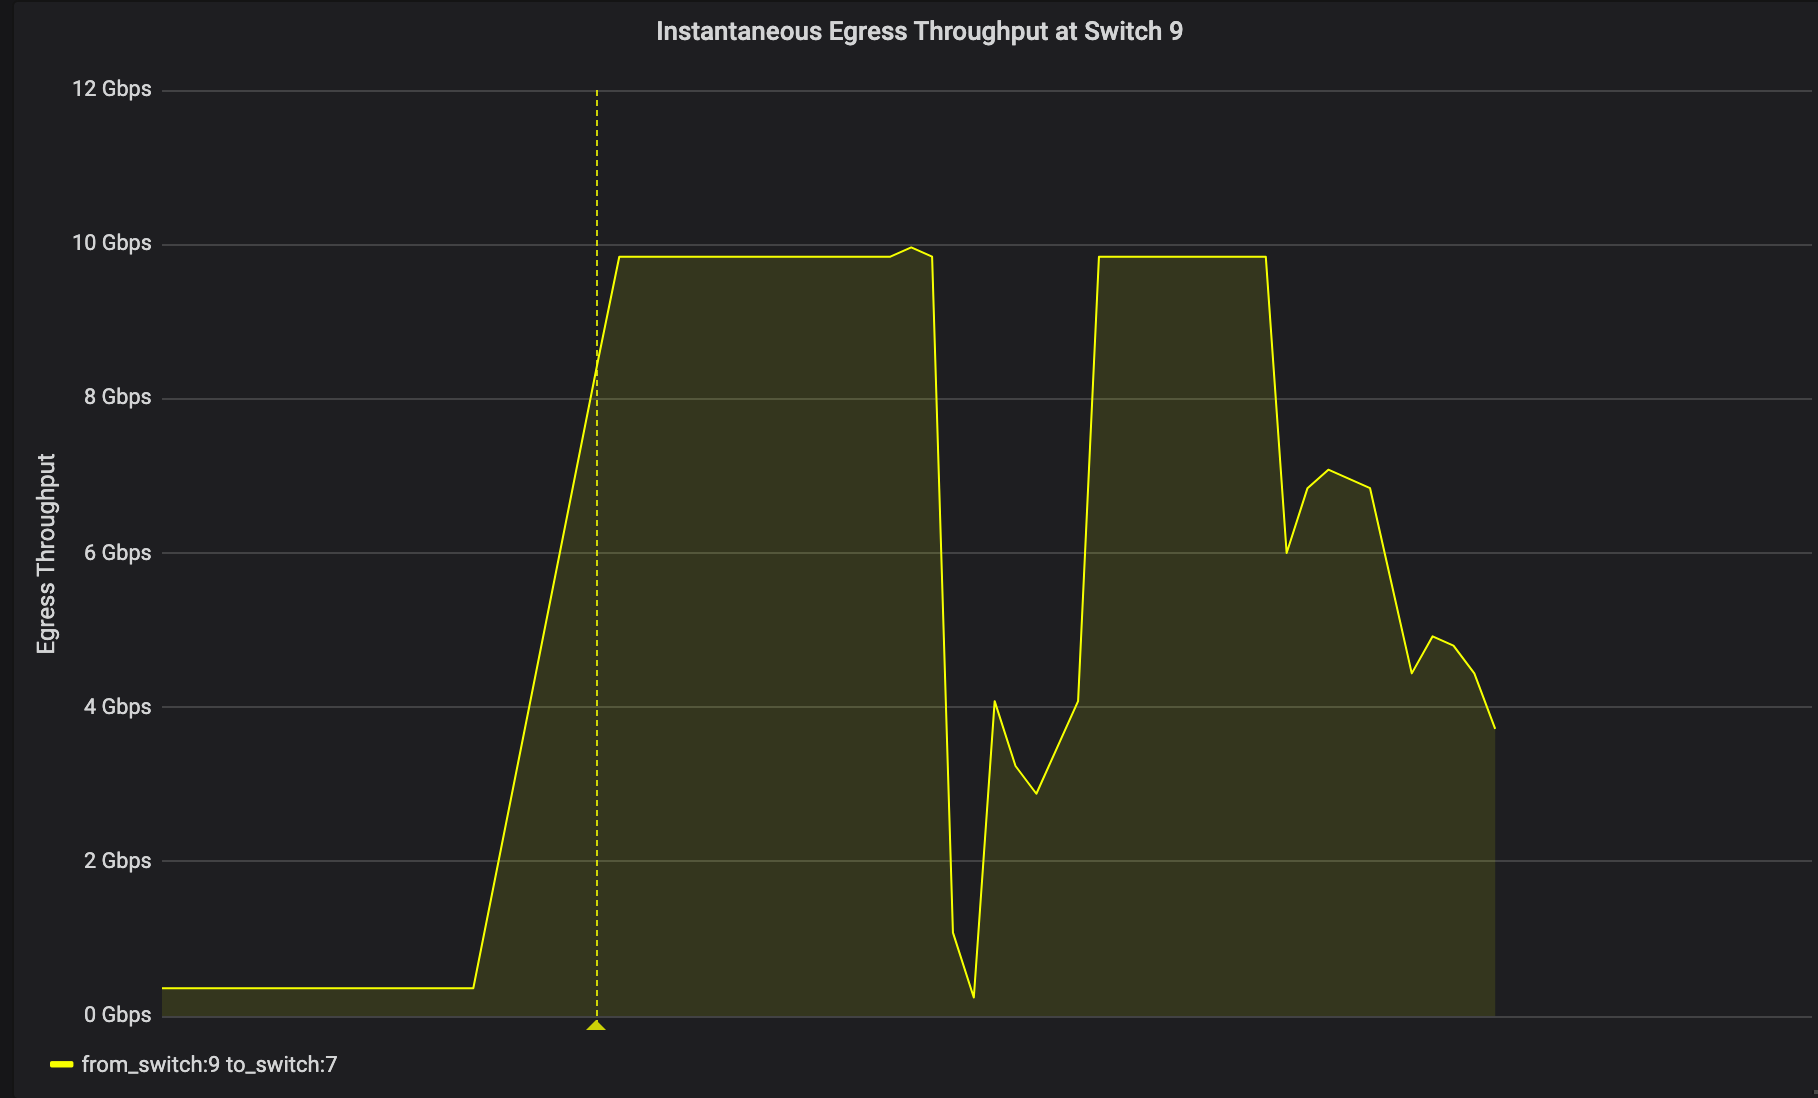
\includegraphics[width=1.0\columnwidth]{Figures/egress_individual.png}
		\rule{35em}{0.5pt}
	\caption[Individual Egress Throughputs]{Individual Engress throughput at switch}
	\label{fig:Eg_Ind}
\end{figure}

\begin{figure}[htbp]
	\centering
		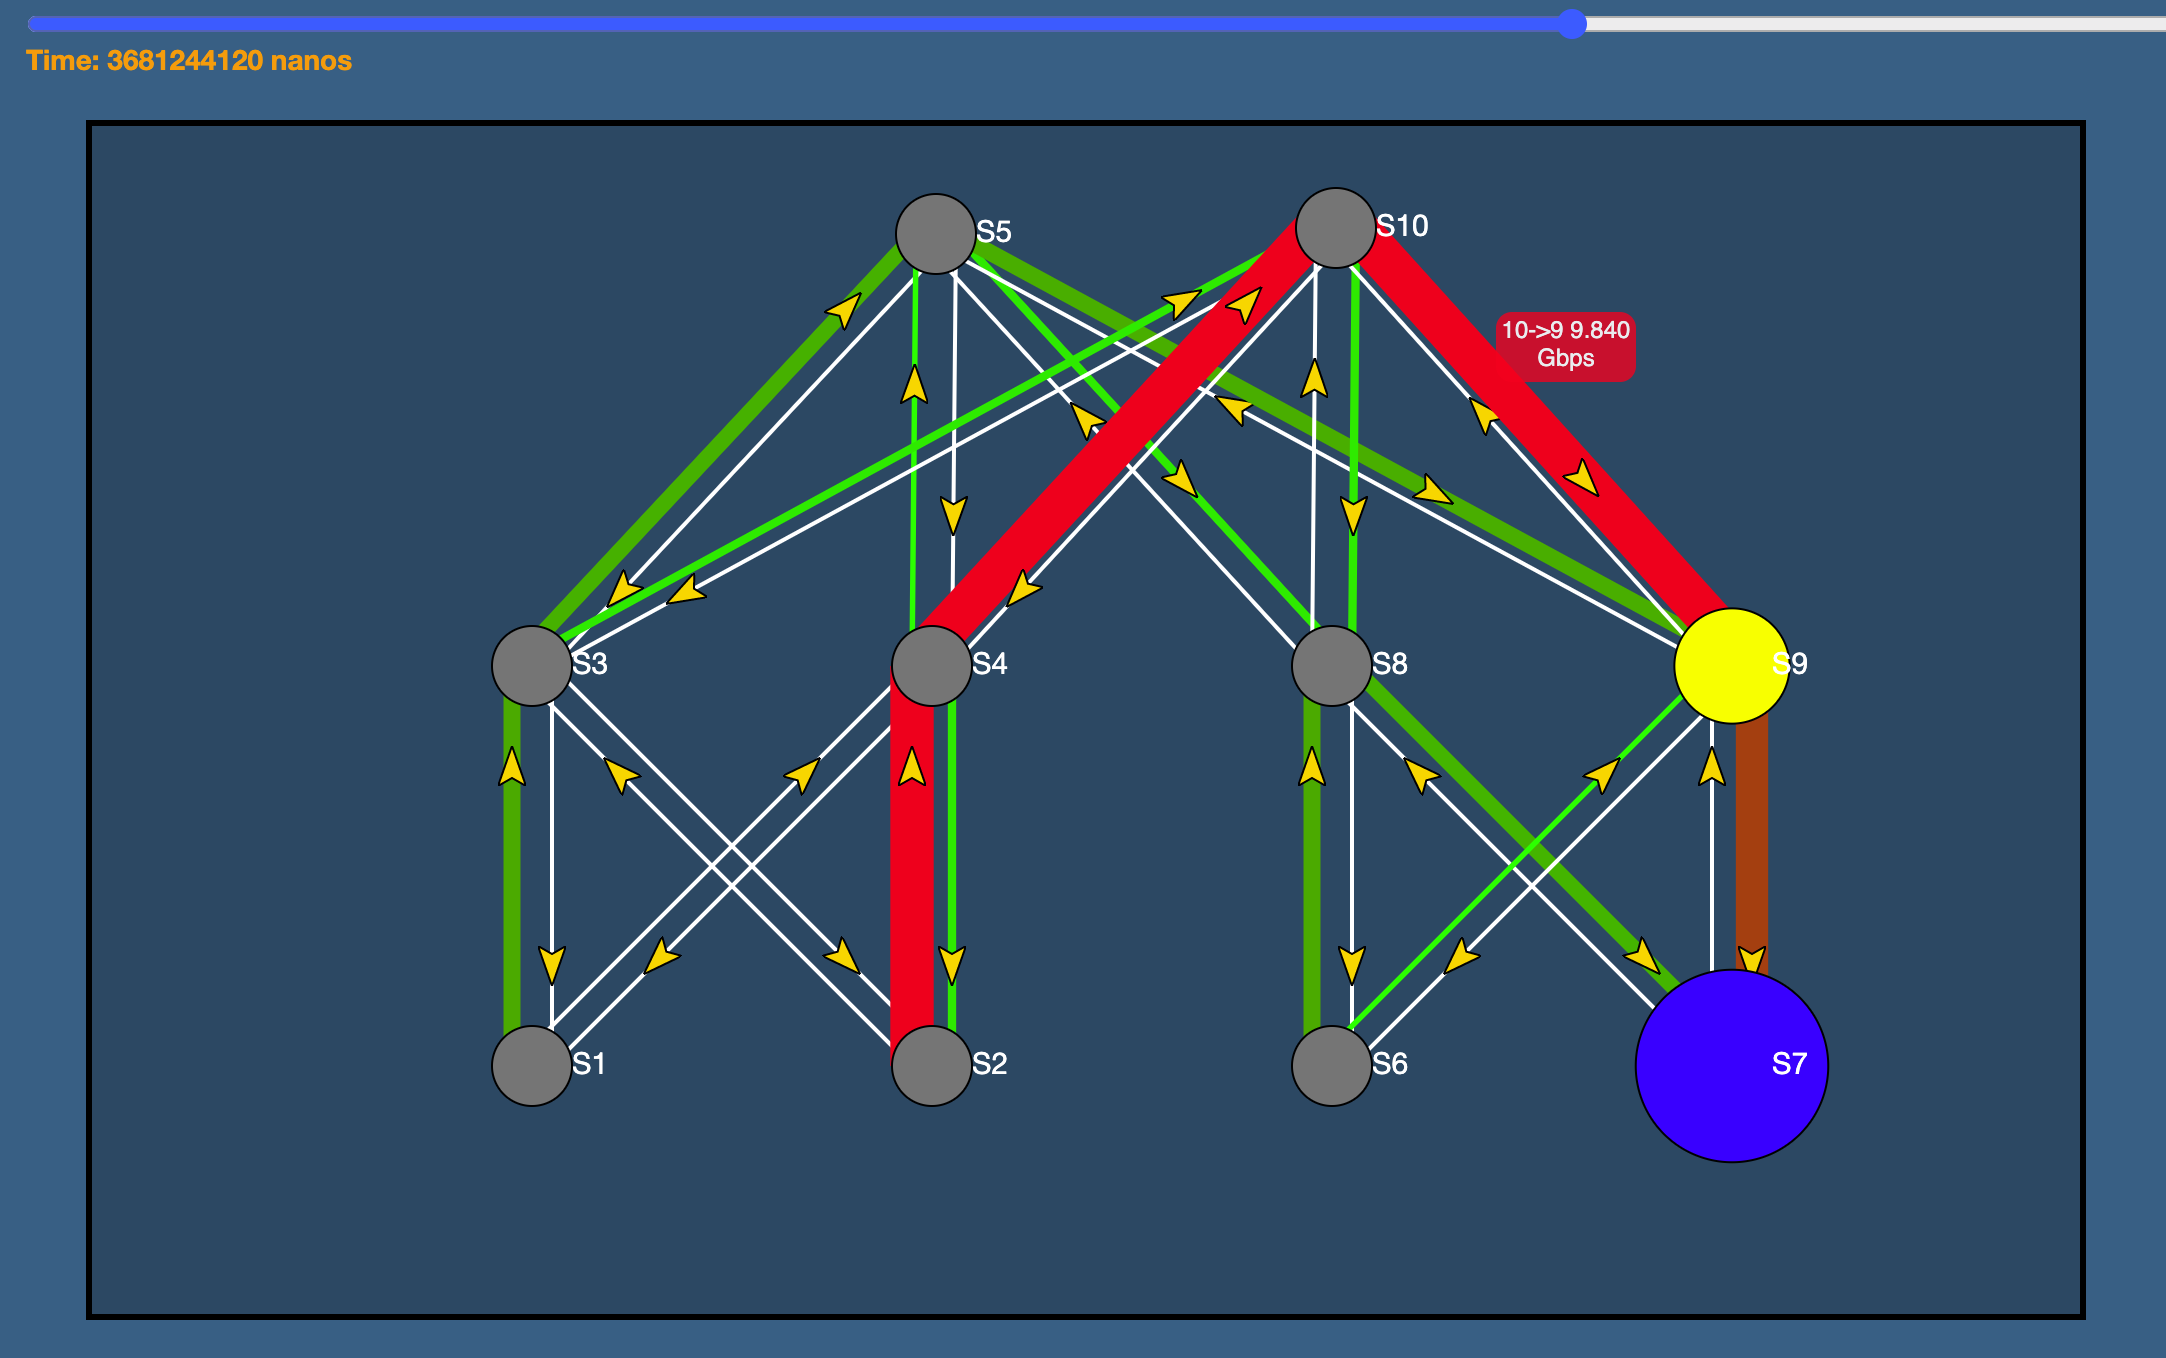
\includegraphics[width=1.0\columnwidth]{Figures/egress_example.png}
		\rule{35em}{0.5pt}
	\caption[Link Throughputs Visualizations]{An example of how powerful visualizations can be created with this quantity. The thick red link indicates existence of a heavy hitter flow dude to very high throughput. Then enlarged blue switch indicates buildup of queue in the switch.}
	\label{fig:Eg_example}
\end{figure}
%% Chapter Template

\chapter{Demonstration and Debugging of sample scenarios} % Main chapter title

\label{Chapter5} % Change X to a consecutive number; for referencing this chapter elsewhere, use \ref{ChapterX}

\lhead{Chapter 5. \emph{Demonstration and debugging of sample scenarios}} % Change X to a consecutive number; this is for the header on each page - perhaps a shortened title

%----------------------------------------------------------------------------------------
%	SECTION 1
%----------------------------------------------------------------------------------------

This chapter is intended to demonstrate how a combination of relational data as well as the created
visualizations can help a network administrator to the state and understand the fault in the network.

We look at the following two problems here: The synchronous incast problem and the asynchronousincast problem.

\section{The Synchronous Incast Problem}

\subsection{Description}

This type of problem occurs in data centers in applications like MapReduce and DFS exhibiting fan-in traffic patterns.
This occurs when multiple hosts send data to a single host. In the case where the traffic from multiple hosts is
synchronized(common in scatter-gather architectures, Figure \ref{fig:Synch Incast}), it may lead to heavy congestion for a short duration (of the
order of microseconds\cite{microburst}) and lead to spikes in queuing delay even when none of the flows are individually anywhere near
the capacity of the link.

\begin{figure}[htbp]
	\centering
		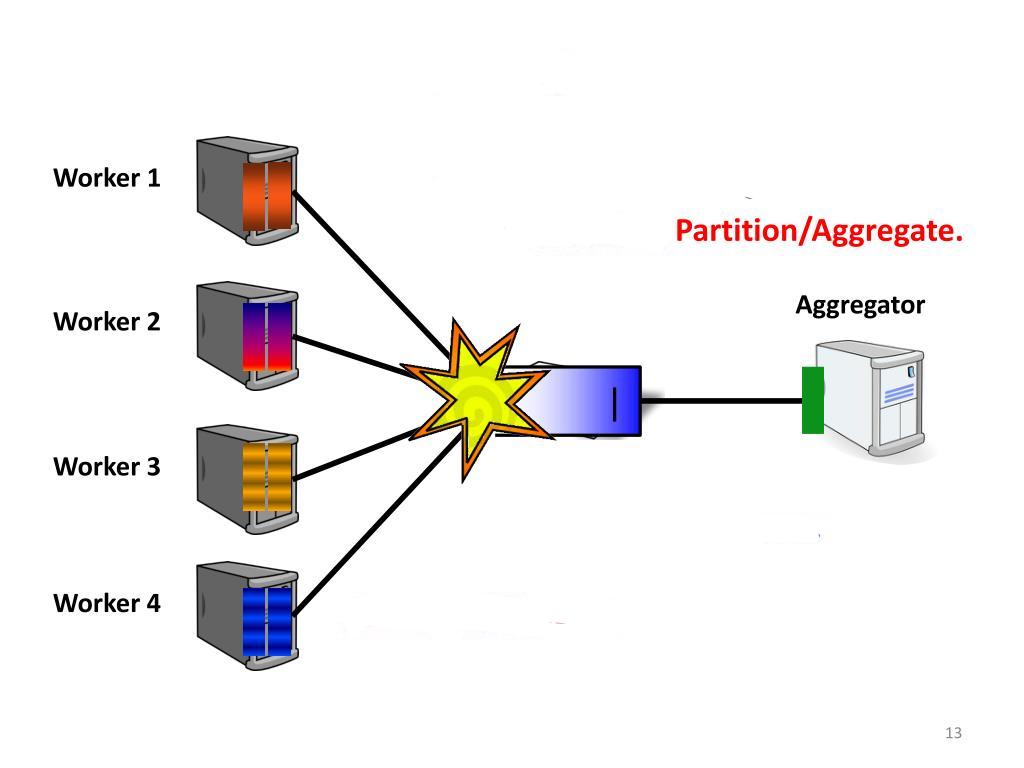
\includegraphics[width=0.65\columnwidth]{Figures/sync_incast.jpg}
		\rule{35em}{0.5pt}
	\caption[Synchronized Incast]{Synchronized Incast in Partition-Aggregate architecture}
	\label{fig:Synch Incast}
\end{figure}

\subsection{Configuration}
For creating a synchronized incast scenario in our topology, we generate traffic of 1 Gbps from hosts H1 to H6. The flow are routed
according to Figure \ref{fig:Synch Incast Topo} and get aggregated at switch 7.
\begin{figure}[htbp]
	\centering
		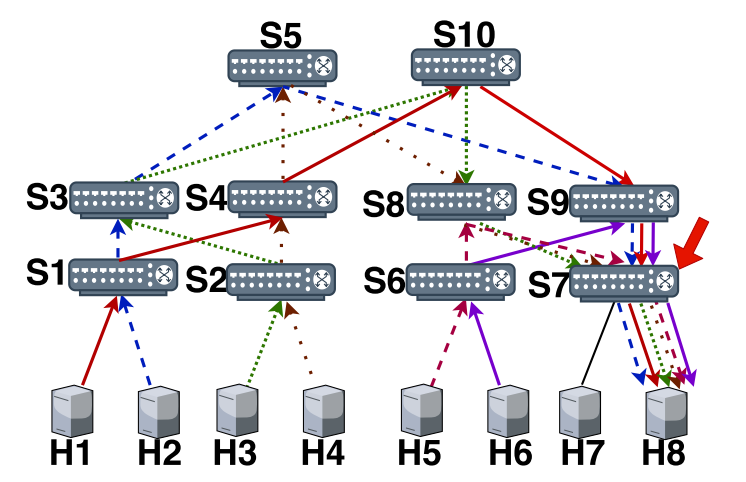
\includegraphics[width=0.65\columnwidth]{Figures/sync_incast_topo.png}
		\rule{35em}{0.5pt}
	\caption[Synchronized Incast Flows]{Synchronized Incast at switch 7 due to synchronized Fan-in traffic}
	\label{fig:Synch Incast Topo}
\end{figure}


\subsection{Diagnosis}
A synchronized microburst will often lead to multiple spikes occuring in a plot 
of the queue depth at the trigger switch. An algorithm for determining the width of
the peak queueDepth is described here.

\begin{algorithm}
	\caption{Estimate Width of Peak}
	\begin{algorithmic}[1]
		\REQUIRE indexOfPeak, records, peakDepth
		\STATE $leftThreshold \leftarrow 0.3, rightThreshold \leftarrow 0.5$
		\STATE $leftIndex = indexOfPeak - 1$
		\STATE $rightIndex = indexOfPeak + 1$
		% \WHILE{$leftIndex \geq 0$}
		
		\WHILE{$records[leftIndex].depth \geq leftThreshold \times peakDepth$}
		\STATE $leftIndex = leftIndex - 1$
		\ENDWHILE

		\WHILE{$records[rightIndex].depth \geq rightThreshold \times peakDepth$}
		\STATE $rightIndex = rightIndex + 1$
		\ENDWHILE

		\STATE $width = records[rightIndex].timeOut - records[leftIndex].timeIn$
		% \ENDWHILE
		% }
	\end{algorithmic}
\end{algorithm}

Once the peak is estimated, we look at the distribution of packets that came into the queue during the peak
as well as the packets that were present in the queue at the start of the peak.
We use Jain's Fairness Index (Appendix \ref{AppendixA}) to estimate fairness of distribution of packets according to source IP.
If the Jain's Fairness Index turns out to be greater than a predetermined threshold of 0.7, then it is classified as a case of 
Synchronized Incast due to the observation that in a synchronized incast, the distribution of packets is mostly fair.
\subsection{Results and Illustrations}
The above heuristic was applied in 5 different scenarios of synchronized incast of varied transmission rates.
The resultant values of Fairness Index calculated are given in table \ref{tab:J_Index_Sync}
\begin{table}[h]
\begin{center}
\begin{tabular}{ |p{3cm}|p{3cm}|  }
	\hline
	\multicolumn{2}{|c|}{Jain's Index} \\
	\hline
	Scenario & Value \\
	\hline
	1 & 0.957 \\
	2 & 0.980 \\
	3 & 0.890 \\
	4 & 0.780 \\
	5 & 0.975 \\
	\hline
   \end{tabular}
\end{center}

\caption{Jain's Index Values for different scenarios of Synchronous Incast}
% Help
\label{tab:J_Index_Sync}
\end{table}
The operator first looks at the readings of Jain's Index (Fig. \ref{fig:jind_sync} which point him towards the fact that it is a possible
case of synchronized incast.
Then he looks at the birds eye view of the network and seens that all flows seem to converge at the trigger switch at the same time (Fig. \ref{fig:genview_sync}).
Further, to help the network operator visualize the scenario, plots of queue depth at the
trigger switch are plotted, along with packet distribution in the estimated peak, as shown in figures \ref{fig:queue_depth_sync}
and \ref{fig:distribution_sync}.
The operator then looks at the plot of ingress throughput and concludes that all the flows entered the switch
at roughly the same time, and there is a certain periodicity in their arrival, as shown in Fig. \ref{fig:ing_sync}
These hints are enough to suggest to him that the problem is of a synchronous incast.

\begin{figure}[htbp]
	\centering
		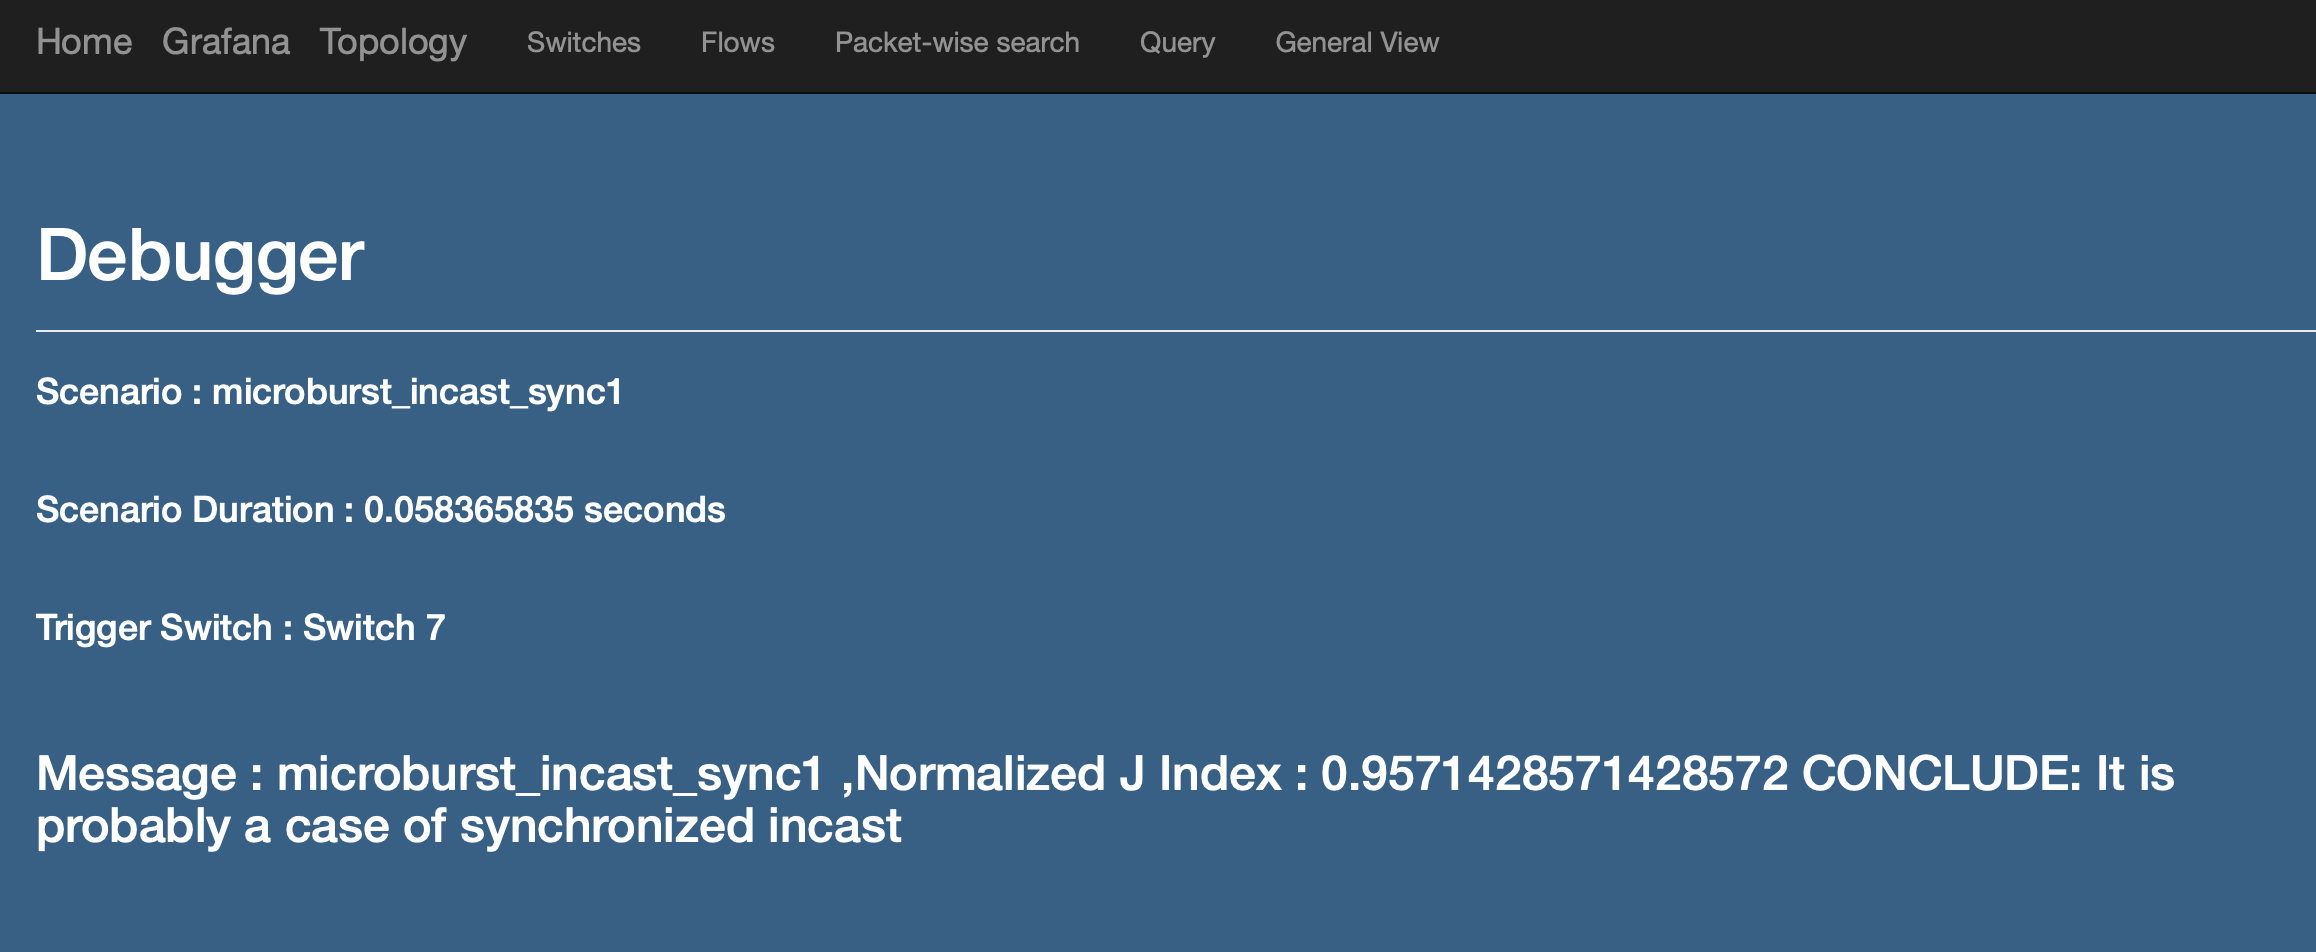
\includegraphics[width=1.0\columnwidth]{Figures/jindex_sync.png}
		\rule{35em}{0.5pt}
	\caption[Debugger Home Page, Synchronous Incast]{J Index calculated and presented to administrator}
	\label{fig:jind_sync}
\end{figure}

\begin{figure}[htbp]
	\centering
		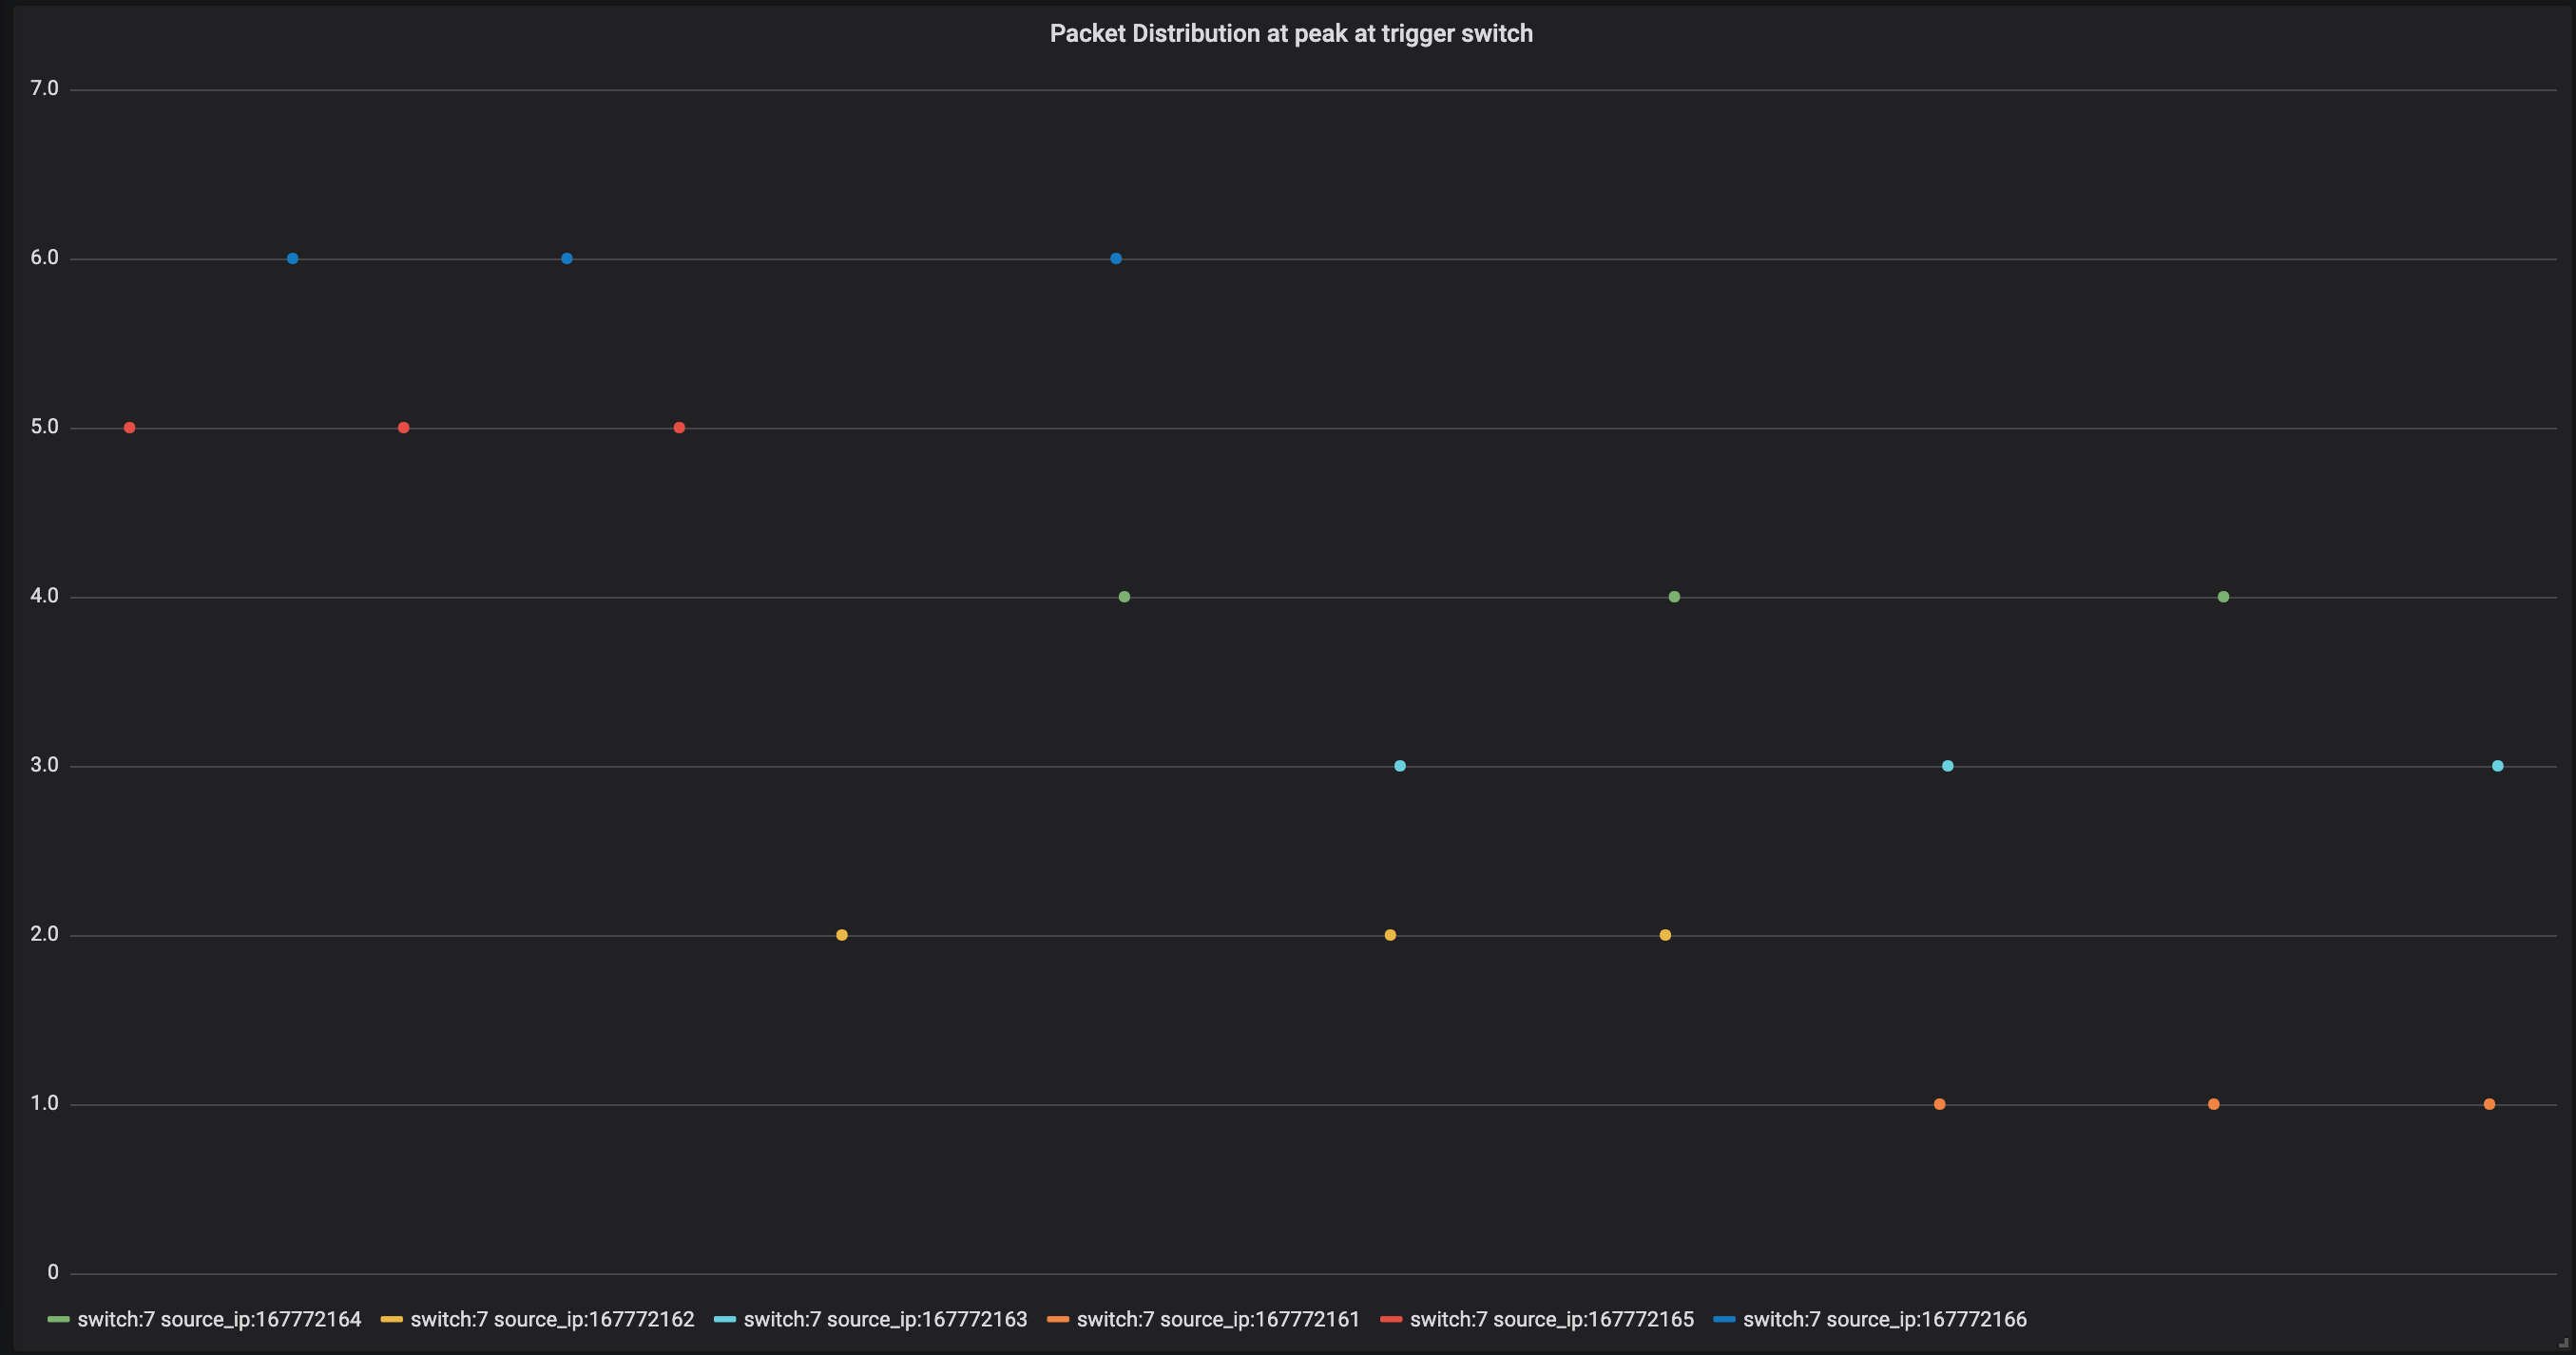
\includegraphics[width=1.0\columnwidth]{Figures/distribution_sync.png}
		\rule{35em}{0.5pt}
	\caption[Packet Distribution at Trigger Switch, Sync Incast]{Packet Distribution at Trigger Switch, Sync Incast. Note the highly even distribution.}
	\label{fig:distribution_sync}
\end{figure}

\begin{figure}[htbp]
	\centering
		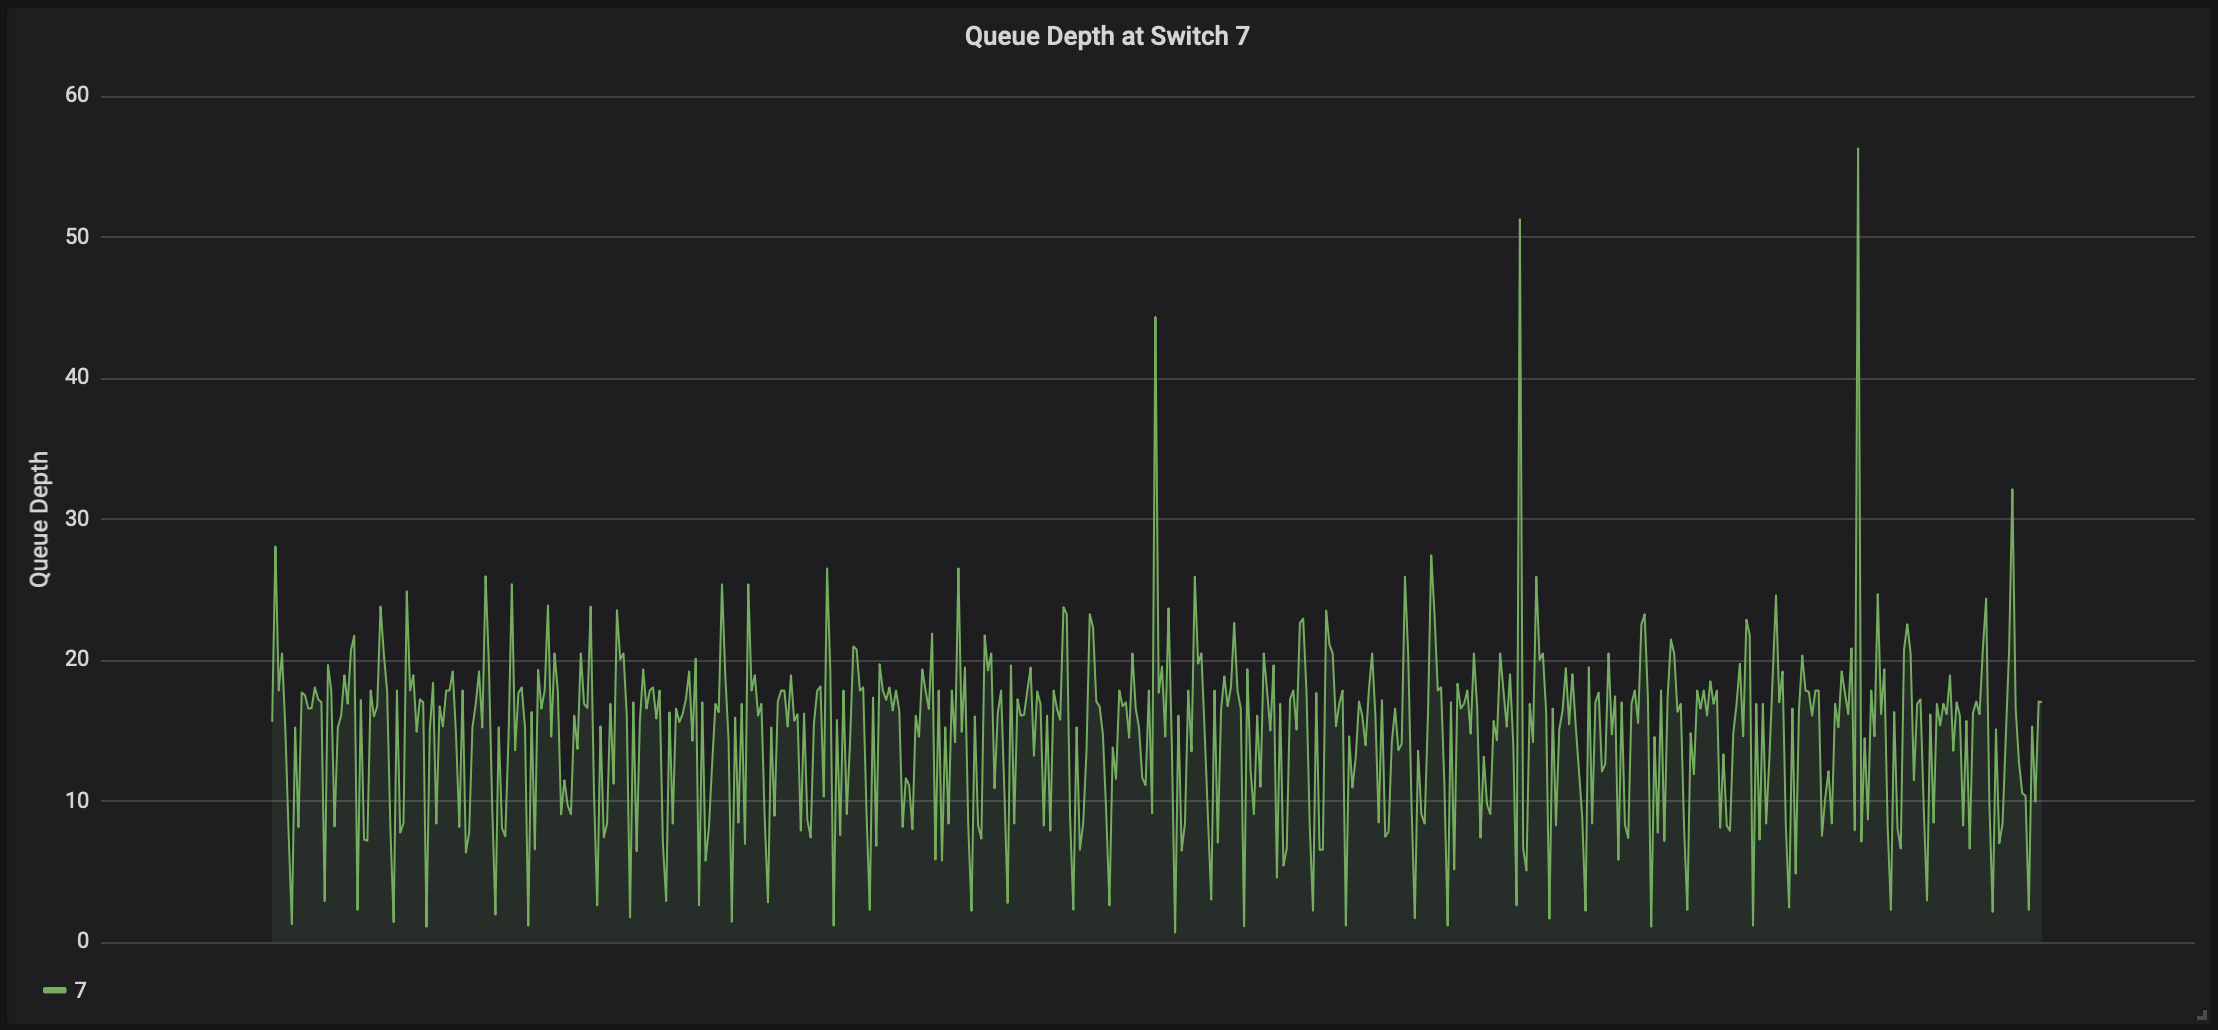
\includegraphics[width=1.0\columnwidth]{Figures/queue_depth_sync.png}
		\rule{35em}{0.5pt}
	\caption[Queue Depth at Trigger Switch, Sync Incast]{Queue Depth at Trigger Switch, Sync Incast}
	\label{fig:queue_depth_sync}
\end{figure}

\begin{figure}[htbp]
	\centering
		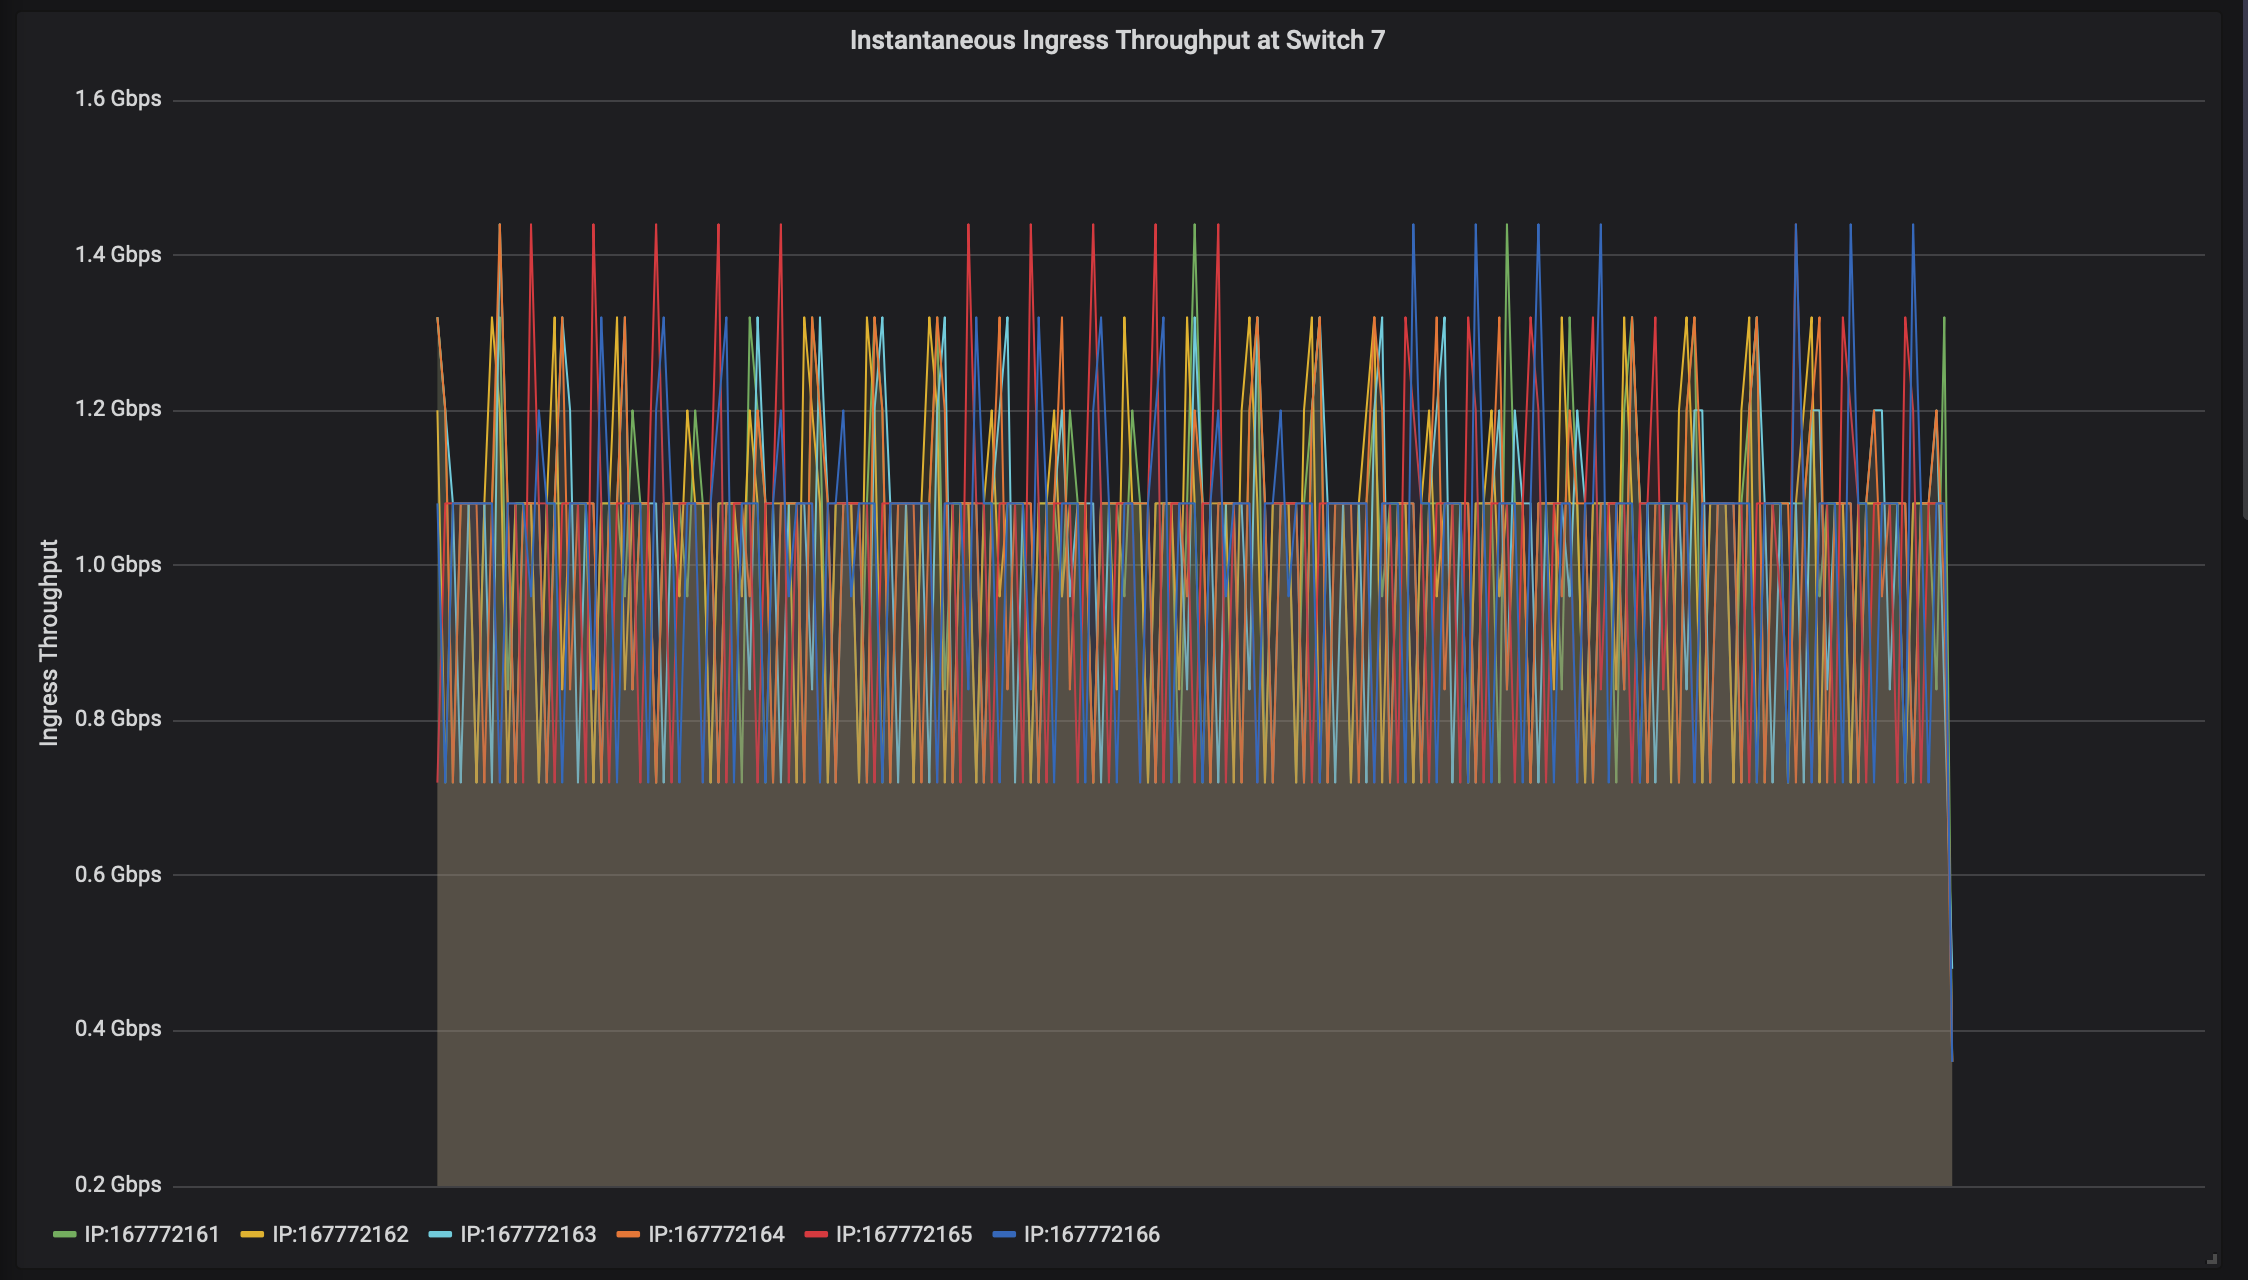
\includegraphics[width=1.0\columnwidth]{Figures/ingress_sync.png}
		\rule{35em}{0.5pt}
	\caption[Ingress Throughput for Synchronous Incast]{Ingress throughput for synchronous incast.}
	\label{fig:ing_sync}
\end{figure}

\begin{figure}[htbp]
	\centering
		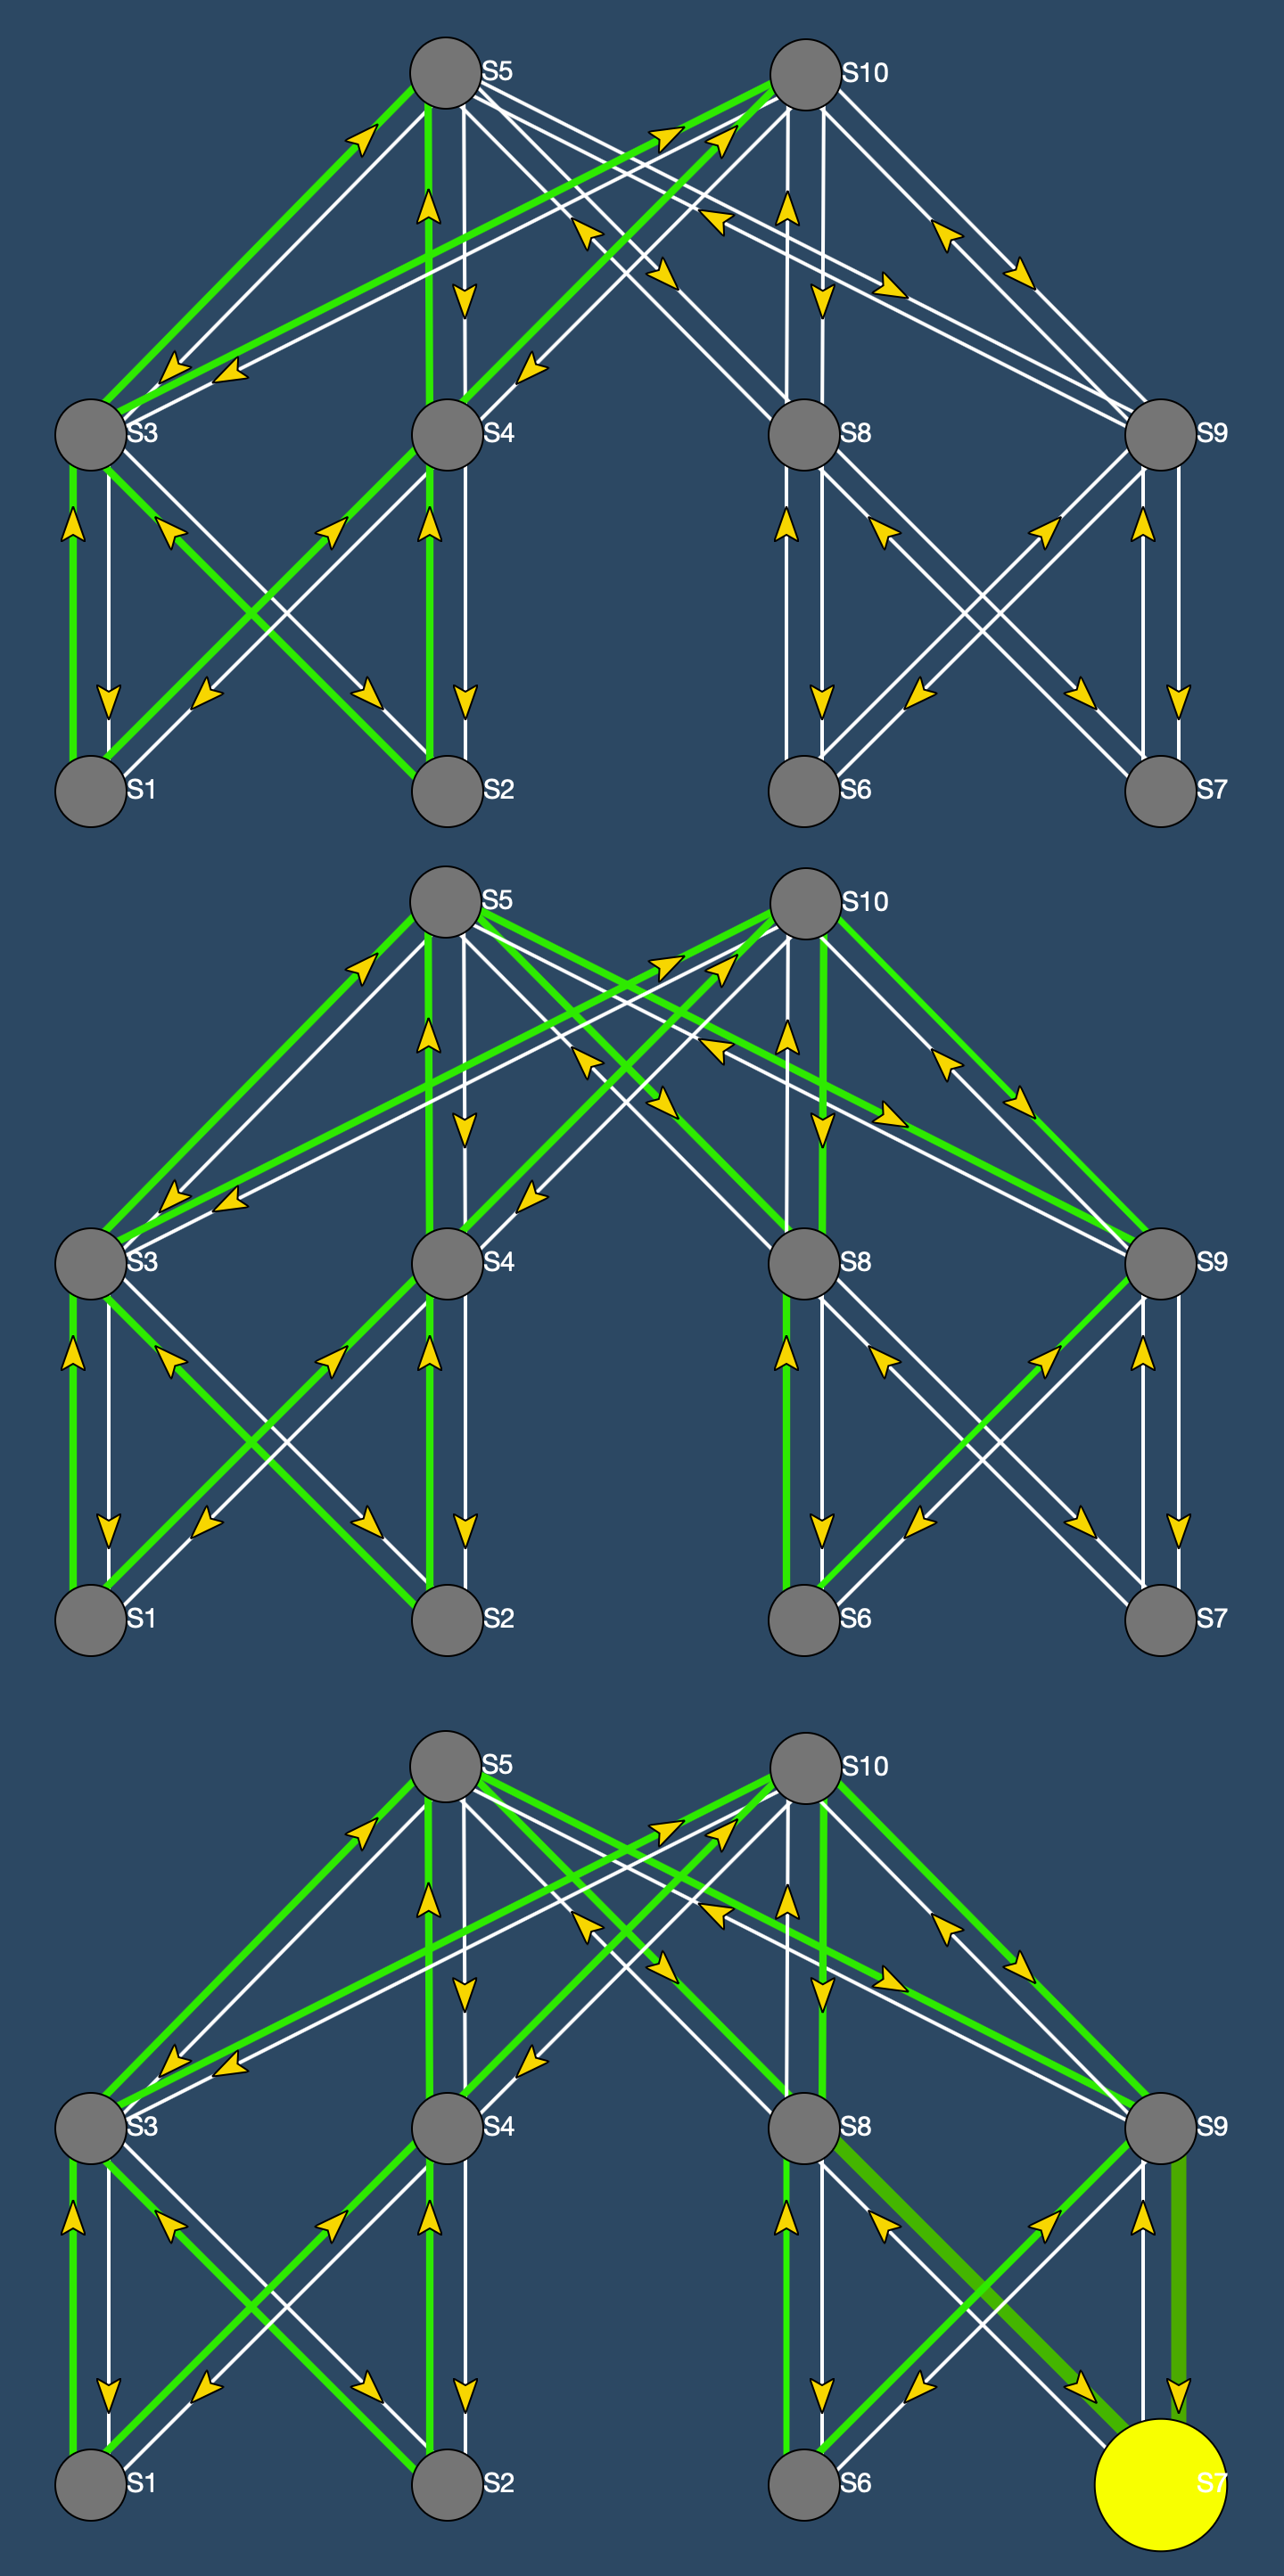
\includegraphics[width=20cm,height=25cm,keepaspectratio]{Figures/genview_sync.png}
		\rule{35em}{0.5pt}
	\caption[Birds eye view, Synchronous Incast]{Birds eye view of network at chronological points in time.}
	\label{fig:genview_sync}
\end{figure}

\section{Asynchronous Incast problem and Heavy Hitters}
\subsection{Description}
The Asynchronous Incast problem simply means a scenario where the queue depth increases over a period of microbursts
in the lack of any visible synchronization pattern. Often in these cases, we have the presence of a heavy hitter flow\cite{HH}
(A flow which consumes a substantial amount of bandwidth that violates fairness) which causes congestion and overflowing
of buffers in switch.
\subsection{Configuration}
For creating an asynchronous incast scenario in our topology, we generate traffic of 1 Gbps from H1, H3, H4 and 6 Gbps from H6. The flow are routed
according to Figure \ref{fig:Synch Incast Topo} and get aggregated at switch 7.
\subsection{Diagnosis}
In cases of asynchronous incast with heavy hitters, we will see a single large peak in the plot of queue depth and usually a very
skewed distribution in the peak. The heuristic used here is similar to the one in synchronous incast except if the Jain's 
Fairness Index is less that 0.45, then it is classified as an asynchronous incast problem.
\subsection{Results and Illustrations}

The above heuristic was applied in 5 different scenarios of aynchronous incast of varied transmission rates.
The resultant values of Fairness Index calculated are given in table \ref{tab:J_Index_Async}.
\begin{table}[h]
	\begin{center}
	\begin{tabular}{ |p{3cm}|p{3cm}|  }
		\hline
		\multicolumn{2}{|c|}{Jain's Index} \\
		\hline
		Scenario & Value \\
		\hline
		1 & 0.469 \\
		2 & 0.362 \\
		3 & 0.383 \\
		4 & 0.418 \\
		5 & 0.403 \\
		\hline
	   \end{tabular}
	\end{center}
	
	\caption{Jain's Index Values for different scenarios of Asynchronous Incast}
	% Help
	\label{tab:J_Index_Async}
	\end{table}

	The operator first looks at the readings of Jain's Index (Fig. \ref{fig:jind_async} which point him towards the fact that it is a possible
	case of asynchronized incast.
	Then he looks at the birds eye view of the network and seens that there is an interval of time when the links along a path fill up
	with traffic. (Fig. \ref{fig:genview_async}).
	Further, to help the network operator visualize the scenario, plots of ingress throughput and compositon of queue depth at 
	trigger switch are plotted, along with packet distribution in the estimated peak, as shown in figures \ref{fig:ing_throughput_async}, \ref{fig:queue_comp_async}
	and \ref{fig:distribution_async}
	Looking at the plot of ingress throughput, the operator sees that there is one heavyhitter flow with a rough throughputof 8 Gbps existing in the network.
	He also looks at the composition of the queue depth to see that a large number of packets at the peak are of the green flow (the heavy hitter).

	These hints suggest a case of asynchronous incast.

	\begin{figure}[htbp]
		\centering
			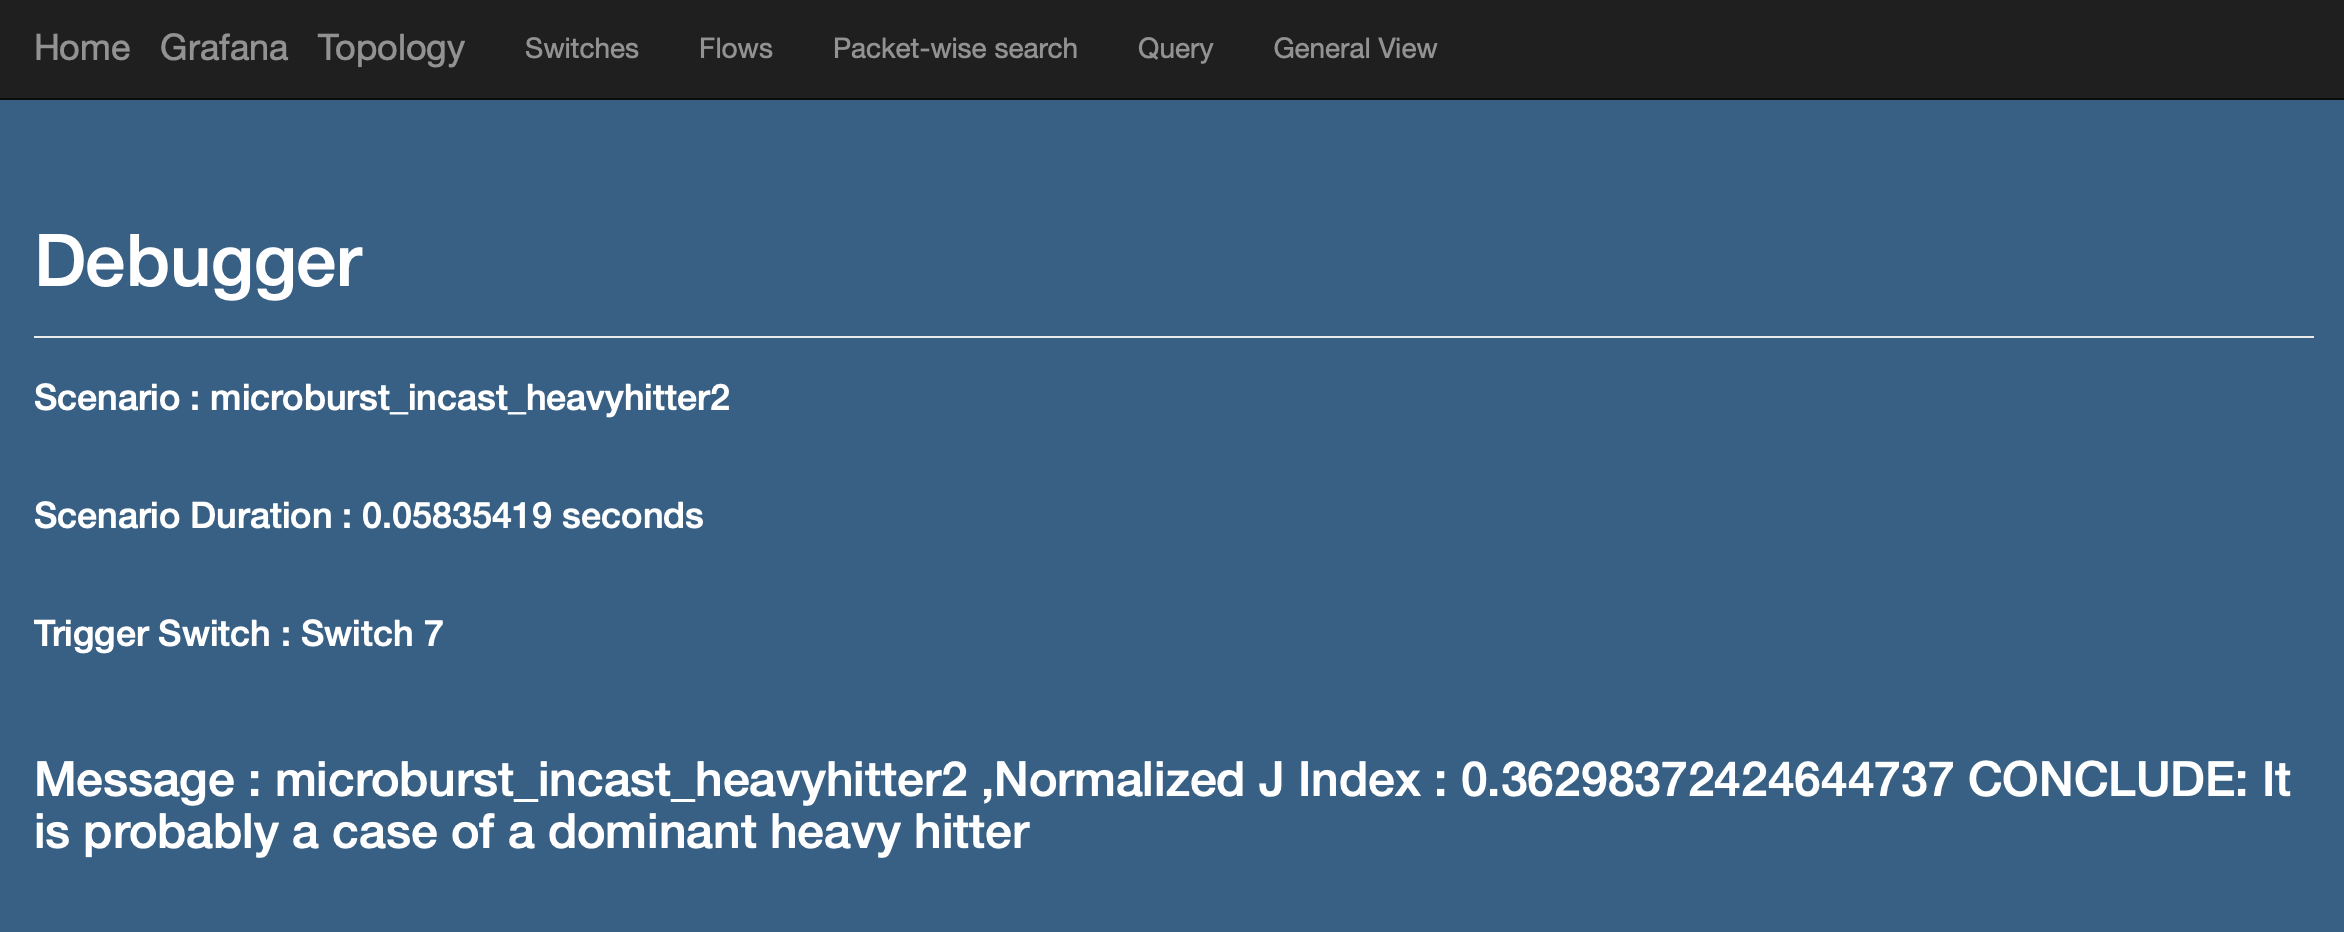
\includegraphics[width=1.0\columnwidth]{Figures/jindex_async.png}
			\rule{35em}{0.5pt}
		\caption[Debugger Home Page, Asynchronous Incast]{J Index calculated and presented to administrator}
		\label{fig:jind_async}
	\end{figure}

\begin{figure}[htbp]
	\centering
		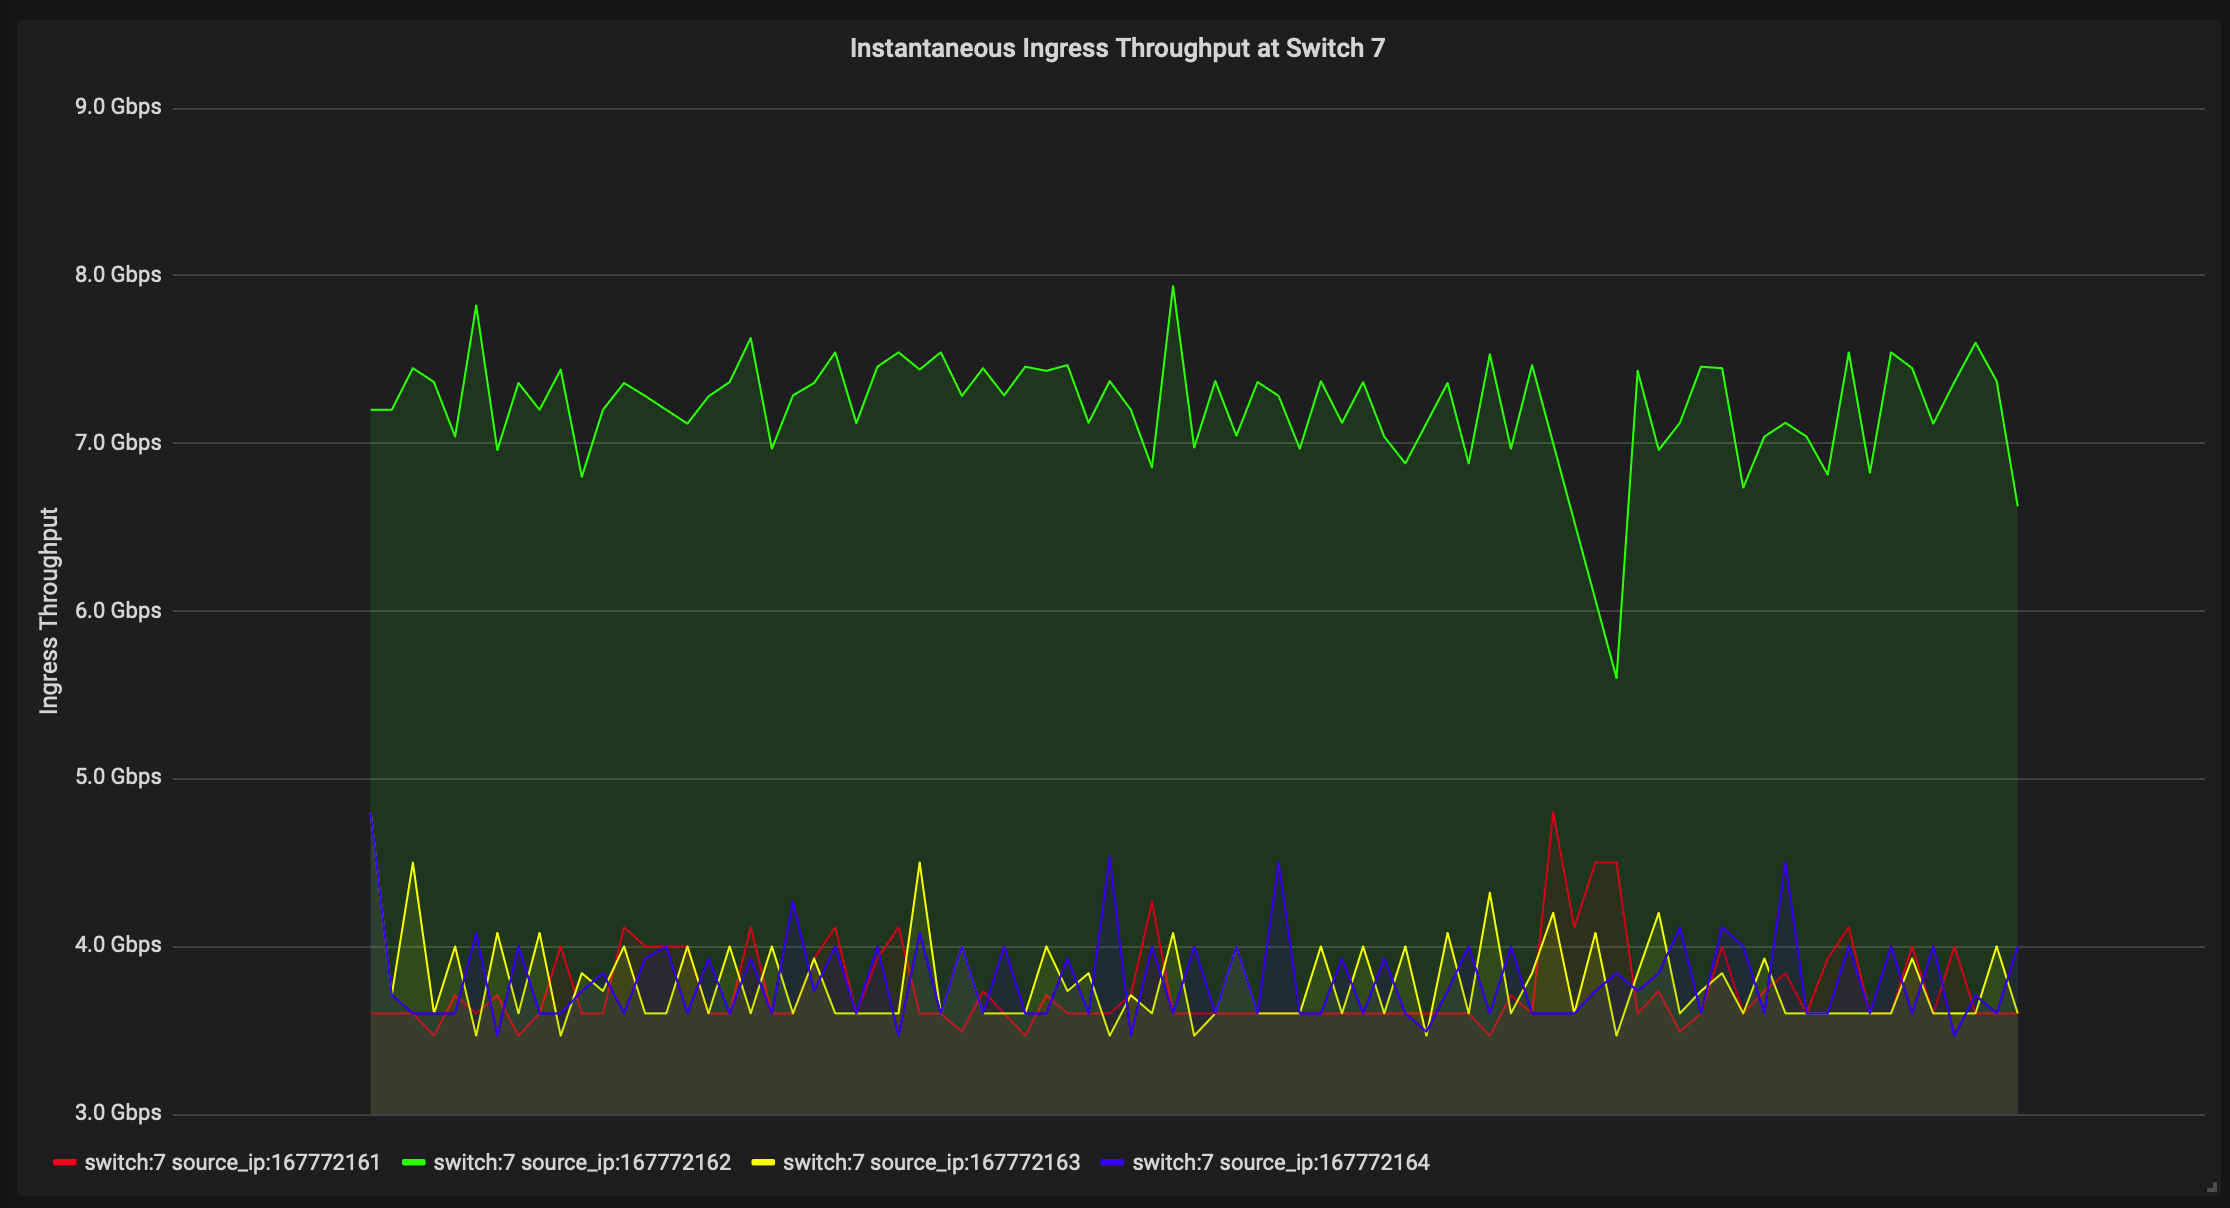
\includegraphics[width=1.0\columnwidth]{Figures/ing_thpt_async.png}
		\rule{35em}{0.5pt}
	\caption[Ingress Throughput Asynchronous Incast]{Ingress throughput for asynchronous incast}
	\label{fig:ing_throughput_async}
\end{figure}

\begin{figure}[htbp]
	\centering
		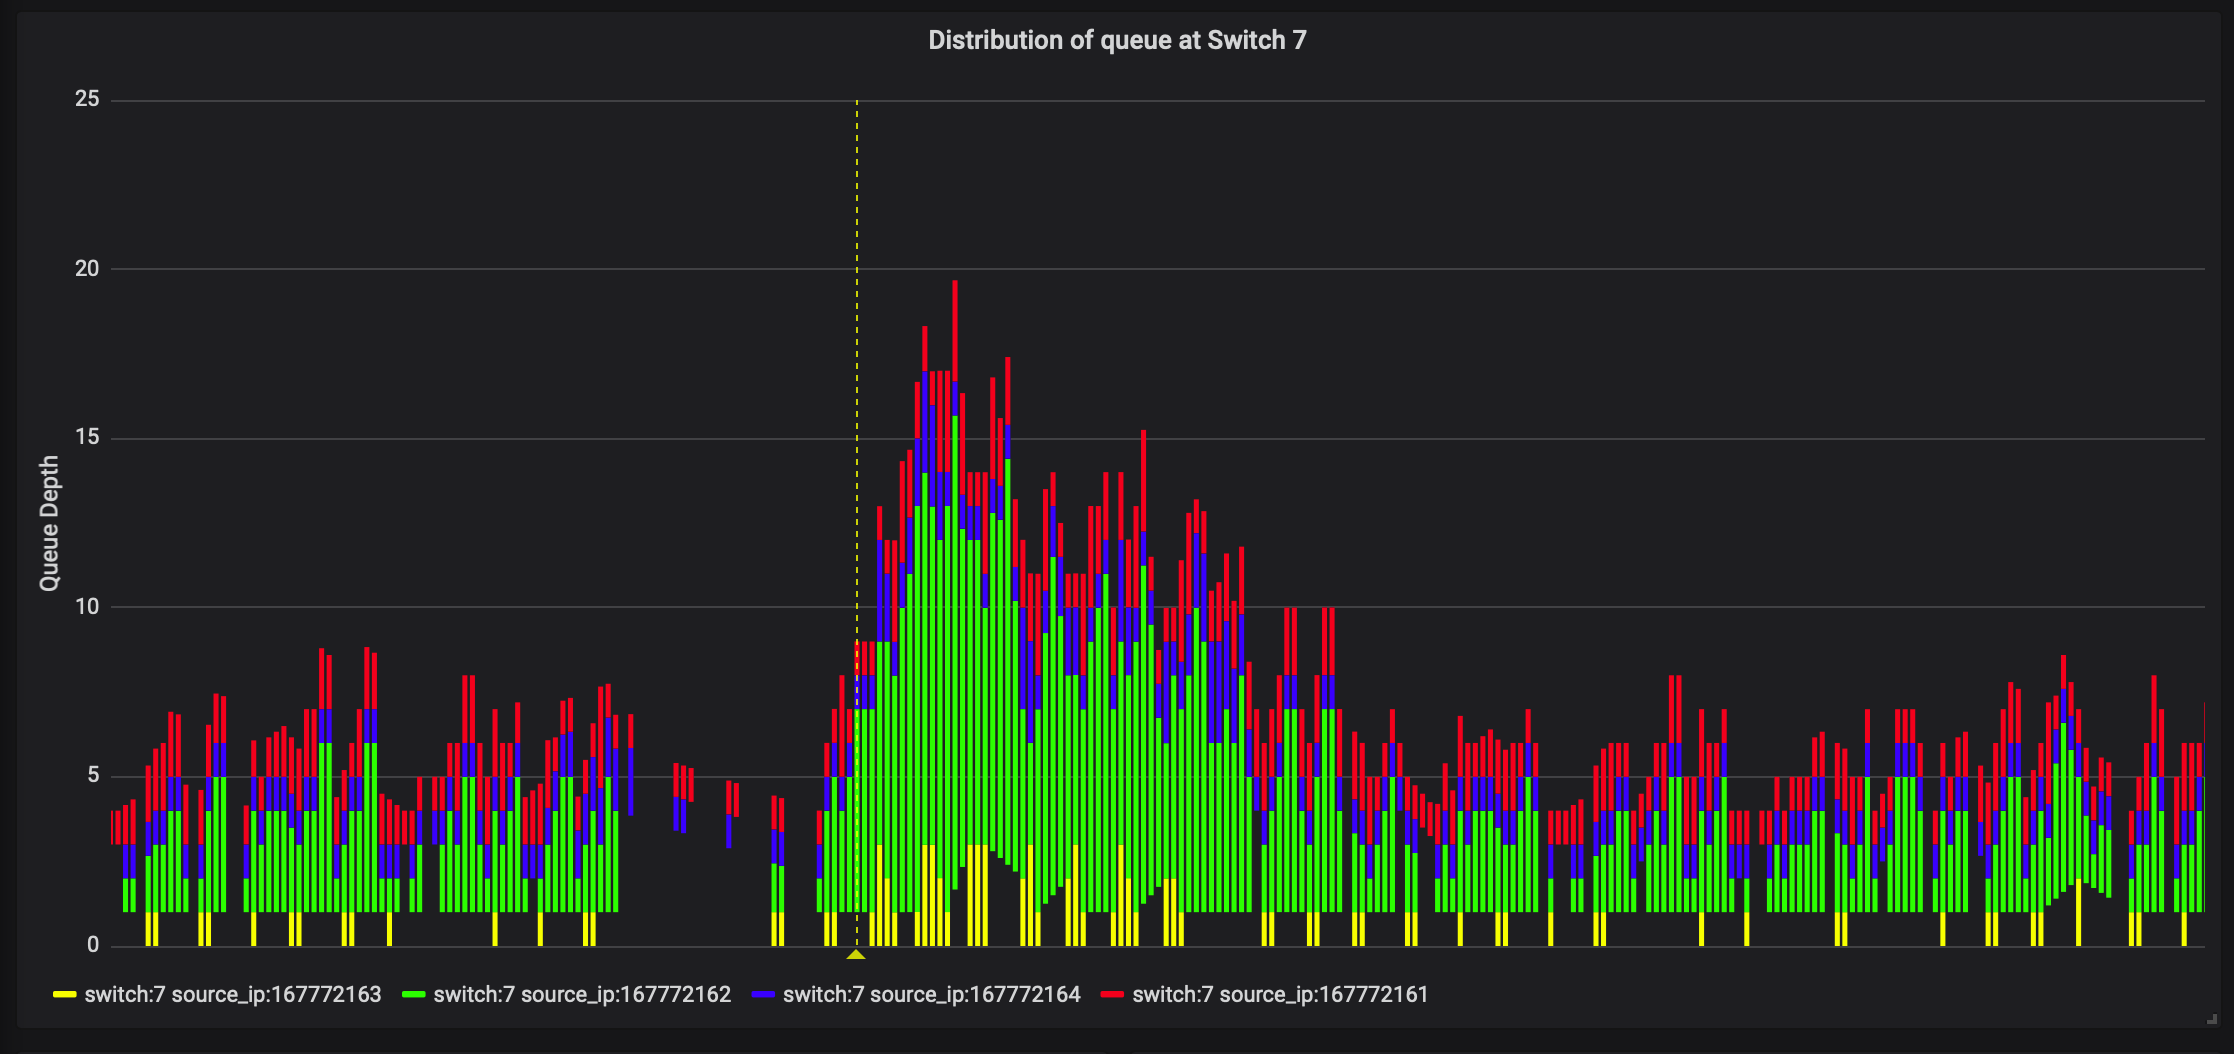
\includegraphics[width=1.0\columnwidth]{Figures/queue_comp_async.png}
		\rule{35em}{0.5pt}
	\caption[Queue Composition at Trigger Switch, Async Incast]{Queue Composition at Trigger Switch, Async Incast}
	\label{fig:queue_comp_async}
\end{figure}
\begin{figure}[htbp]
	\centering
		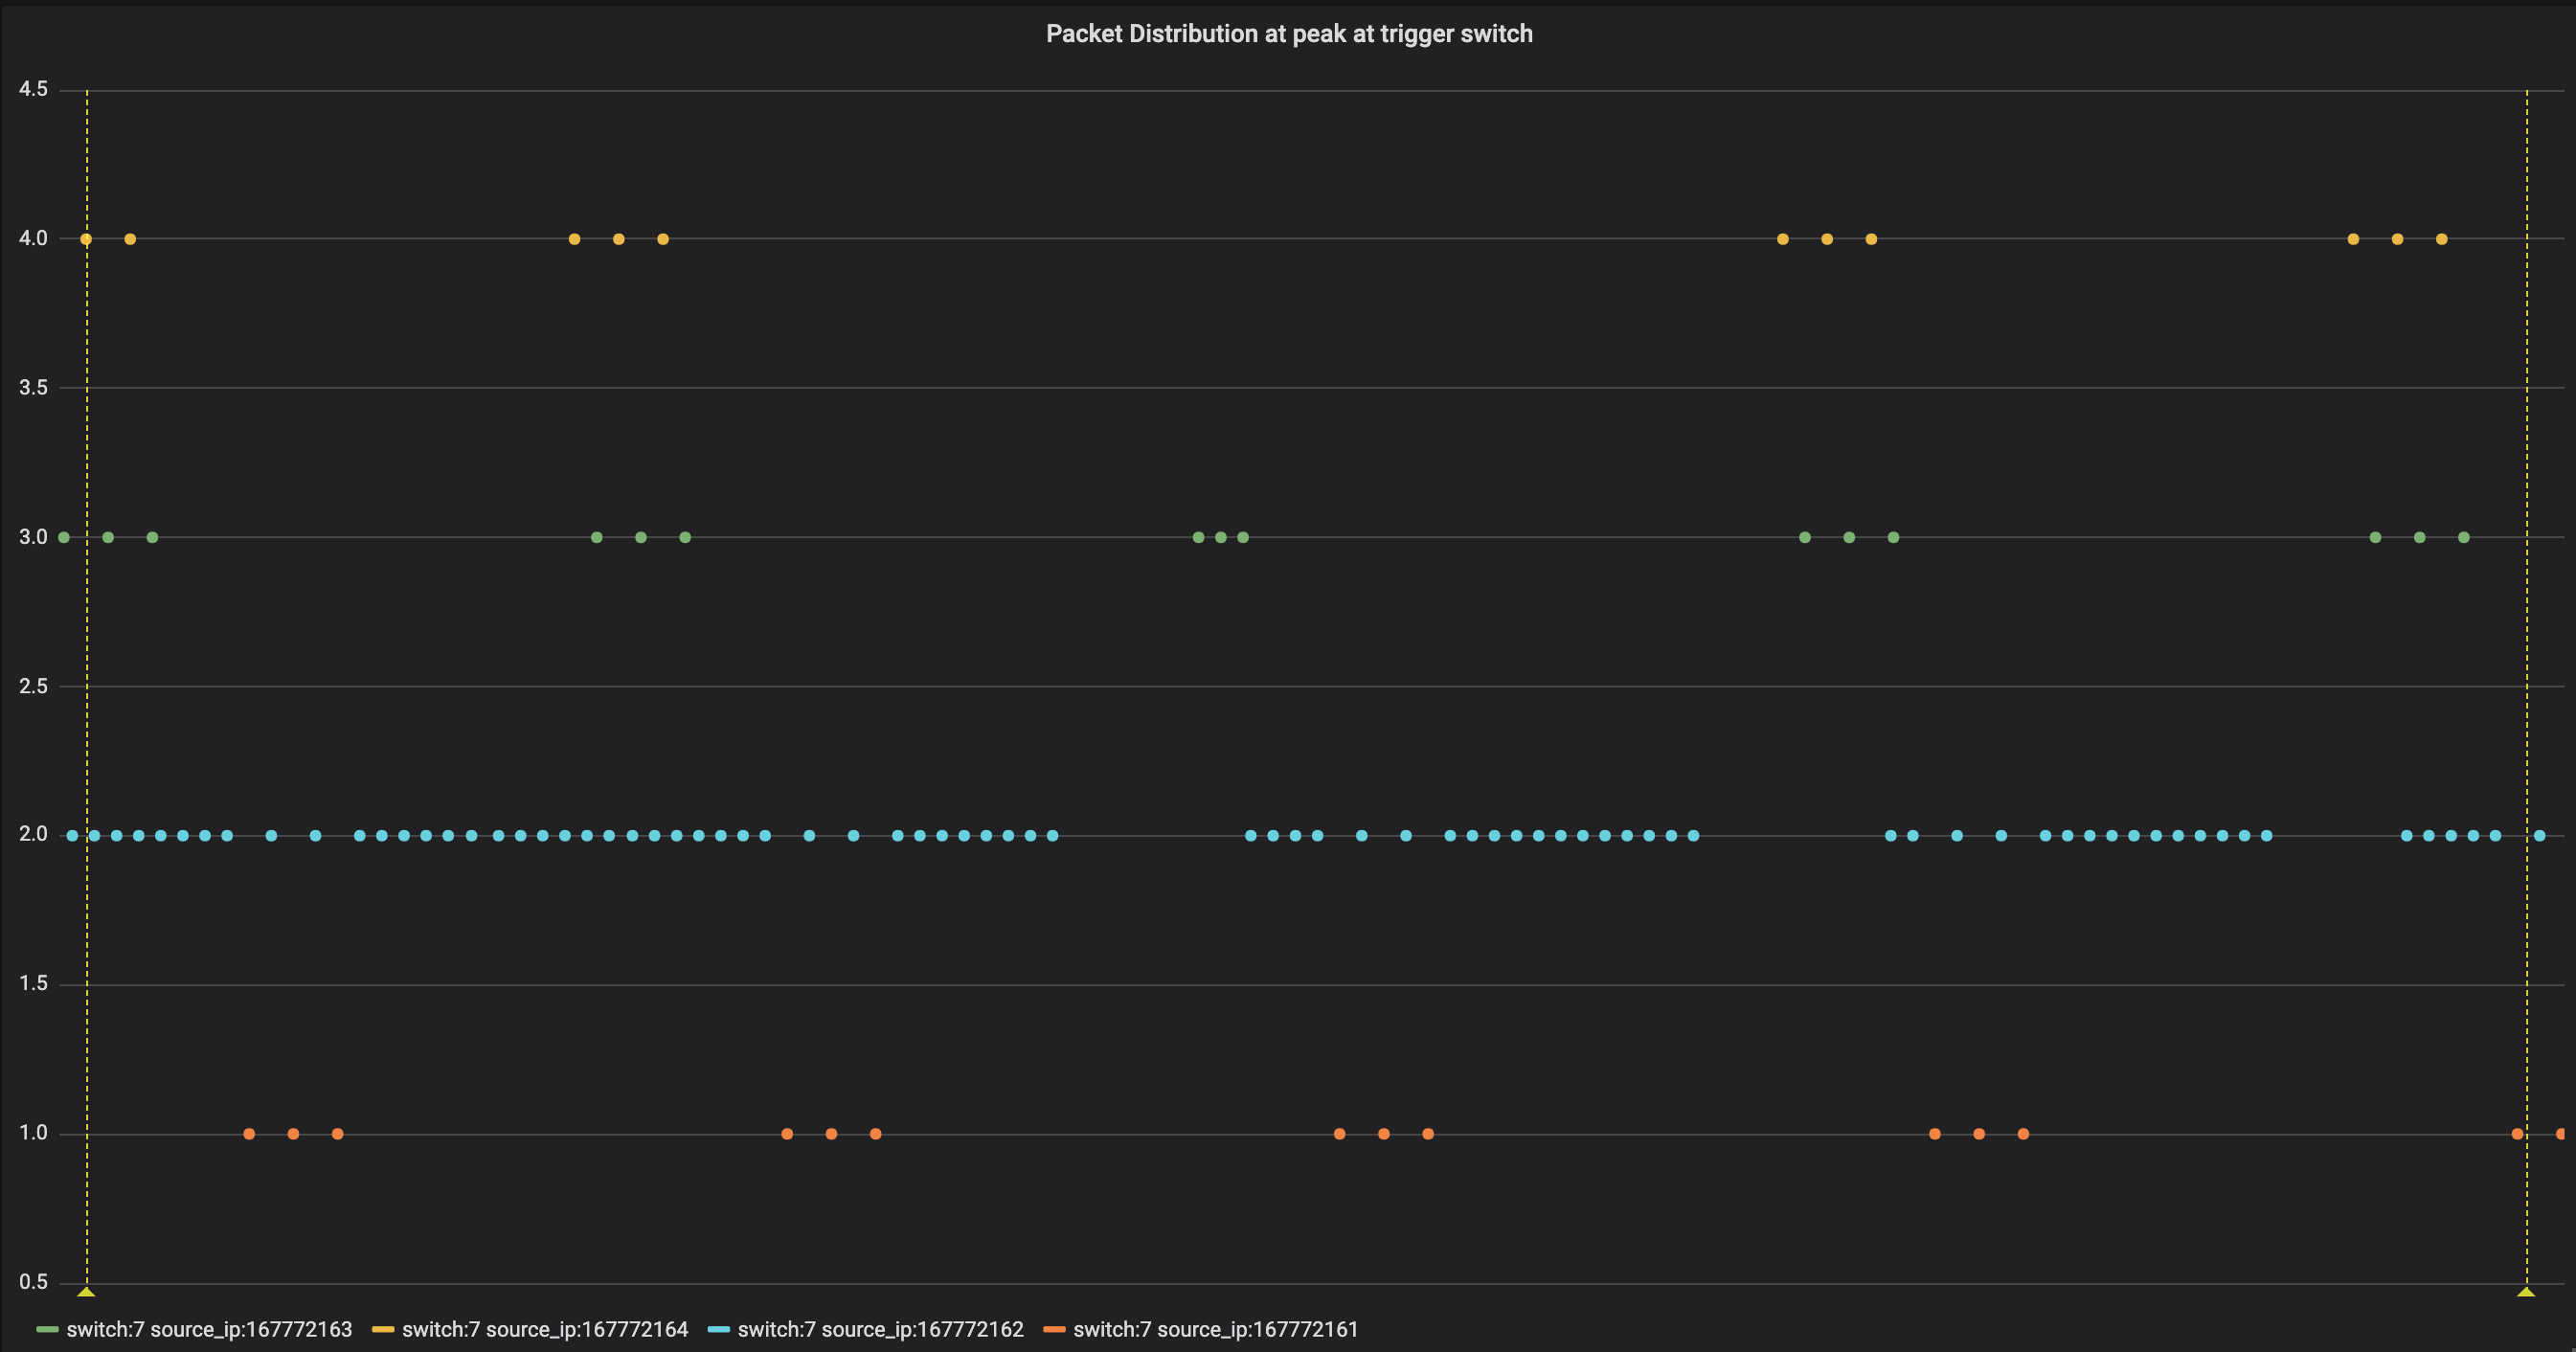
\includegraphics[width=1.0\columnwidth]{Figures/distribution_async.png}
		\rule{35em}{0.5pt}
	\caption[Packet Distribution at Trigger Switch, Async Incast]{Packet Distribution at Trigger Switch, Async Incast. Note the highly skewed distribution.}
	\label{fig:distribution_async}
\end{figure}

\begin{figure}[htbp]
	\centering
		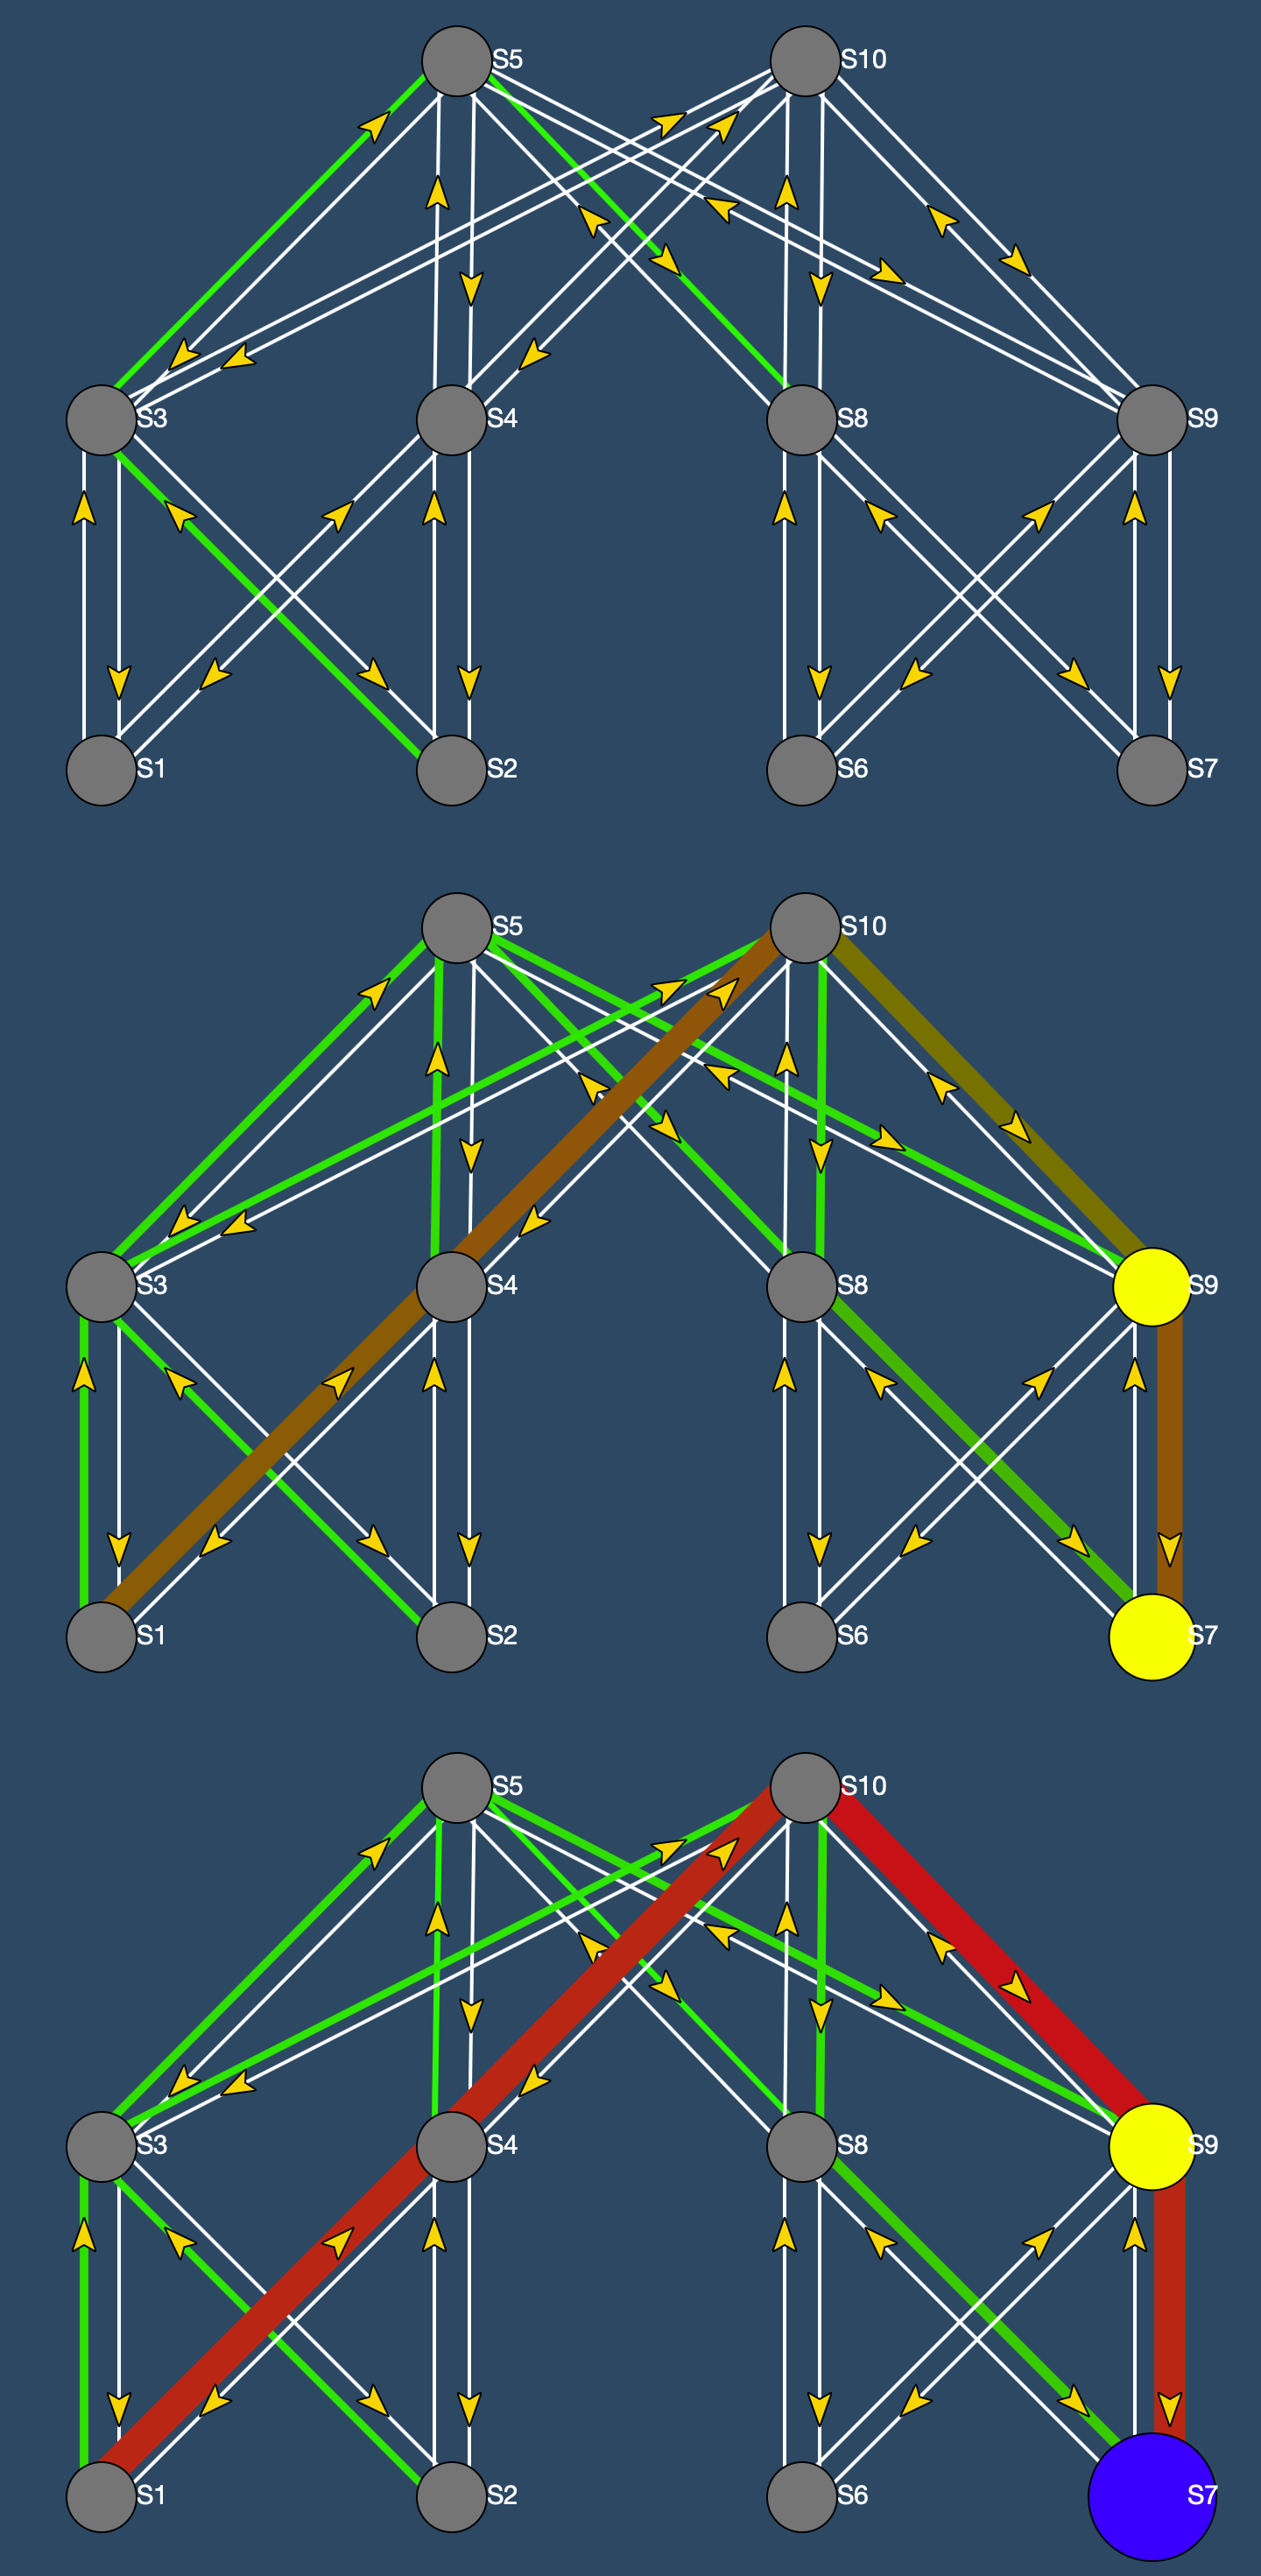
\includegraphics[width=20cm,height=25cm,keepaspectratio]{Figures/genview_async.png}
		\rule{35em}{0.5pt}
	\caption[Birds eye view, Asynchronous Incast]{Birds eye view of network at chronological points in time.}
	\label{fig:genview_async}
\end{figure}


\section{Link Underprovisioning}
\subsection{Description}
A link underprovision occurs when the link is operating at near, or maximum capacity for prolonged periods of time (of the order of milliseconds or seconds).
This usually requires the operator to provide additional bandwidth for the link.
It also leads to large buildup of queues in switches for prolonged periods of time.
\subsection{Configuration}
For creating a link underprovision scenario in our topology, we generate traffic of 6 Gbps from H3, H4, H5 and 1 Gbps from H1 and H2. The flow are routed
according to Figure \ref{fig:Synch Incast Topo} and get aggregated at switch 7.
\subsection{Diagnosis}
As stated before, a link will be underprovisioned if it is overutilized for a duration of the order of milliseconds.
If we find that the width of the peak as found in Algorithm 1 is of the order of milliseconds, and that the link is being overutilized, say by setting a threshold
to be average utilization greater than 0.8 * max capacity, then we classify the link to be overutilized.
\subsection{Results and Illustrations}
The above heuristic was applied to 2 different scenarios of link underprovision of varied transmission rates.
The resultant values of peak width calculated are given in table \ref{tab:Peak_Width}
\begin{table}[h]
\begin{center}
\begin{tabular}{ |p{3cm}|p{5cm}|  }
	\hline
	\multicolumn{2}{|c|}{Peak Width} \\
	\hline
	Scenario & Duration (in microseconds) \\
	\hline
	1 & 2575.626 \\
	2 & 4713.071 \\
	\hline
   \end{tabular}
\end{center}

\caption{Peak Width Duration for different scenarios of Link Underprovisioning}
% Help
\label{tab:Peak_Width}
\end{table}

The operator first looks at the recommendation given by the application as to what the fault is (Fig. \ref{fig:home_under}).
The operator looks at the birds eye view of the network and seens that there is massive buildup of queues along with maximum
capacity utilization of links.(Fig. \ref{fig:genview_under}).
Further, to help the network operator visualize the scenario, plots of ingress throughput and compositon of queue depth at 
trigger switch are plotted as shown in figures \ref{fig:ing_throughput_under} and \ref{fig:queue_comp_async}.
Looking at the plot of ingress throughput, the operator sees that there are two heavyhitter flows existing in the network.
He also looks at the composition of the queue depth to see that a large number of packets at the peak belong to these two flows and
that the queue only starts to buildup once these flows start entering the switch.

These hints suggest a case of underprovisioned network.

\begin{figure}[htbp]
	\centering
		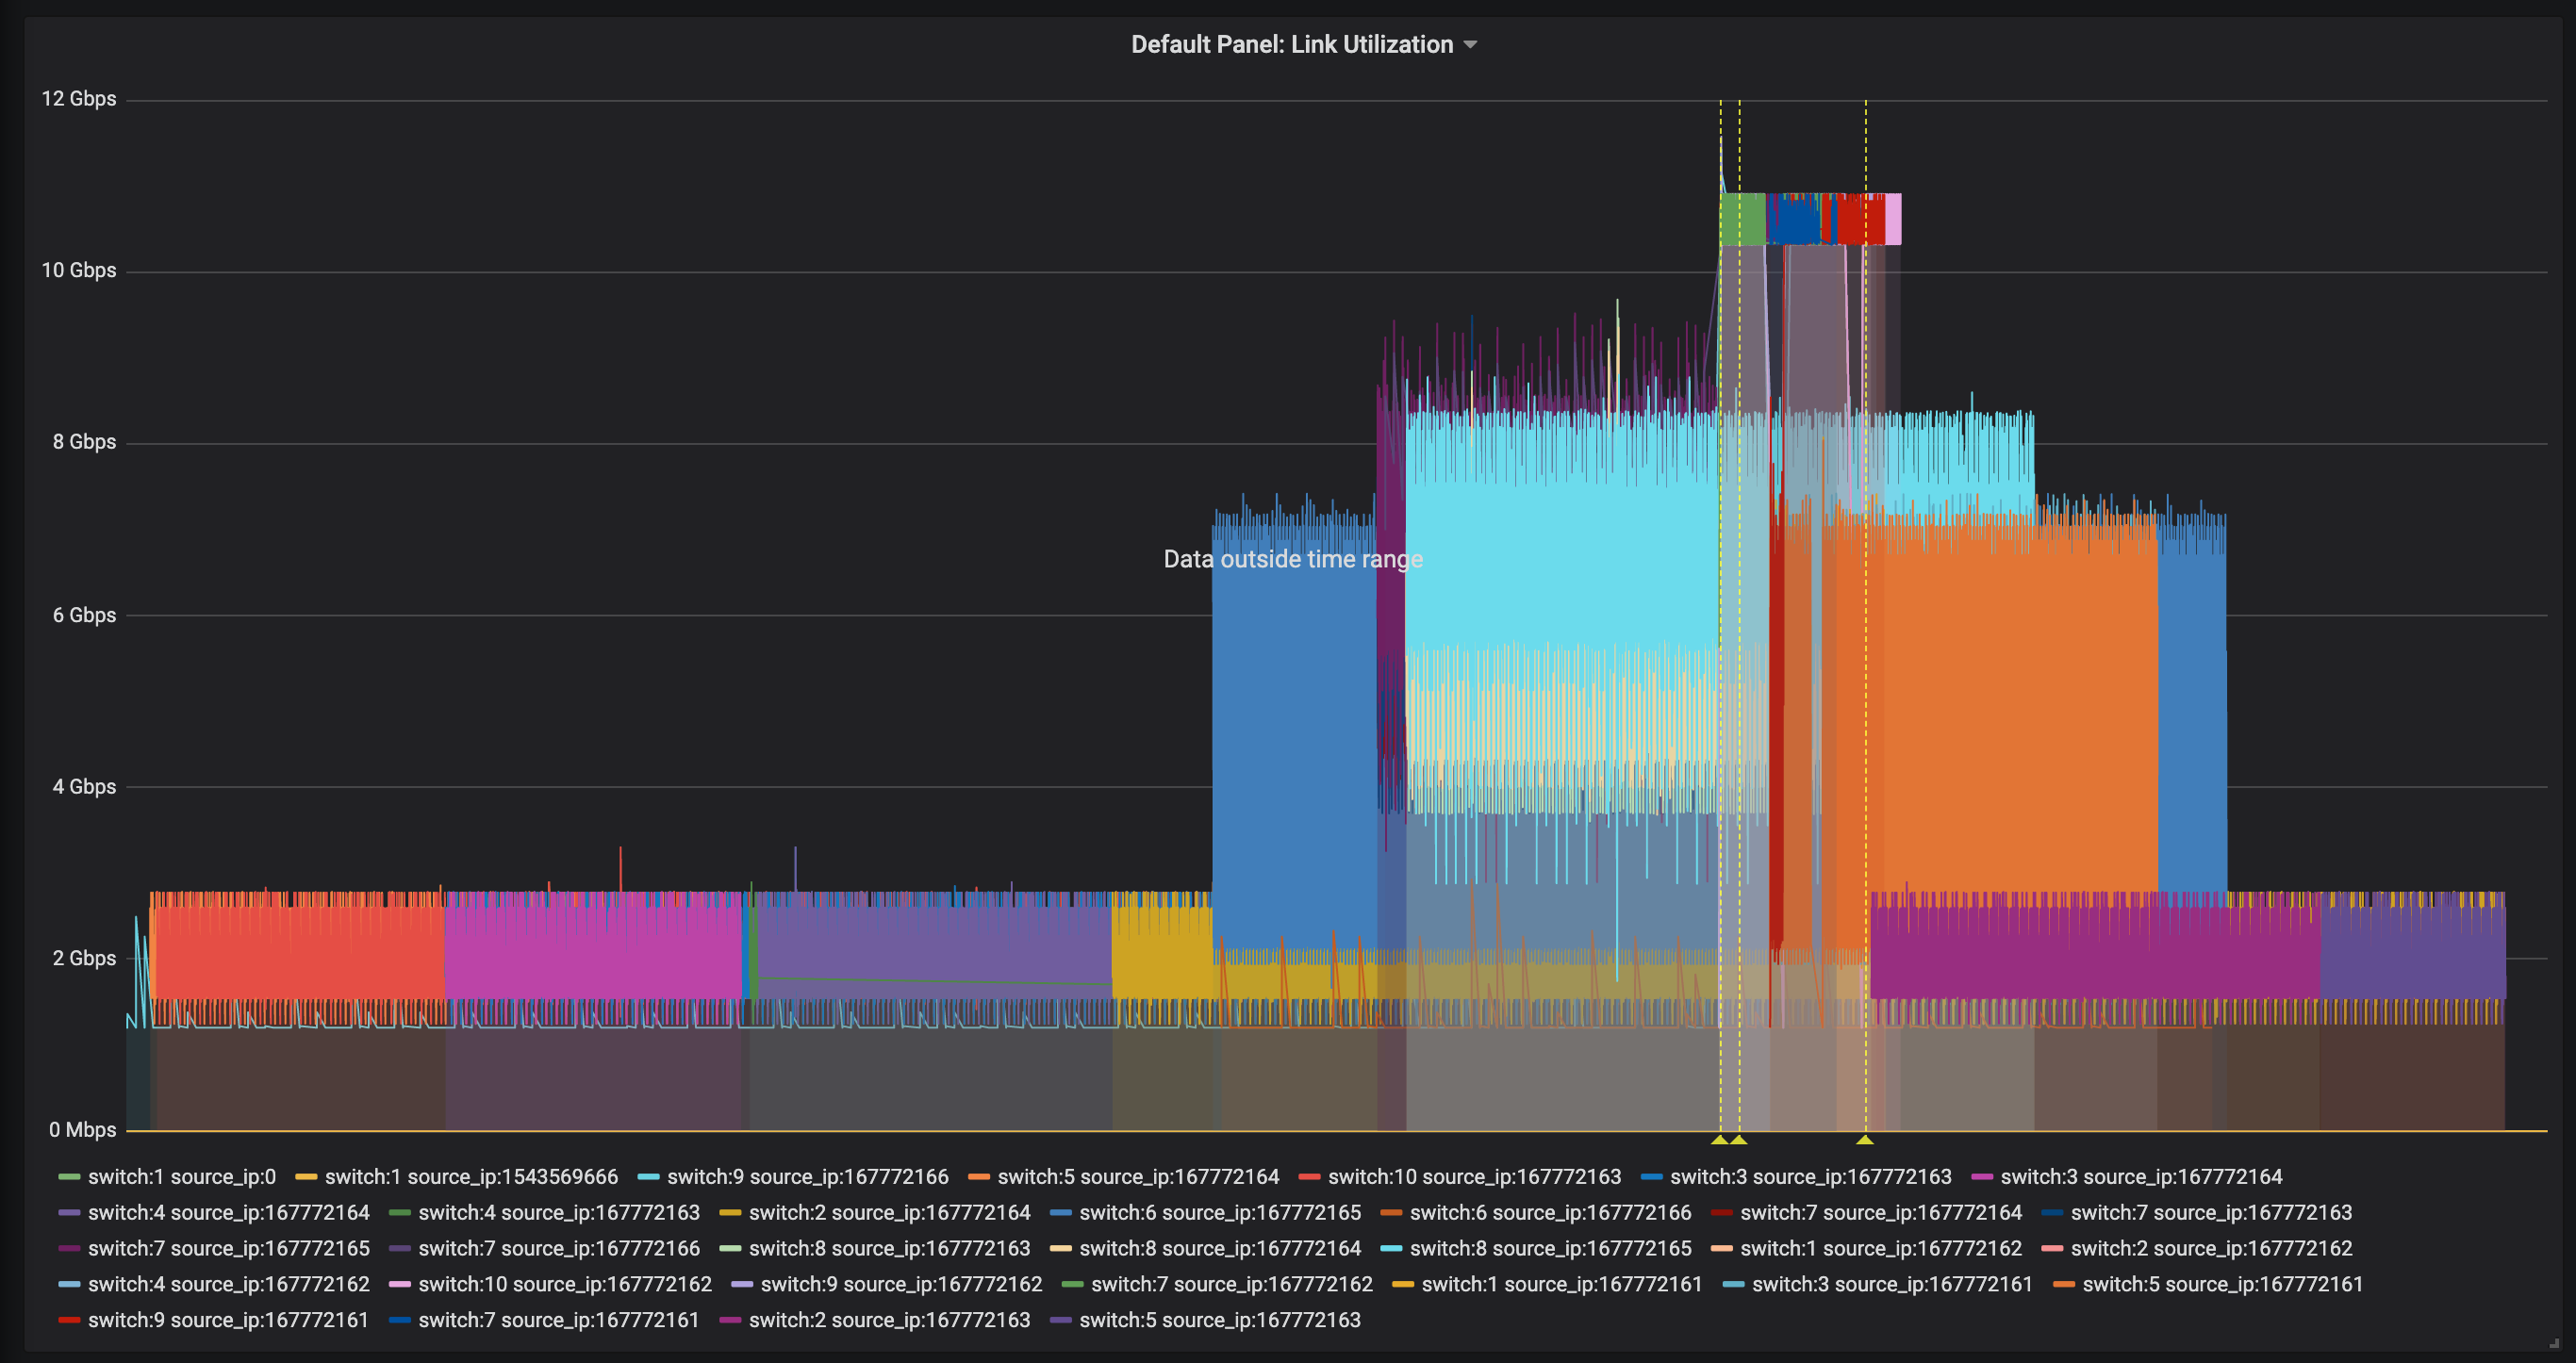
\includegraphics[width=1.0\columnwidth]{Figures/link_utilization_under.png}
		\rule{35em}{0.5pt}
	\caption[Link Utilization at Trigger Switch, Link Underprovisioning]{Link Utilization at Trigger Switch, Link Underprovisioning}
	\label{fig:link_utilization_under}
\end{figure}
\begin{figure}[htbp]
	\centering
		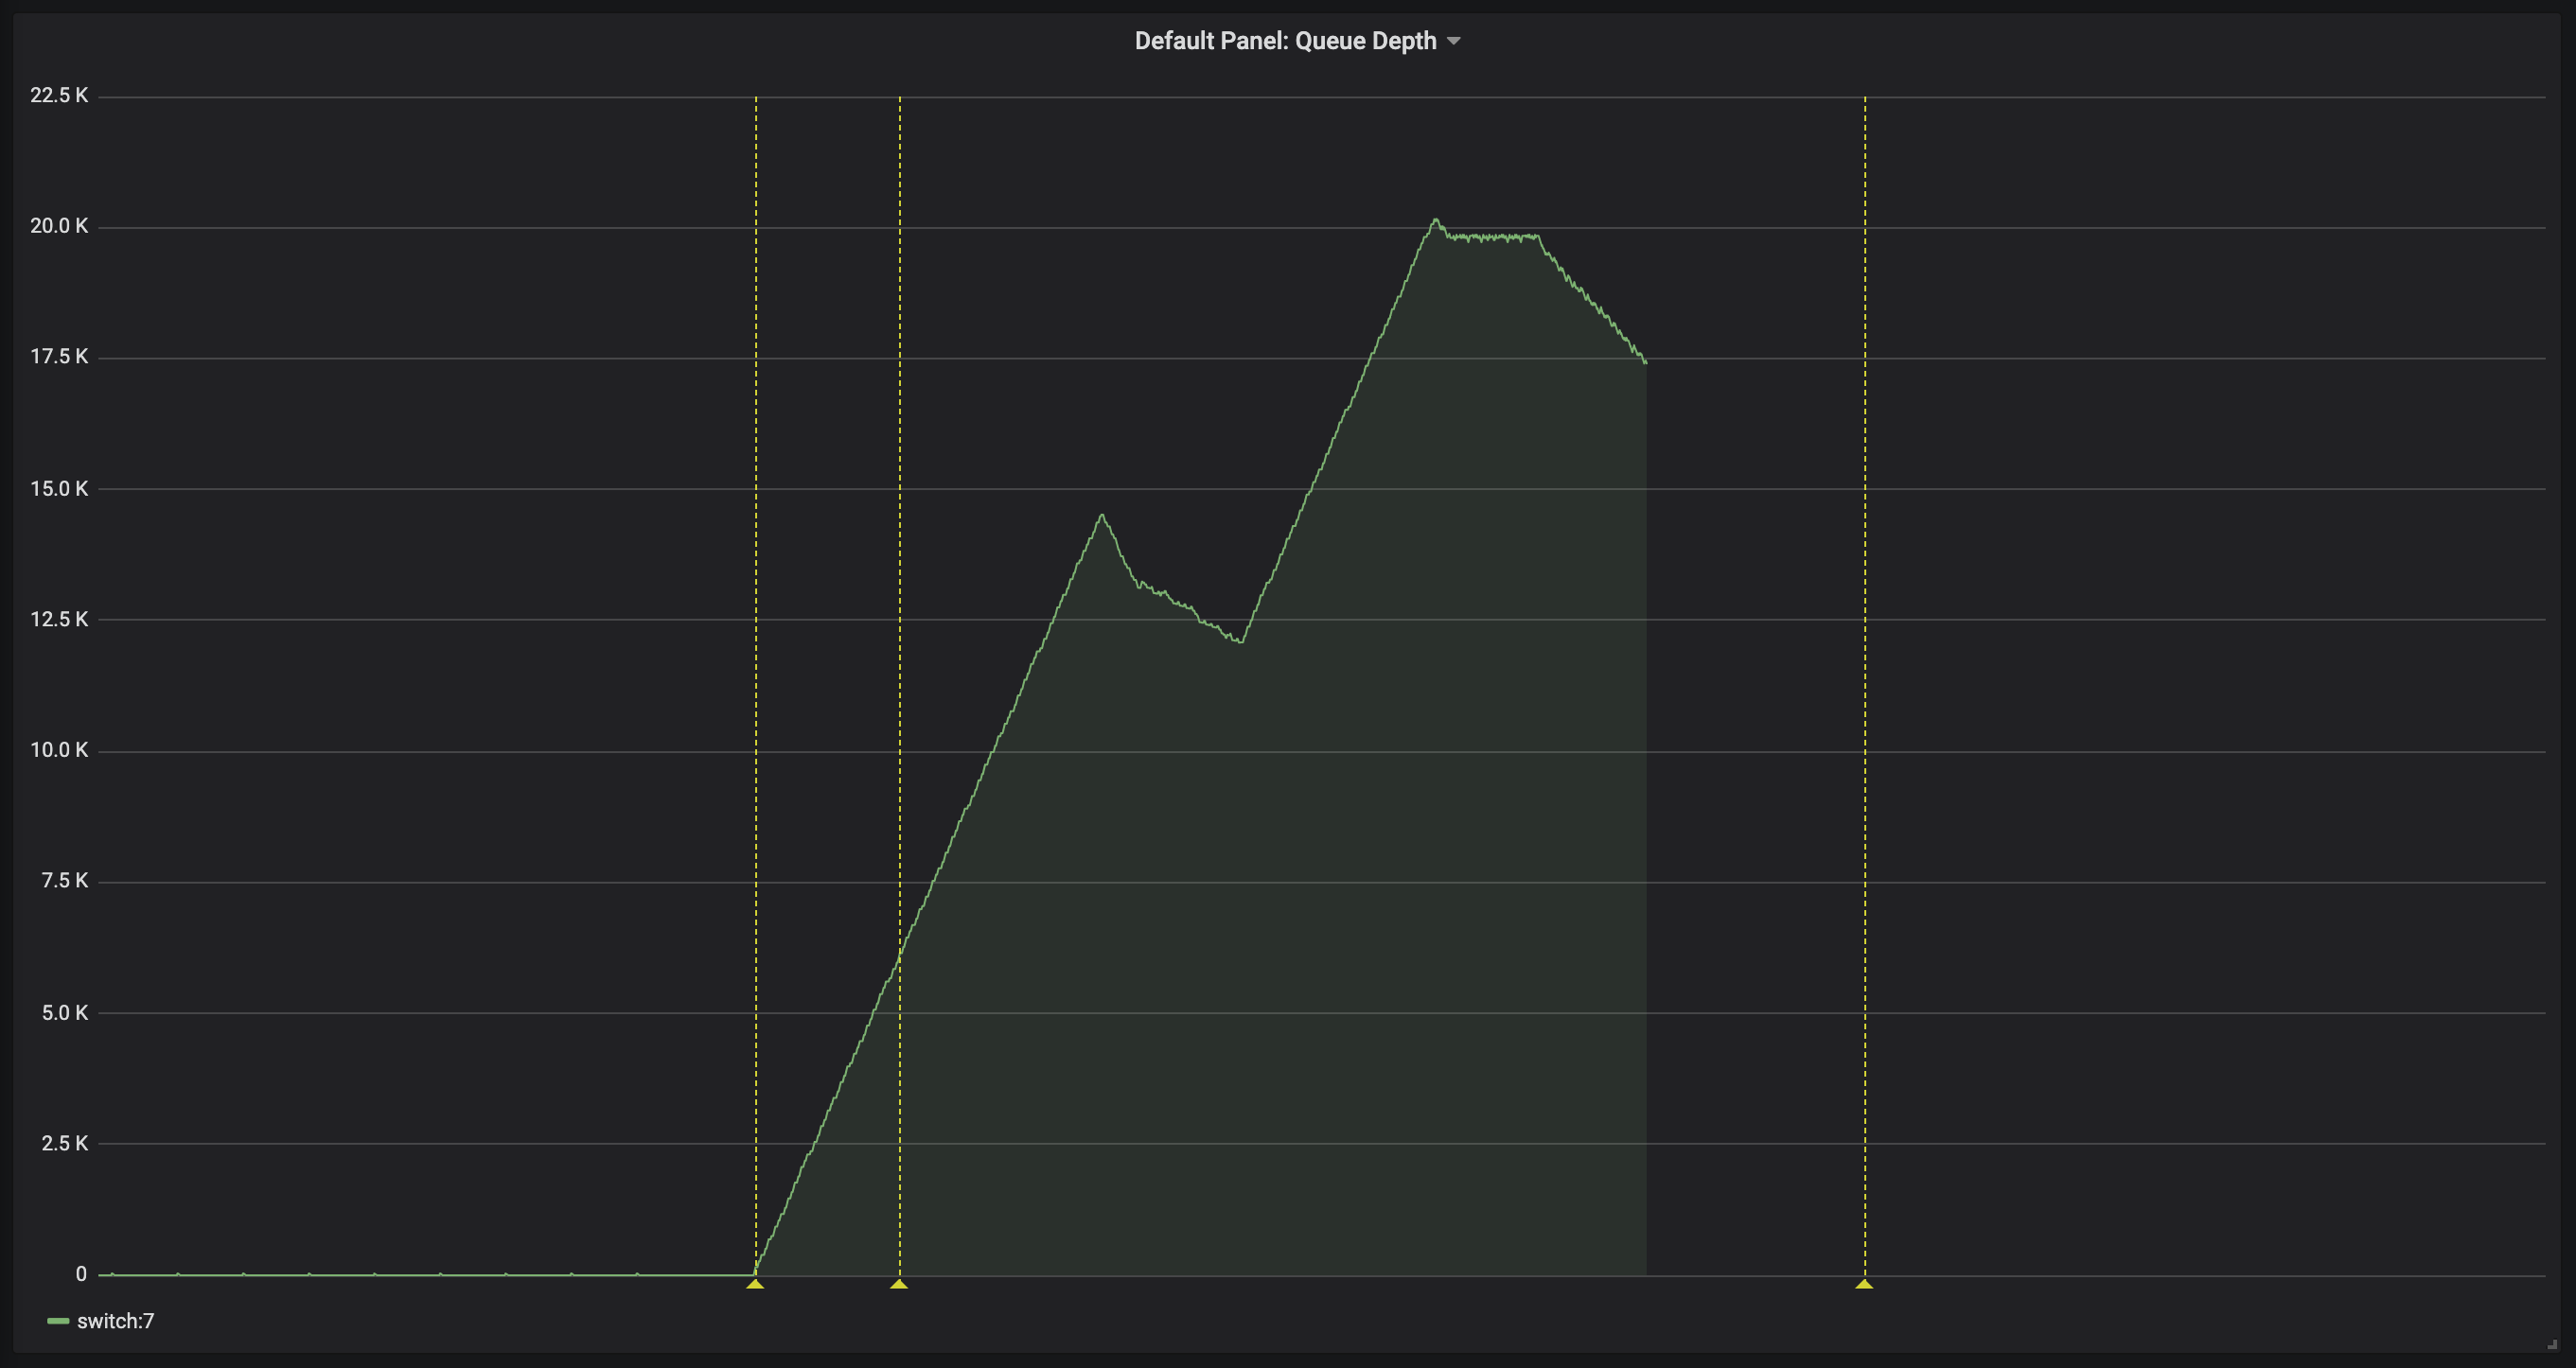
\includegraphics[width=1.0\columnwidth]{Figures/queue_depth_under.png}
		\rule{35em}{0.5pt}
	\caption[Queue Depth at Trigger Switch, Link Underprovisioning]{Queue Depth at Trigger Switch, Link Underprovisioning}
	\label{fig:queue_depth_under}
\end{figure}
\begin{figure}[htbp]
	\centering
		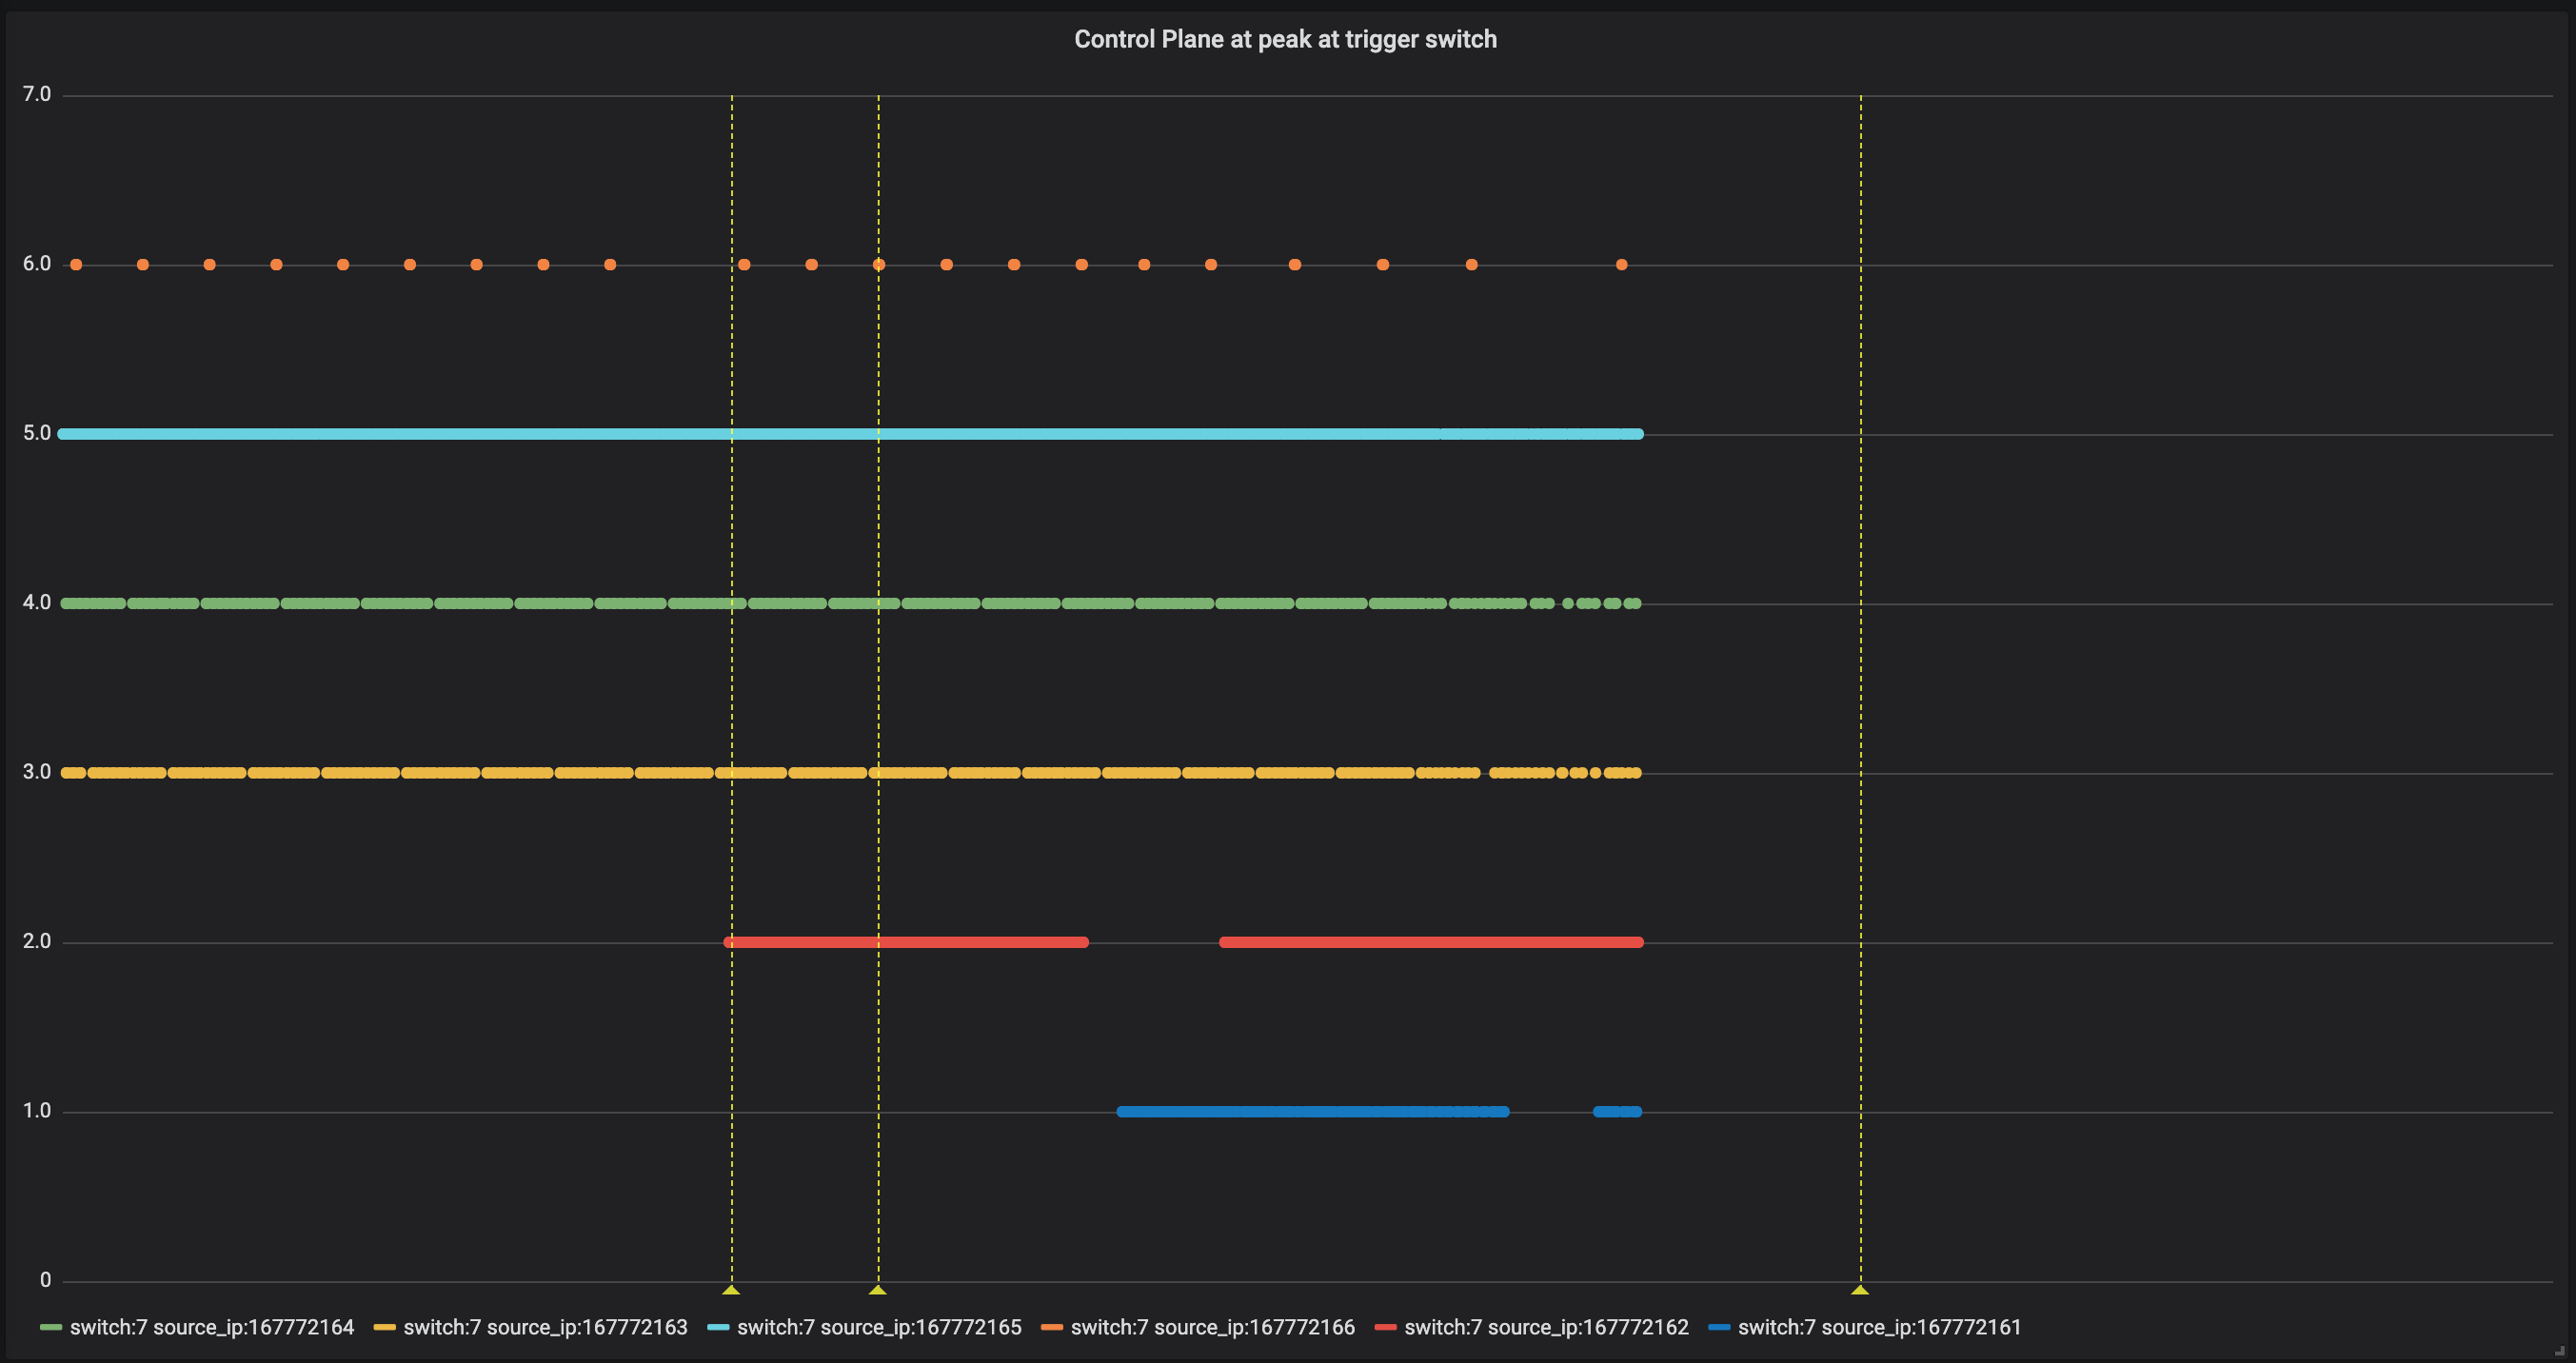
\includegraphics[width=1.0\columnwidth]{Figures/distribution_under.png}
		\rule{35em}{0.5pt}
	\caption[Packet Distribution at Trigger Switch, Link Underprovisioning]{Packet Distribution at Trigger Switch, Link Underprovisioning. Note the overlapping dots, showing link to be overutilized.}
	\label{fig:distribution_under}
\end{figure}
\section{Conclusions and further scope}

Based on the reasoning done in the preceding sections, a unified scheme to classify arbitrary scenarios based on the above discussion would be as follows:
\begin{itemize}
	\item Estimate the peak width in the graph
	\item If it is more than 1 millisecond, check if link is being overutilized. If so, it is probably a case of link underprovisioning.
	\item If it is less than 1 microsecond, calculate Jain's Fairness Index of packet distribution. If it is greater than 0.7, it is probably a synchronized incast. 
	\item Else, if it is less than 0.45, it is probably an asynchronous incast with heavy hitters present.
	\item Else (it is between 0.45 and 0.7), plot appropriate graphs for queue depth and link utilization and let the network operator deduce the exact problem.
\end{itemize}

As I further pursue my thesis, my goal is to isolate many such problems (two problems I currently have in mind are link failure 
and change of control plane policy), diagnose them on an individual basis, and at the end consolidate everything together into a single unified logic for diagnosing 
varied faults in a network.


%% Chapter Template

\chapter{Conclusion} % Main chapter title

\label{Chapter6} % Change X to a consecutive number; for referencing this chapter elsewhere, use \ref{ChapterX}

\lhead{Chapter 6. \emph{Conclusion}} % Change X to a consecutive number; this is for the header on each page - perhaps a shortened title

\section{Findings}
The goal of this thesis was to develop a monitoring system for data center networks using
data plane programmability and debate about the feasibility of a relational model for effectively querying the network. 
In chapter 4, we have 
demonstrated that with a relatively simple set of information about packets leaving switches, a number of quantities can be
derived which are hugely insightful. These quantities were then used in chapter 5 where we saw how a network
administrator could use the visualizations developed to gain an insight into the network. We established network visibility
through peak depth fairness calculations, plots of ingress throughputs and egress throughputs, and an ability to replay the
traffic through the network and see exactly how throughputs across links and queues in switches changed over time.
\section{Future Scope}
The natural next step in this direction is to investigate whether data plane programmability can be combined with
learning methods (techniques of deep learning and machine learning), to create autonomous, self driving networks which
can predict, based on incoming data, as to whether a fault is about to happen in the network and take remedial steps to prevent it.
In cases where the fault couldn't be predicted beforehand, the system can learn from new data and train itself to identify traffic
patterns better. Self driving autonomous data center networks can potentially save a lot of capital for technology companies through
better fault tolerance and fault recovery
as well as give them the ability to
provide better quality of service guarantees to customers.



%\input{Chapters/Chapter7}

%-------------------------------------------------------------------------------
%	THESIS CONTENT - APPENDICES
%-------------------------------------------------------------------------------

\addtocontents{toc}{\vspace{2em}} % Add a gap in the Contents, for aesthetics

\appendix % Cue to tell LaTeX that the following 'chapters' are Appendices

% Include the appendices of the thesis as separate files from the Appendices
% folder
% Uncomment the lines as you write the Appendices

% Appendix A

\chapter{Jain's Fairness Index} % Main appendix title

\label{AppendixA} % For referencing this appendix elsewhere, use \ref{AppendixA}

\lhead{\emph{Jain's Fairness Index}} % This is for the header on each page - perhaps a shortened title

A description of the Jain's Fairness Index

\begin{equation}
    \mathcal{J}\left(x_{1}, x_{2}, \ldots, x_{n}\right)=\frac{\left(\sum_{i=1}^{n} x_{i}\right)^{2}}{n \cdot \sum_{i=1}^{n} x_{i}^{2}}=\frac{\overline{\mathbf{x}}^{2}}{\overline{\mathbf{x}^{2}}}=\frac{1}{1+\widehat{c_{\mathrm{v}}^{2}}}
    \end{equation}

    Raj Jain's equation rates the fairness of a set of values where there are n users, each having an associated
    throughput value. This metric ranges from 1/n in the worst case to 1 in the best case.
    \newline
    In this thesis, the metric is normalized to a scale of 0 to 1 before comparing it to thresholds as mentioned in
    the thesis sections.
%% Appendix Template

\chapter{Grafana} % Main appendix title

\label{AppendixB} % Change X to a consecutive letter; for referencing this appendix elsewhere, use \ref{AppendixX}

\lhead{\emph{Grafana}} % Change X to a consecutive letter; this is for the header on each page - perhaps a shortened title

Grafana is a multi-platform open source analytics and interactive visualization software available since 2014. It provides charts, graphs, and alerts for the web when connected to supported data sources. It is expandable through a plug-in system. End users can create complex monitoring dashboards using interactive query builders.

As a visualization tool, Grafana is a popular component in monitoring stacks, often used in combination with time series databases such as Prometheus and Graphite; monitoring platforms such as Sensu, Icinga, Zabbix, Netdata, and PRTG; SIEMs such as Elasticsearch and Splunk; and other data sources.


%% Appendix Template

\chapter{The Debugger Application} % Main appendix title

\label{Appendix3} % Change X to a consecutive letter; for referencing this appendix elsewhere, use \ref{AppendixX}

\lhead{Appendix 3. \emph{The Debugger Application}} % Change X to a consecutive letter; this is for the header on each page - perhaps a shortened title

As part of the thesis, I have written a Debugger web application to visualize results
and navigate through a loaded trace. This appendix is meant to elaborate on the structure
of the web application. Further details and application code can be found on \url{https://github.com/sankalp-sangle/FlaskDebugger}

The home page of the application provides a recommendation on what could possibly be the cause of fault in the scenario.
\begin{figure}[htbp]
	\centering
		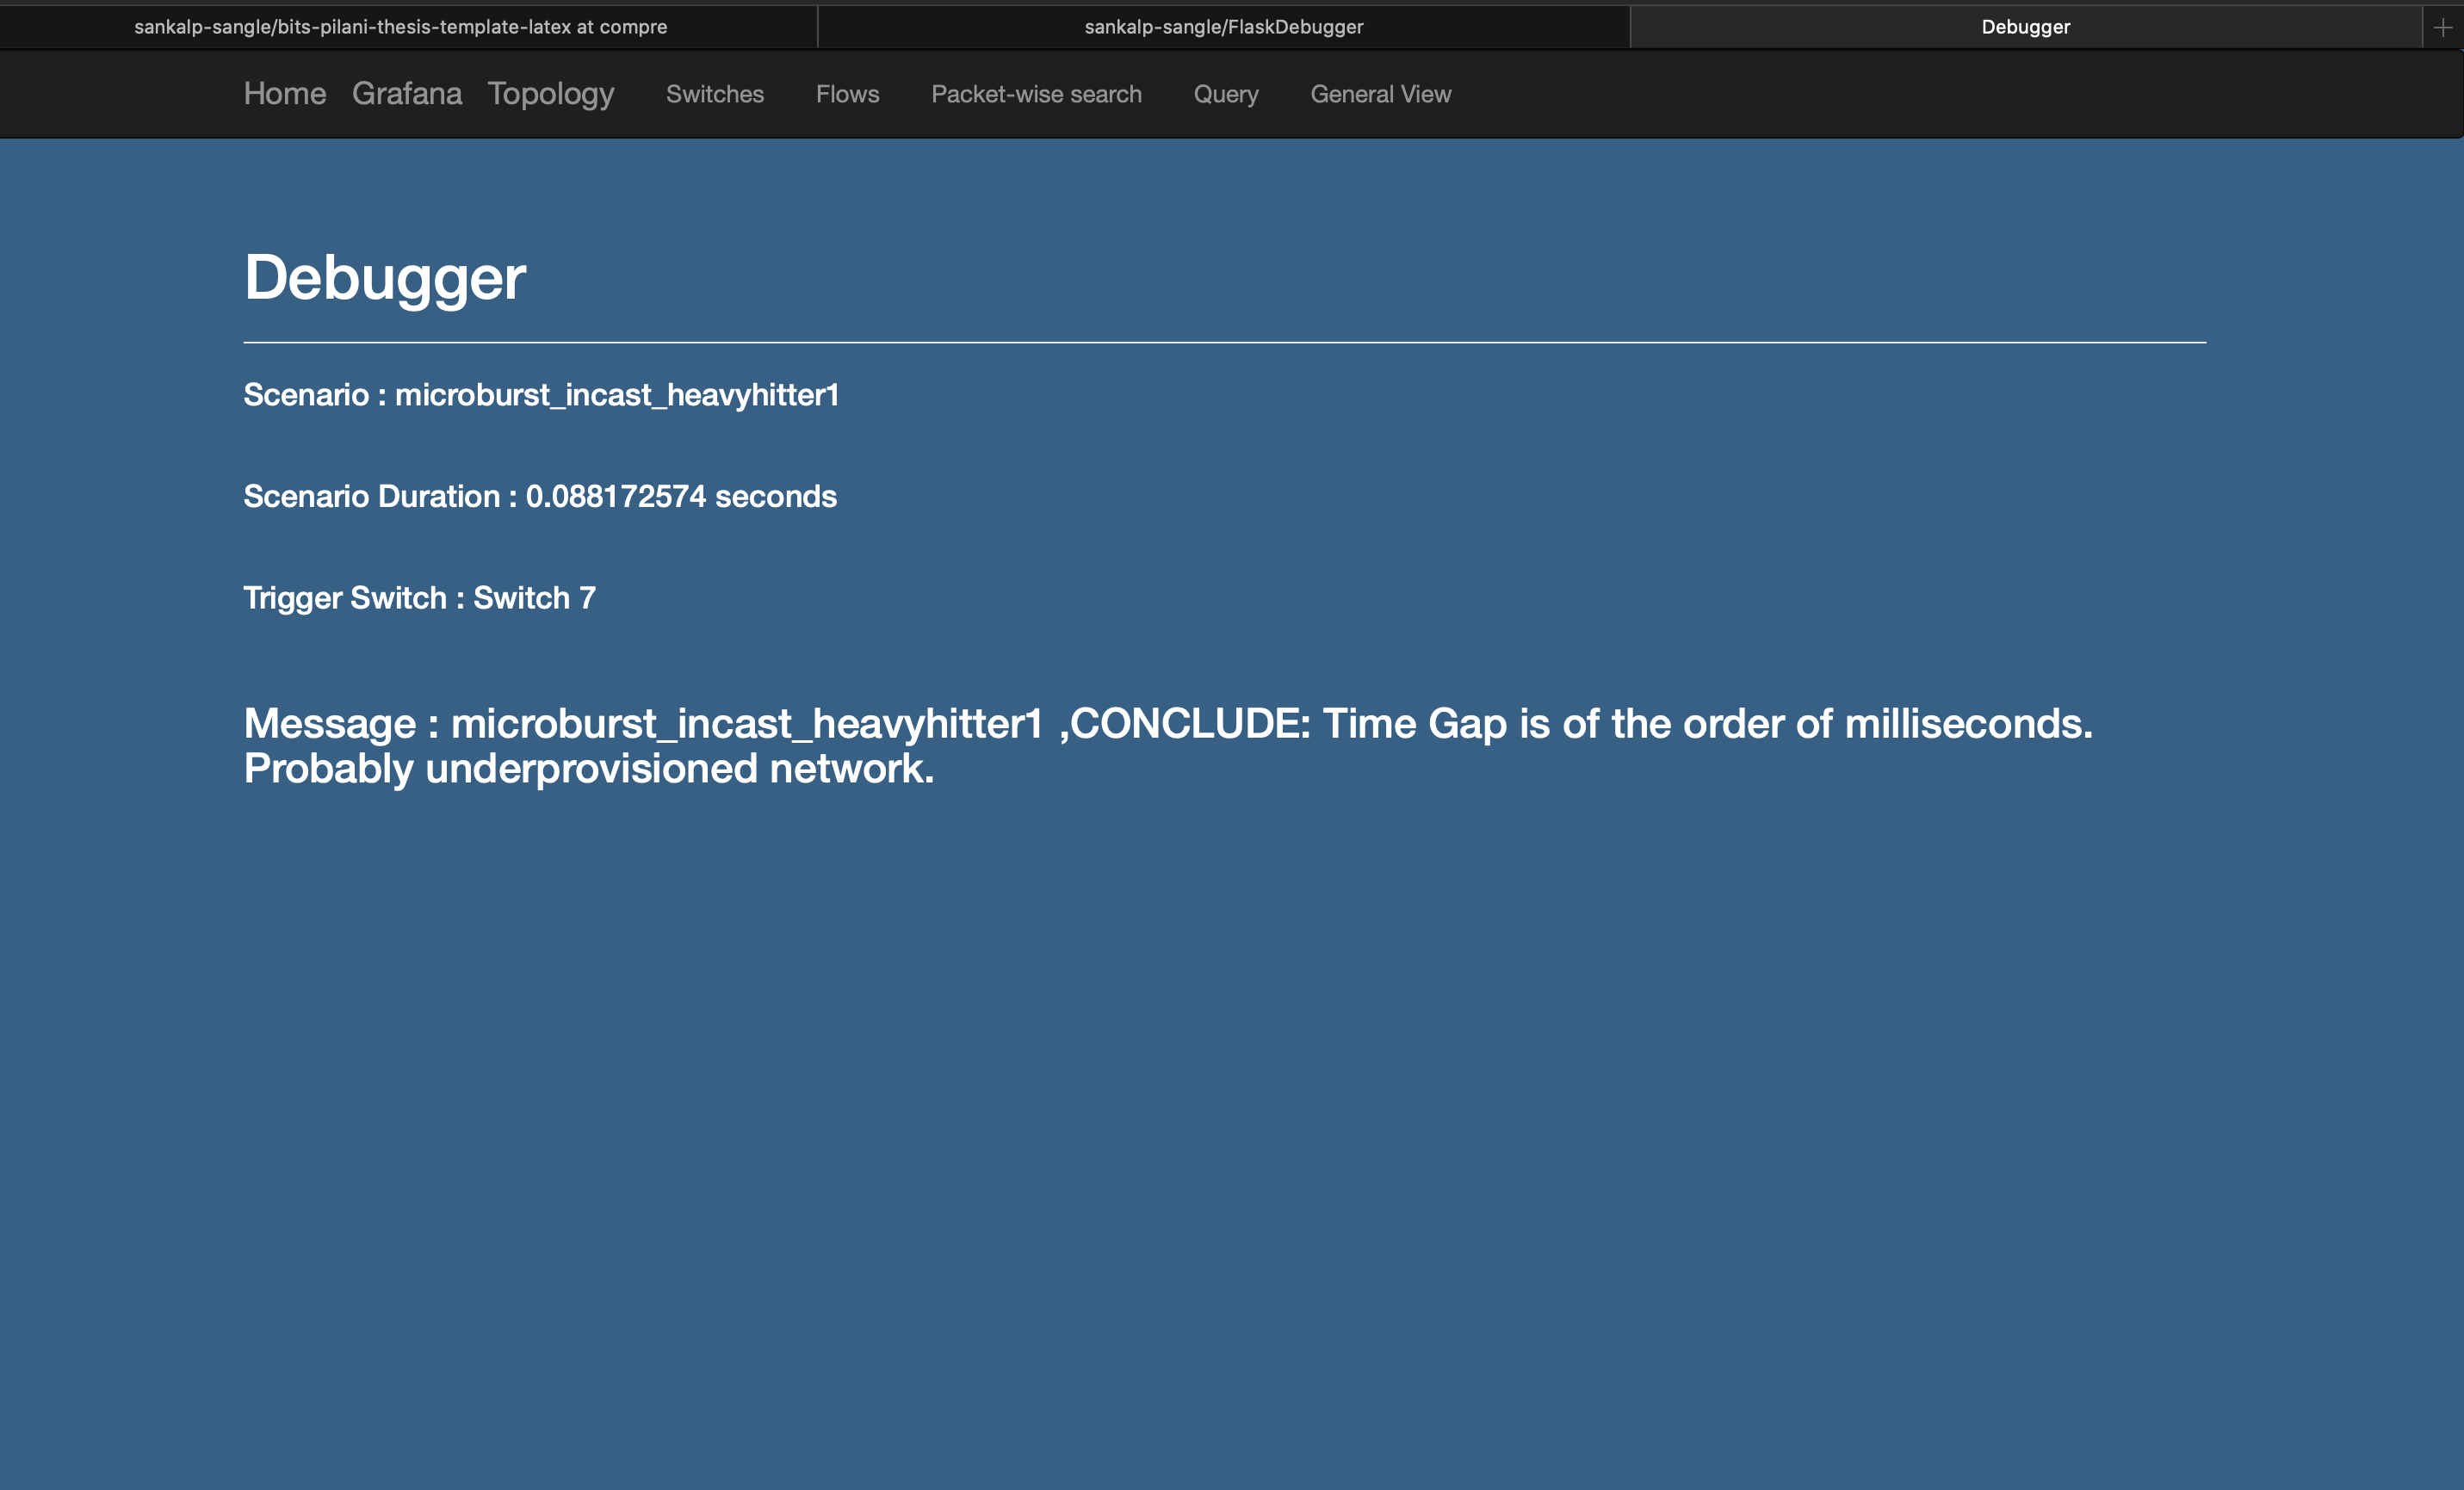
\includegraphics[width=1.0\columnwidth]{Figures/home.png}
		\rule{35em}{0.5pt}
	\caption[Home Page]{Home Page}
	\label{fig:home}
\end{figure}

From the home page, one can navigate to the topology page to view the network topology.
The switches are arranged in order of levels, with switches closer to the core being displayed at the top.
\begin{figure}[htbp]
	\centering
		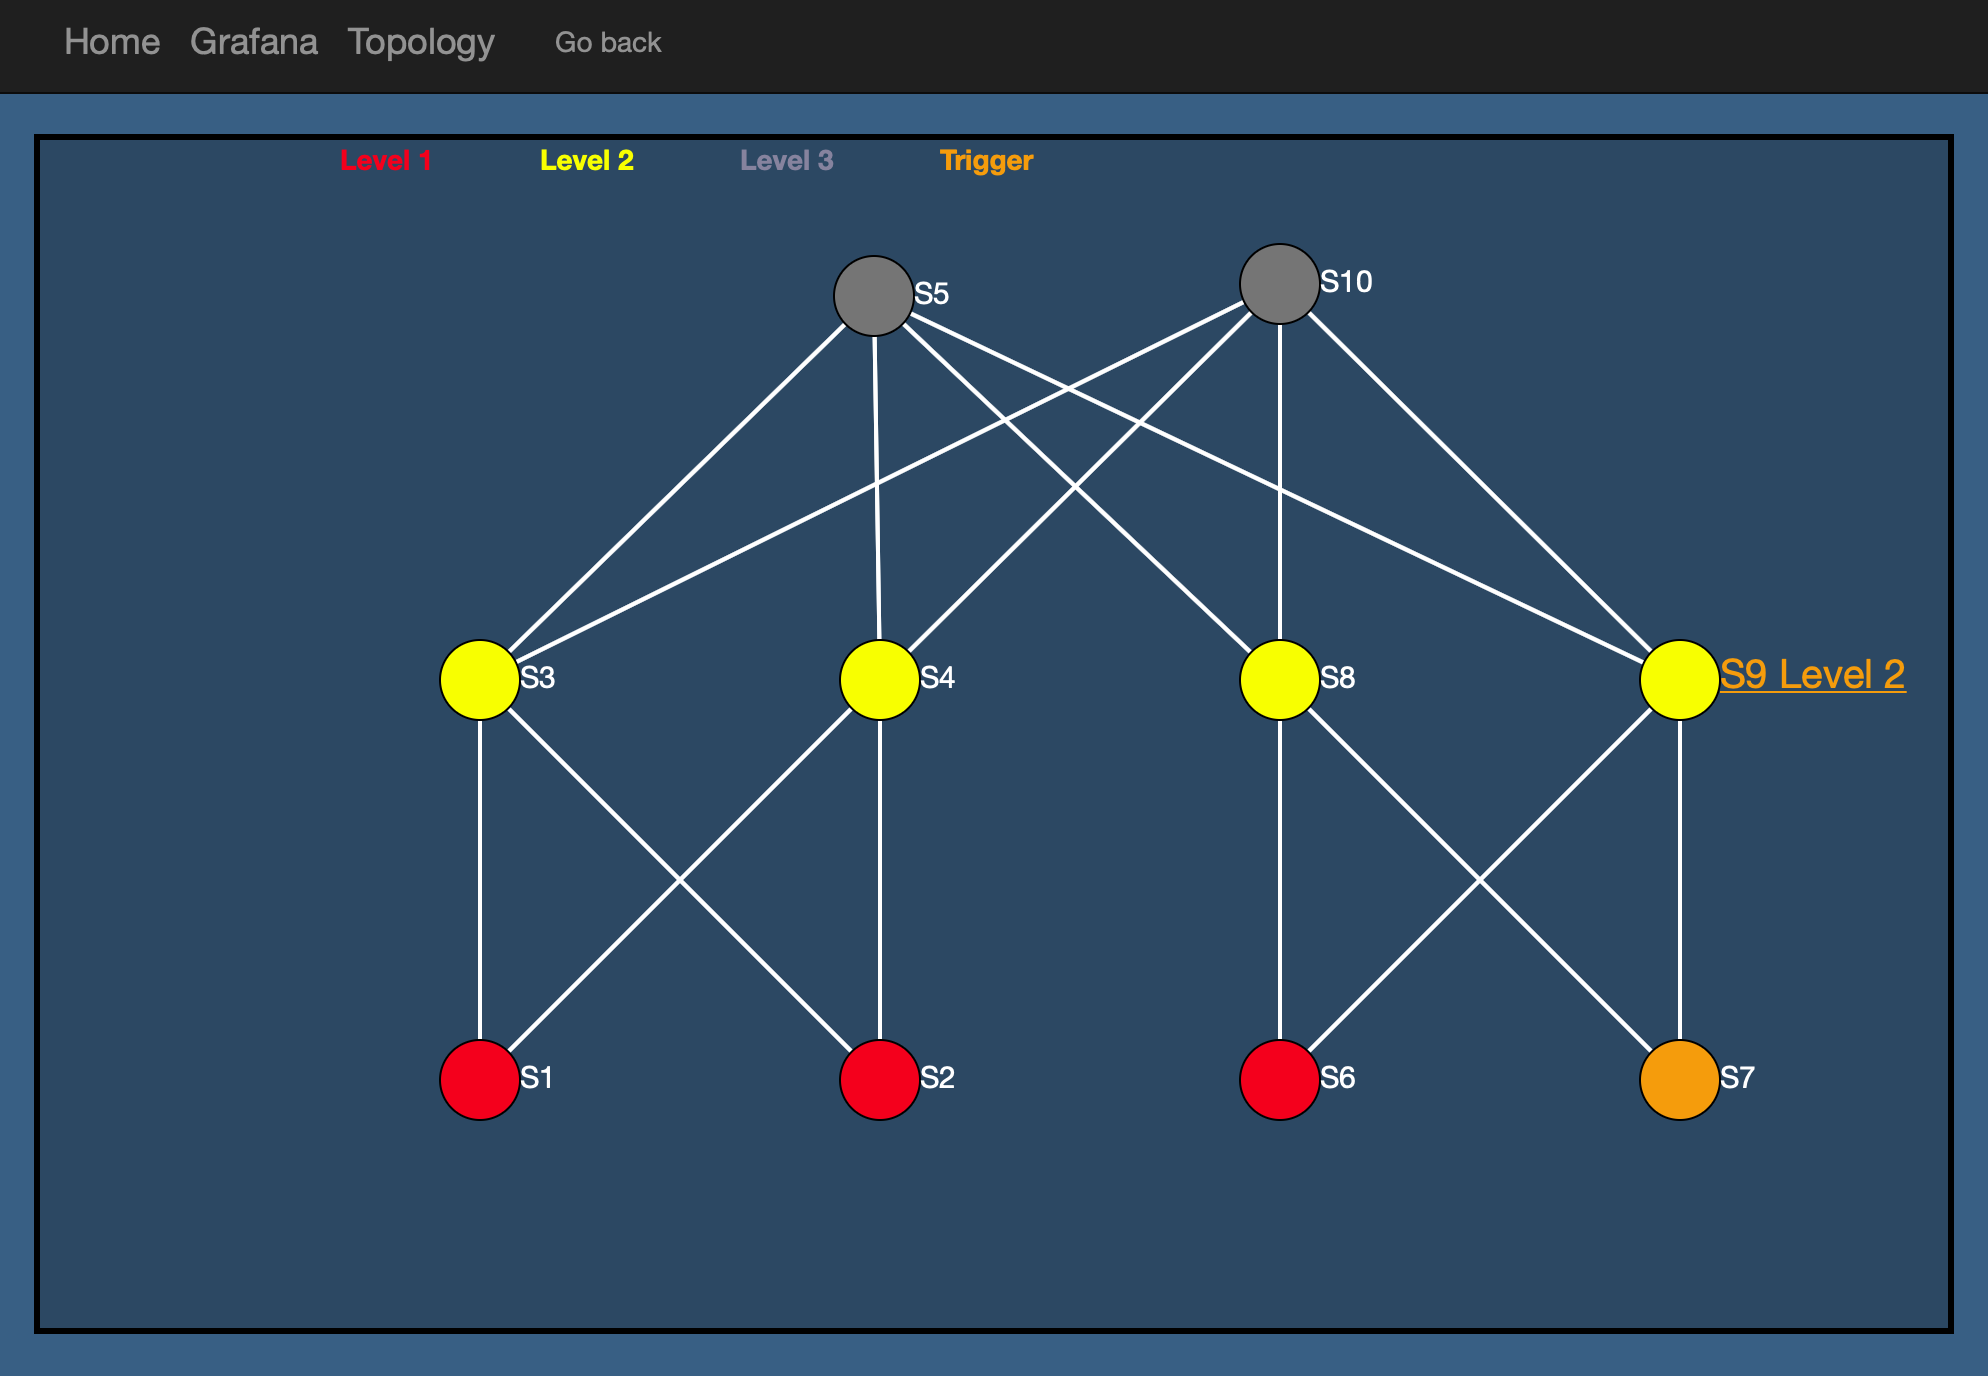
\includegraphics[width=0.85\columnwidth]{Figures/topo.png}
		\rule{35em}{0.5pt}
	\caption[Topology]{Topology}
	\label{fig:topo}
\end{figure}

One can click on any of the switches to see details about that switch.
\begin{figure}[htbp]
	\centering
		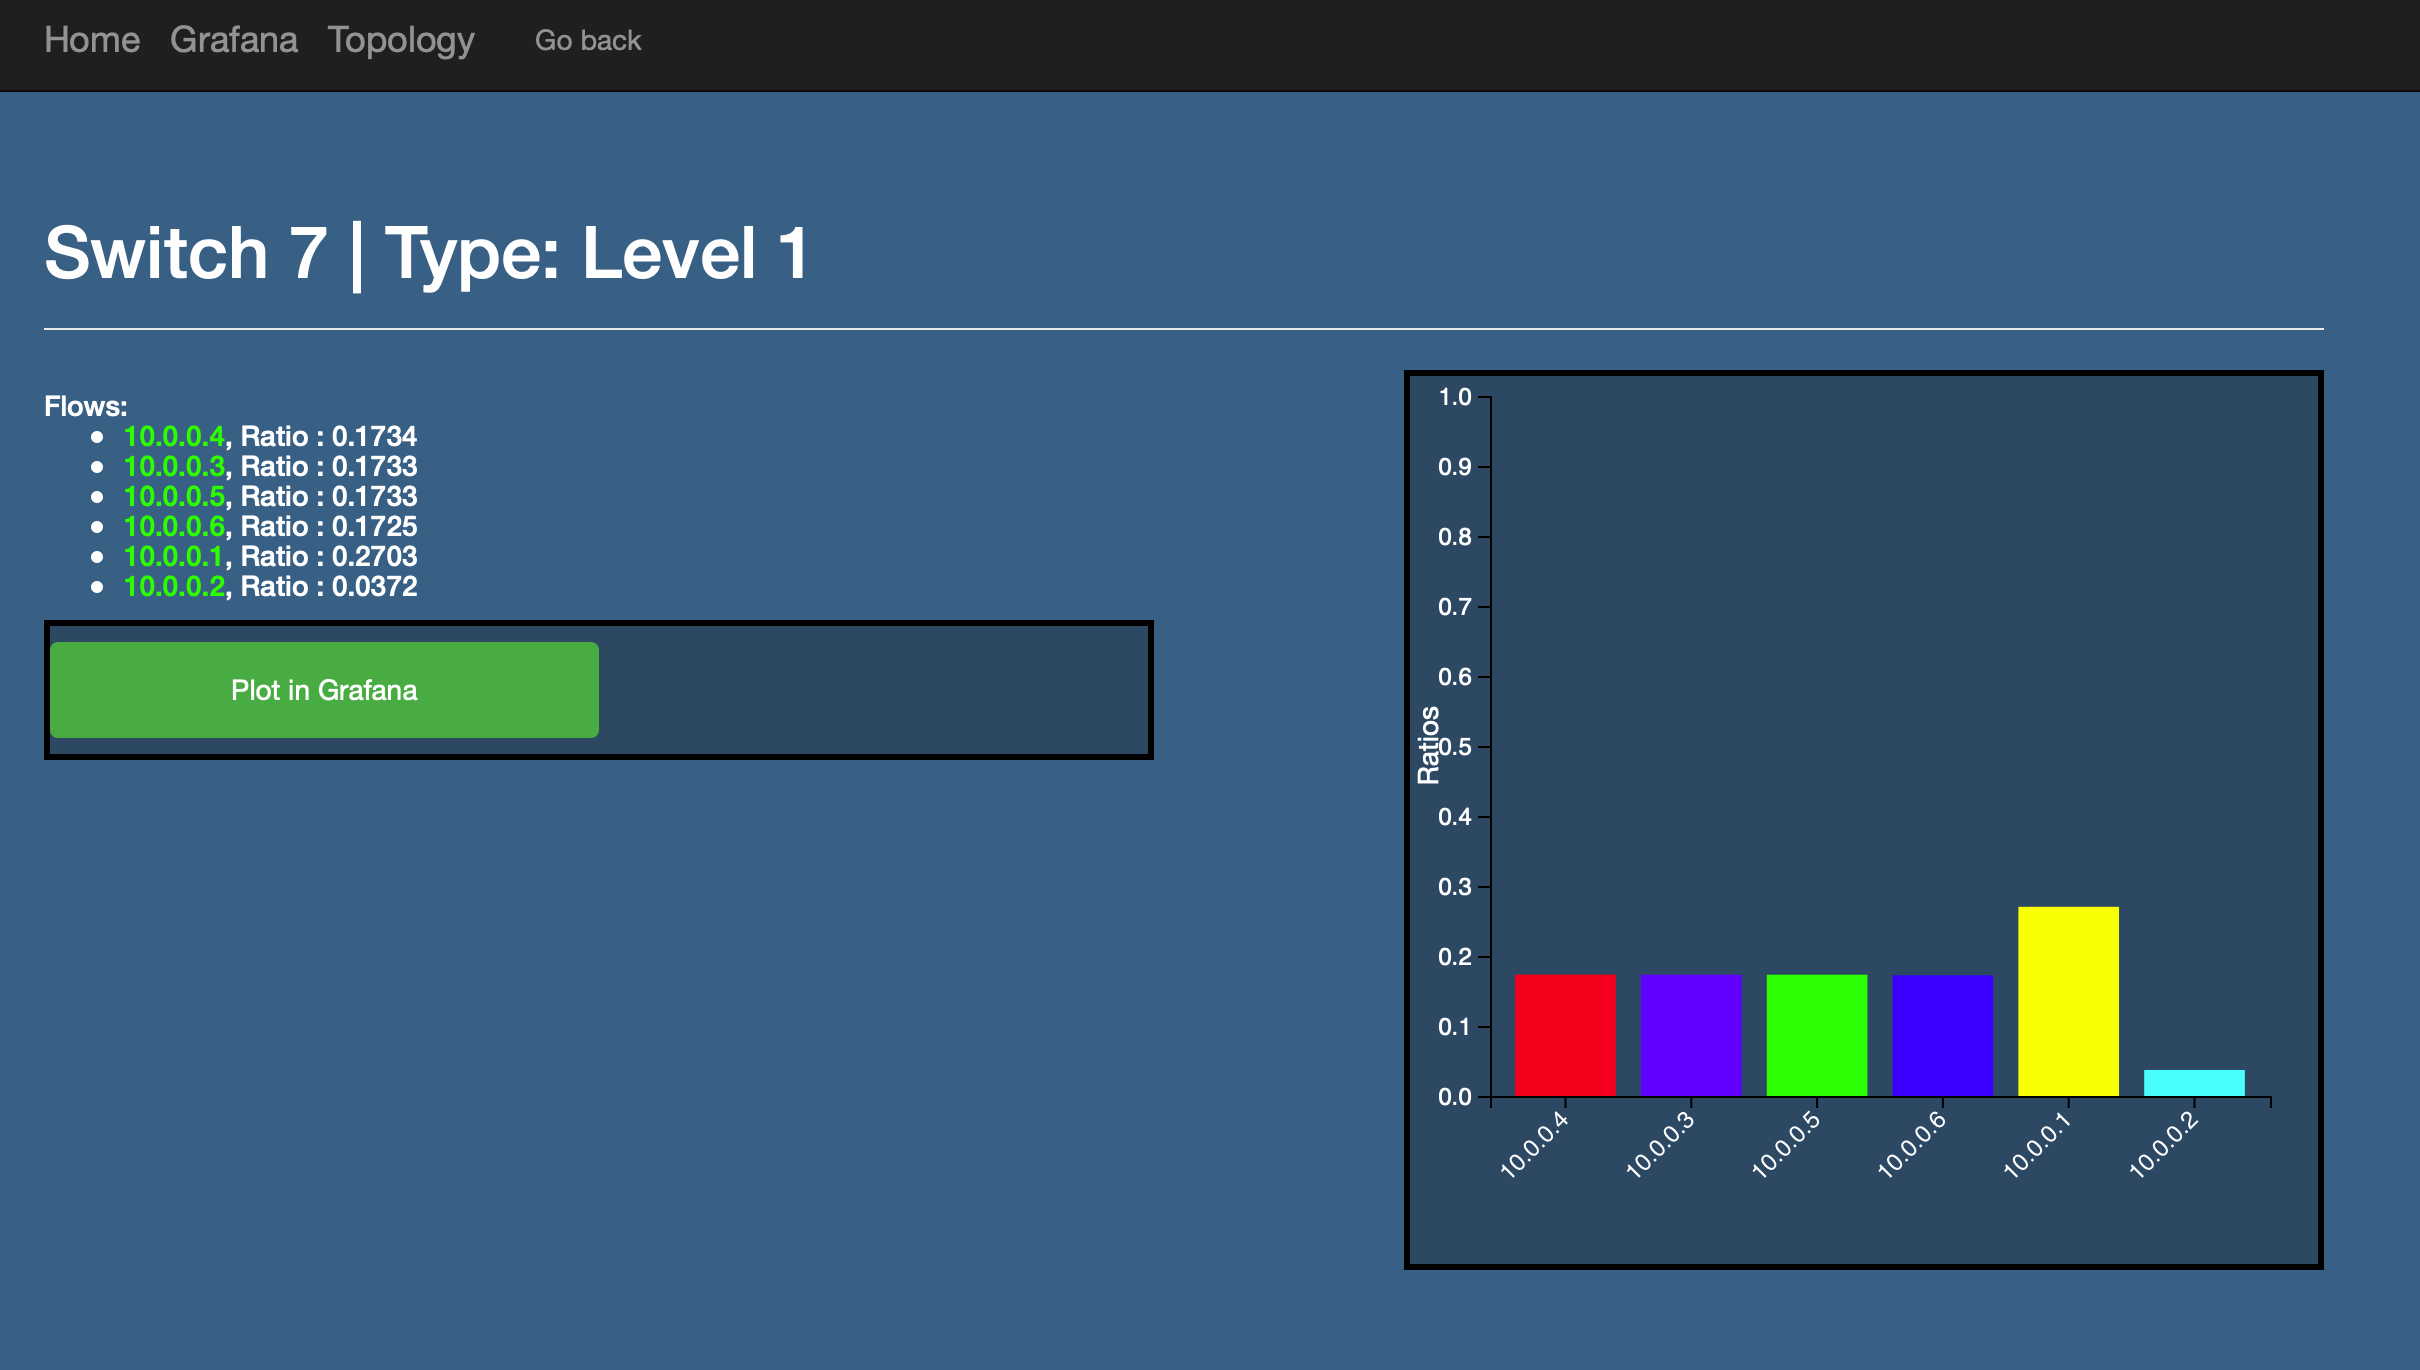
\includegraphics[width=0.85\columnwidth]{Figures/switch.png}
		\rule{35em}{0.5pt}
	\caption[Switch Information]{Information about switch 7}
	\label{fig:switch}
\end{figure}

\newpage

If one wishes to view details about a particular flow, one can click on the
the IP address to view more information such as switches visited.

\begin{figure}[htbp]
	\centering
		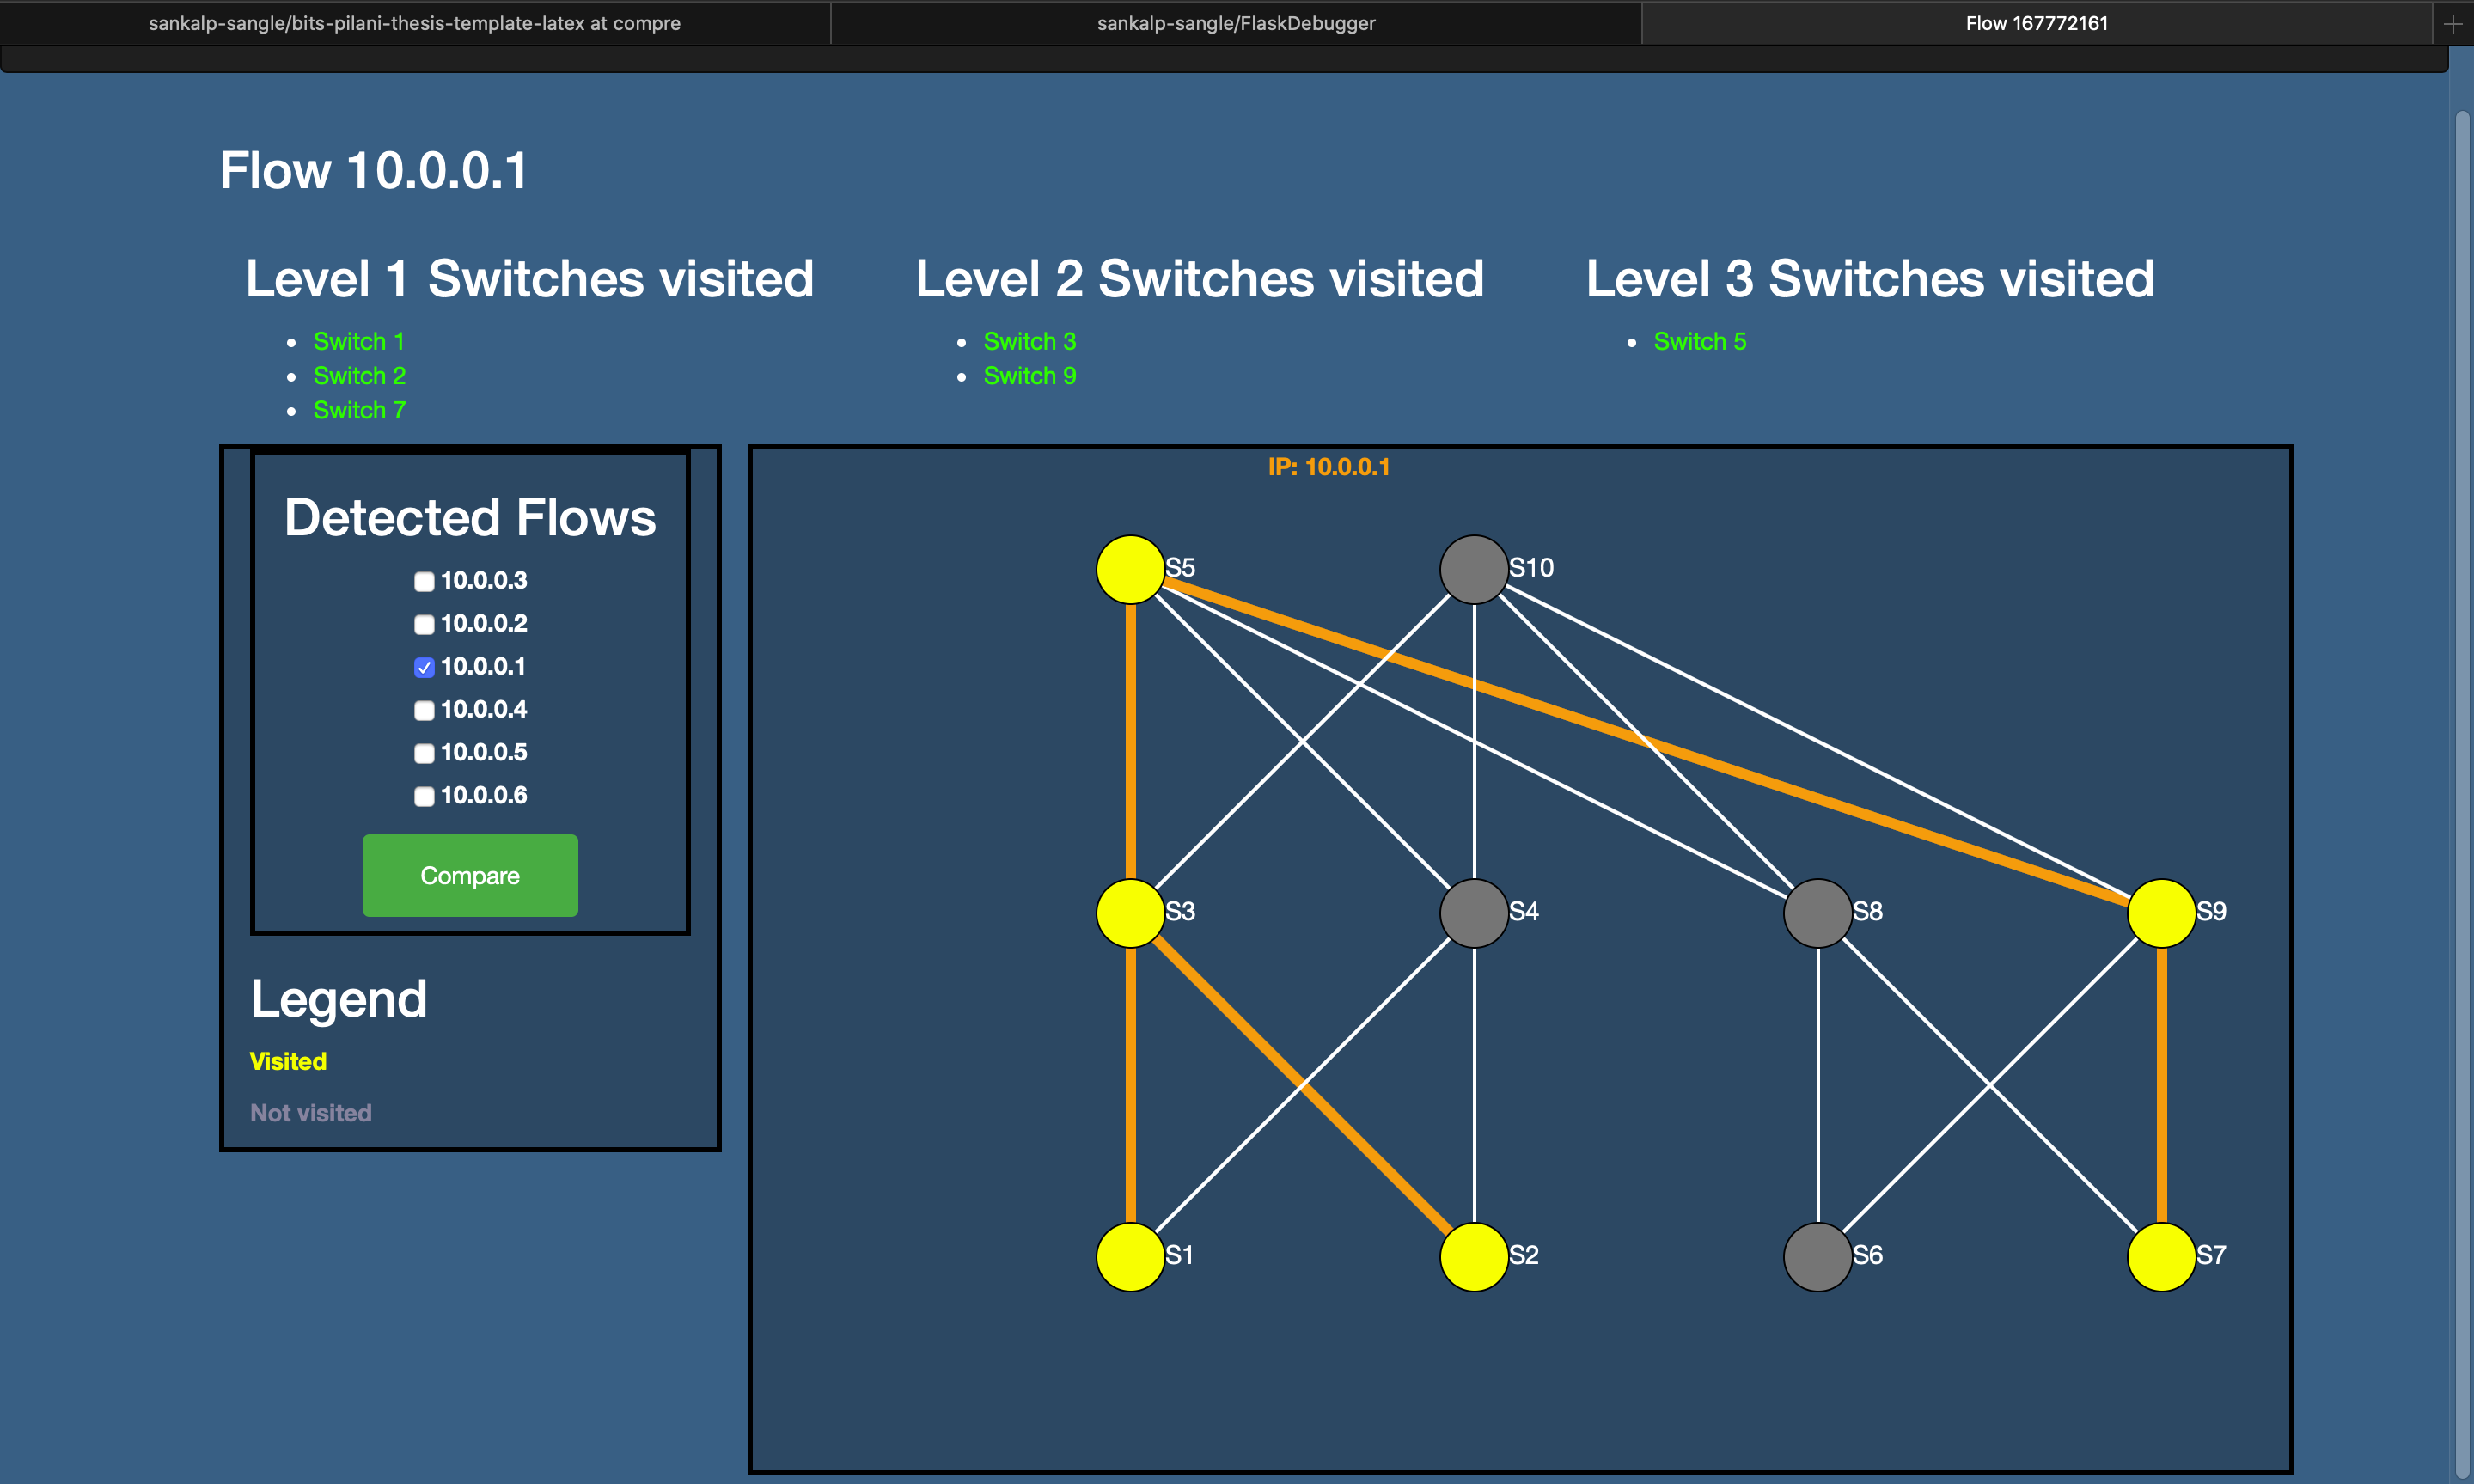
\includegraphics[width=1.0\columnwidth]{Figures/flow.png}
		\rule{35em}{0.5pt}
	\caption[Flow Information]{Flow Information}
	\label{fig:flow}
\end{figure}

Finally, if one wishes to see a birds eye view of the topology and replay it back, one can
do so via the General View tab. We have options to pause, play, speed up and slow down the playback.

\begin{figure}[htbp]
	\centering
		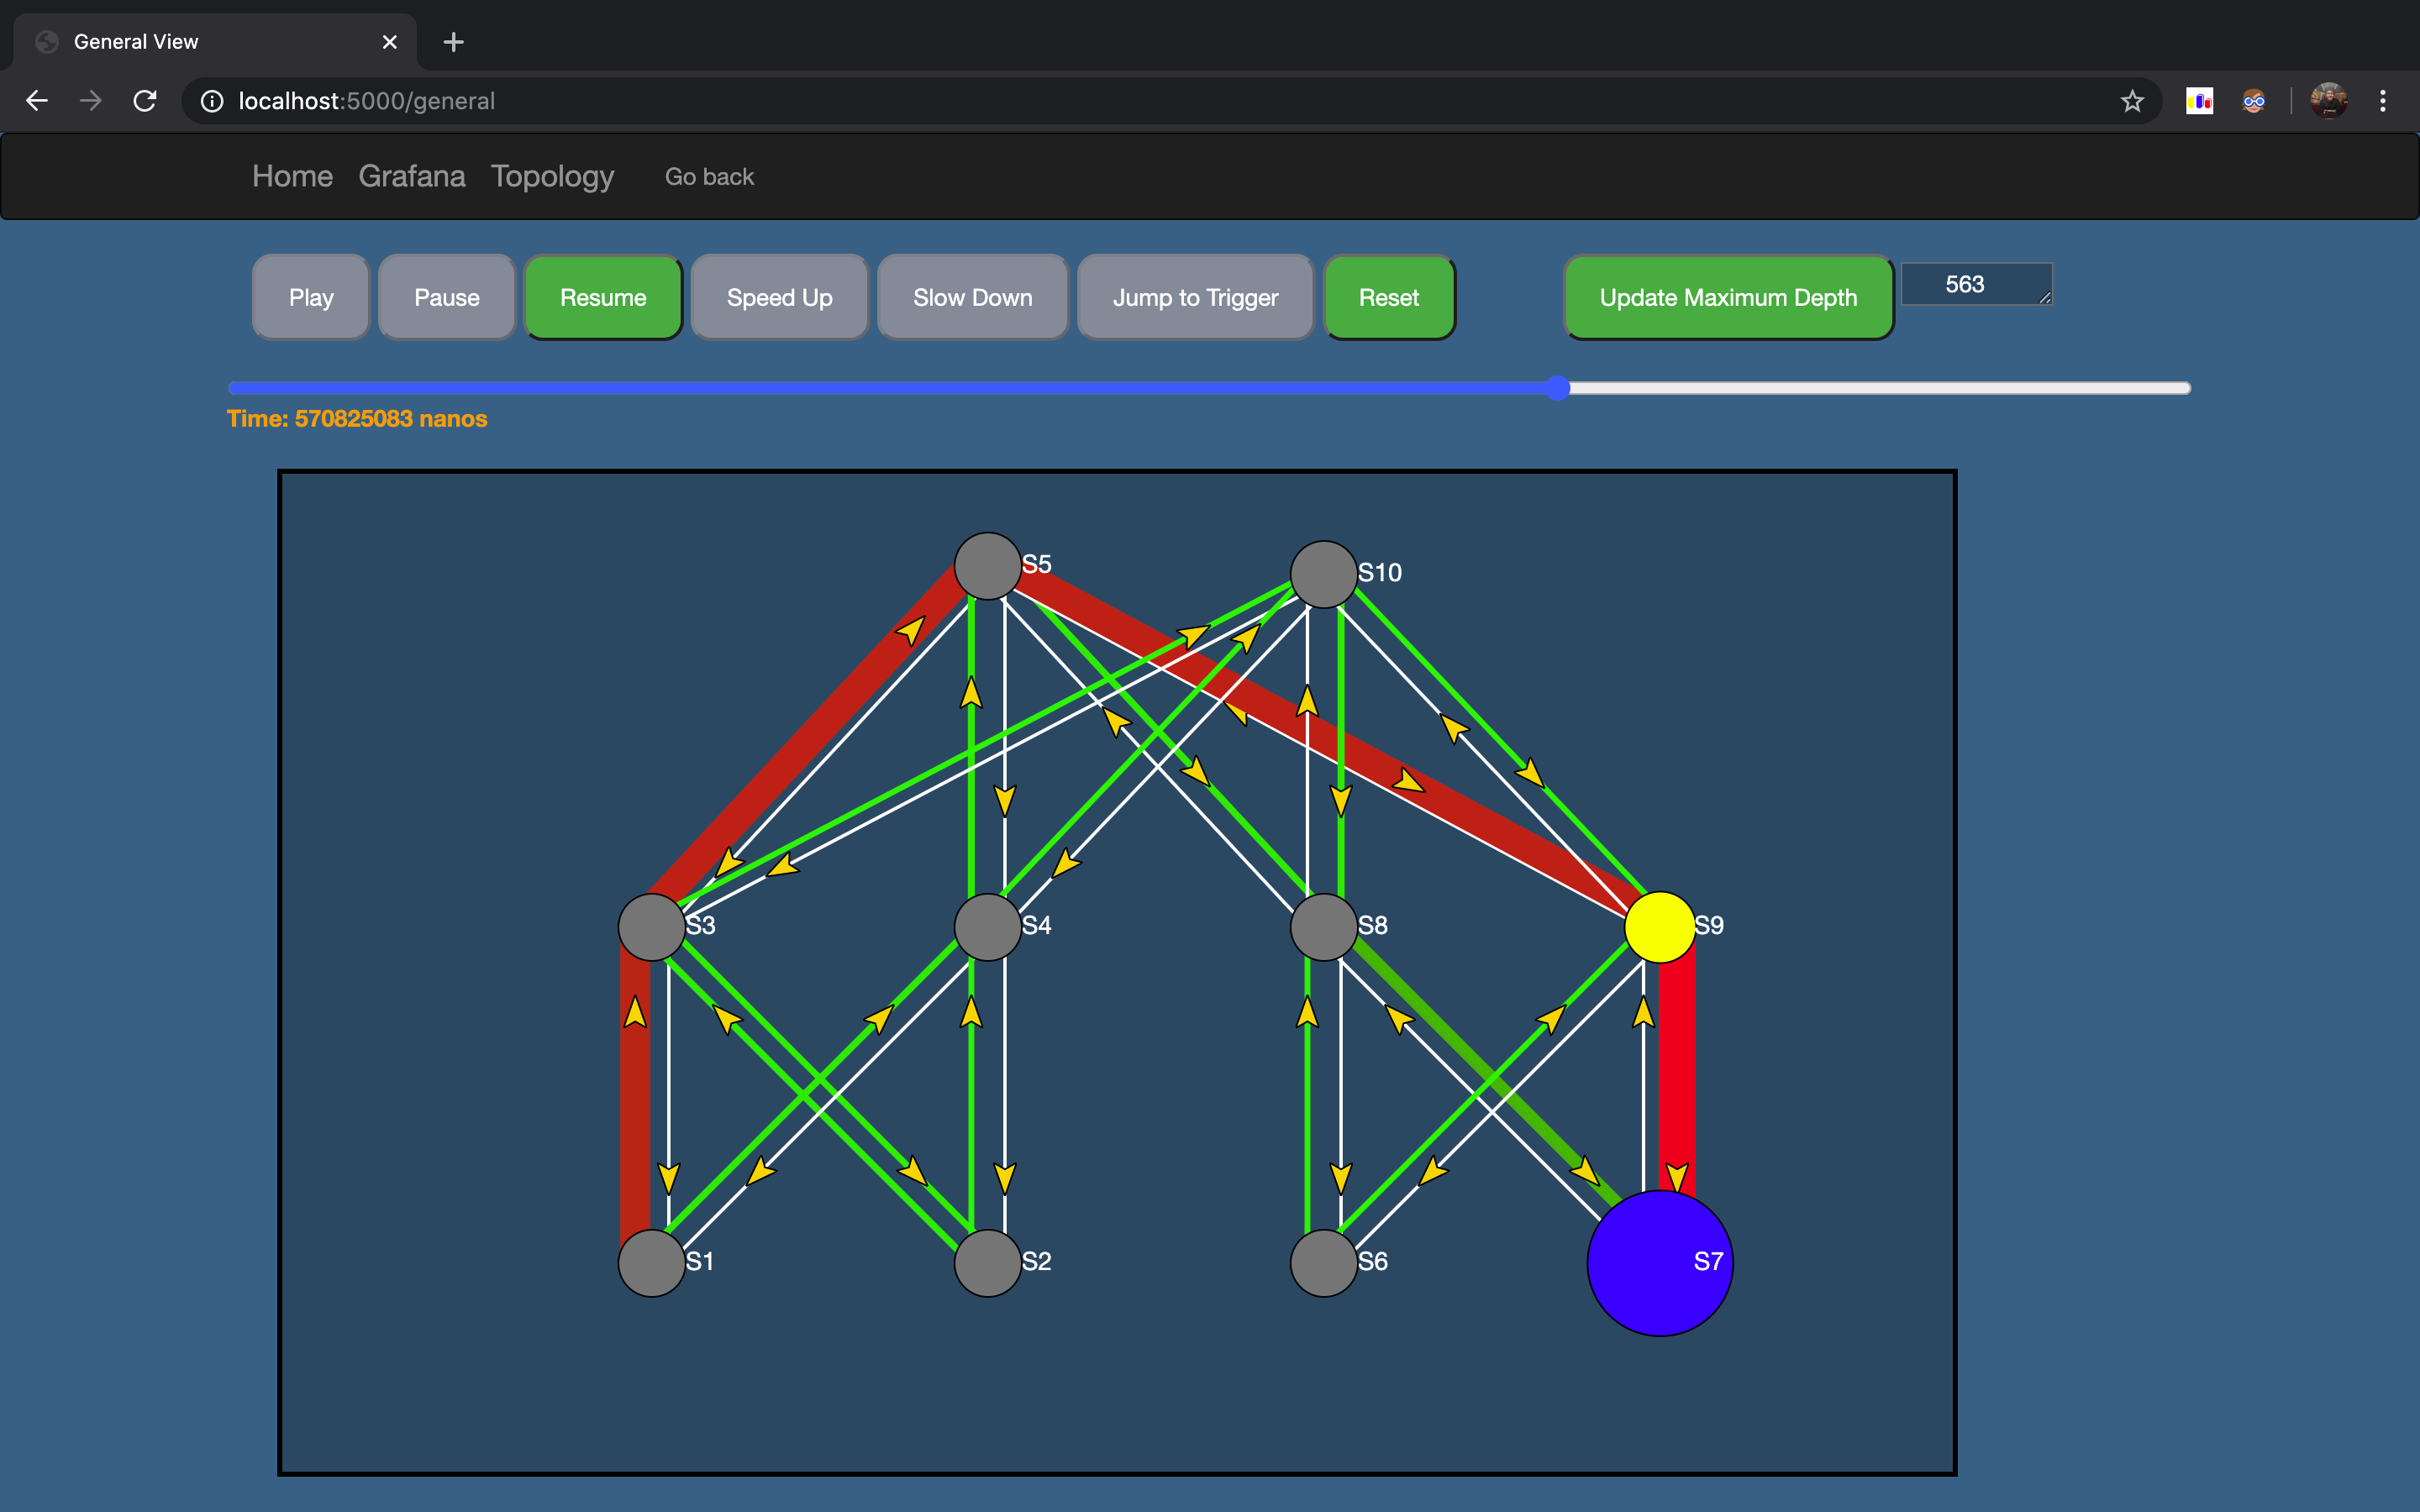
\includegraphics[width=1.0\columnwidth]{Figures/genview.png}
		\rule{35em}{0.5pt}
	\caption[Birds eye view]{A birds eye view of the scenario}
	\label{fig:birdseye}
\end{figure}

\addtocontents{toc}{\vspace{2em}} % Add a gap in the Contents, for aesthetics

\backmatter

%-------------------------------------------------------------------------------
%	BIBLIOGRAPHY
%-------------------------------------------------------------------------------

\label{Bibliography}

\lhead{\emph{Bibliography}} % Change the page header to say "Bibliography"

\printbibliography

\end{document}
